% !TeX spellcheck = en_GB
% encoding: utf8
% !TEX encoding = utf8
% !TEX program = pdflatex
% !BIB program = biber

\documentclass[11pt,oneside,a4paper]{article}

\usepackage[cmex10]{amsmath}
\usepackage[utf8]{inputenc}
\usepackage[T1]{fontenc}
\usepackage[colorlinks]{hyperref}
\usepackage[left=2.5cm, right=2.5cm, top=2.5cm, bottom=2.5cm]{geometry}
\usepackage{bm}
%\usepackage{plotstable}
\usepackage{graphicx}
\usepackage{float}
\usepackage{subcaption}
\usepackage[linesnumbered,ruled,vlined,onelanguage]{algorithm2e}
\usepackage{algorithmic}
\usepackage{mathtools}
%\usepackage[]{algorithmic}
\usepackage{array}

\usepackage{array}
\usepackage{makecell}
\usepackage{csvsimple}
\usepackage{booktabs}
\usepackage{xargs}
\usepackage{color, colortbl}
\usepackage{footmisc}

\usepackage{ifthen}




%%%%%
%%  Comments 
%%%%%
\usepackage{xargs}



\newcommand{\Fig}[1]{Fig.~\ref{#1}}

\usepackage{fourier} 
\usepackage{array}
\usepackage{makecell}
\usepackage{csvsimple}
\usepackage{booktabs}

\renewcommand\theadalign{bc}
\renewcommand\theadfont{\bfseries}
\renewcommand\theadgape{\Gape[4pt]}
\renewcommand\cellgape{\Gape[4pt]}
\renewcommand{\labelenumii}{\theenumii}
\renewcommand{\theenumii}{\theenumi.\arabic{enumii}.}
\usepackage{tabularx}
%\usepackage{soul}
\usepackage{xargs}

\newcommand{\twc}[1]{\textcolor{red}{\textbf{TW}: #1}}
\usepackage{hyperref} %<--- Load after everything else

%%%%%
%%   Definicja wymagań
%%%%


\usepackage[backend=biber,maxnames=10,style=numeric,sorting=nty,abbreviate=false,giveninits=true,language=english]{biblatex}
\addbibresource{../meros.bib}


\newcommand{\req}[1]{\textbf{\texttt{R#1}}}
\newcommand\mycommfont[1]{\footnotesize\ttfamily\textcolor{blue}{//#1\\}}
\begin{document}
	
	\title{MeROS: SysML-based Metamodel for ROS-based Systems - version 1.1 - reference manual}
\author{MeROS developers group - https://github.com/twiniars/MeROS \\ tomasz.winiarski@pw.edu.pl}
\date{\today}
\maketitle


	\begin{abstract}
		The complexity of today's robot control systems implies difficulty in developing them efficiently and reliably. Systems engineering (SE) and frameworks come to help. The framework metamodels are needed to support the standardisation and correctness of the created application models. MeROS is a~metamodel for ROS, which addresses the running system and developer workspace. The ROS comes in two versions: ROS~1 and ROS~2. The metamodel includes both versions. In particular, the latest ROS~1 concepts are considered, such as nodelet, action, and metapackage. An essential addition to the original ROS concepts is the grouping of these concepts, which provides an opportunity to illustrate the system's decomposition and varying degrees of detail in its presentation. The metamodel is derived from the requirements and verified on the practical examples. The matter is described in a standardised way in SysML (Systems Modeling Language). Hence, common development tools that support SysML can help develop robot controllers in the spirit of SE.
	\end{abstract}
	
	
	
	\maketitle
	
	\section*{Important citation notice}

\textbf{If you are to use MeROS in your papers, please first cite the IEEE ACCESS  article~\cite{meros-access}, where the initial version of the MeROS is presented. You can also refer to MeROS project page \cite{meros-www} and mention the actual MeROS version you are using.}
	
	
\section{Introduction}
\label{sec:intro}	
	The development of civilisation has led to an increase in the importance of robotics. Many modern robotic systems are complex. To create them as effectively and reliably as possible, it is necessary to follow systems engineering (SE), where metamodels play an essential role~\cite{bezivin2004search,schmidt2006model,kent2002model}.
	Robots, especially complex ones, are mostly controlled with usage of software. Hence, in robotics, SE is inextricably linked with software engineering, where frameworks have been crucial for many years \cite{mnkandla2009software,shehory2014agent}.
	Diverse robotics frameworks have been developed so far \cite{inigo2012robotics,tsardoulias2017robotic,hentout2016survey}. Some steps towards standardisation have been made in recent years, and ROS (Robot Operating System) has come to the fore. Stand-alone ROS~1 (ROS version~1)~\cite{quigley2009ros} is unsuitable for hard RT (Real Time) systems, so one of the solutions in practical applications (e.g., \cite{lages2014architecture,buys2011haptic,pages2016tiago,Seredynski-fabric-romoco-2019,kornuta-bpan-2020,cholewinski2015software}), is to integrate ROS~1 with Orocos \cite{bruyninckx2001open,bruyninckx2002orocos}. Over time, ROS~1 has evolved to, among other things, improve its performance. Known and crucial problems in the face of some contemporary applications (e.g. cybersecurity, RT performance) led to the development of a~new version of the framework, ROS~2 \cite{maruyama2016exploring,park2020real}.   

	ROS~1 has evolved considerably from the initial distributions. According to ROS metrics\footnote{\url{https://discourse.ros.org/t/2022-ros-metrics-report/29594}}, new ROS~1 distributions have practically replaced older ones in terms of distro downloads stats. Above indications point to the need to formulate an up-to-date, recent metamodel for the latest versions of ROS~1 and ROS~2, which this documentation undertakes by presenting the new metamodel for ROS -- MeROS.
	
	The robotic models can be subdivided~\cite{de2021survey} into Platform Independent Models (PIM), e.g., \cite{zielinski2017variable,zielinski2010motion,tasker2020,earl2020}, and Platform Specific Models (PSM). The metamodels of ROS, including MeROS, belong to PSM and should answer to the component nature of ROS \cite{Figat:2022:RAS,wenger2016model}.
	 MeROS is founded on SysML (Systems Modeling Language) \cite{omg-sysml16,Friedenthal:2015}, a profile of UML (Unified Modeling Language). Modelling in languages from the UML family addresses a number of important aspects of systems engineering \cite{chaudron2012effective}. These include the use cases [UCX]:
	\begin{itemize}
		\item $[$UC1] Systems' documentation and presentation,
		\item $[$UC2] Effective analysis of systems, especially in interdisciplinary teams (graphical language is more understandable for non-specialists in the field), 
		\item $[$UC3] Defects detection,
		\item $[$UC4] Integration of new collaborators into the development team,
		\item $[$UC5] Resuming work after a break,
		\item $[$UC6] Extension and modification of existing systems,
		\item $[$UC7] Support the implementation of new systems,
		\item $[$UC8] Migration of systems.   
	\end{itemize}
	
	In practice, documentation is created both prior to implementation and, in many cases, through a process of reverse  engineering \cite{canfora2007new} for existing systems. Agile-type strategies involve modifying the documentation as the project develops \cite{habib2021systematic}.
			
	The following presentation starts with formulating the requirements (sec.~\ref{sec:requirements}) for the MeROS metamodel. These requirements are allocated to the metamodel that is described in sec.~\ref{sec:metamodel}. The way to present a~model of a~specific application based on MeROS is presented on a practical example in sec.~\ref{sec:application}.
	
	
\section{Metamodel requirements}
\label{sec:requirements}
	The requirements [RX] formulation process for MeROS metamodel is multi-stage and iterative. In the beginning, the initial requirements were formulated based on: (i) literature review (both scientific and ROS wiki/community sources), (ii) author experience from supervising and supporting ROS-based projects, and finally, (iii) author experience from EARL (Embodied Agent-based cybeR-physical control systems modelling Language) \cite{earl2020} PIM development and its applications (e.g. \cite{tasker2020,karwowski2021hubero,en14206693-grav-comp}). Verification of subsequent versions of MeROS by its practical applications led to an iterative reformulation of requirements and MeROS itself. 
	
	MeROS requirements are depicted on a~number of dedicated SysML diagrams. The requirements are organised in a~tree-like nesting structure, with additional internal relations, and labelled following this structure. The general requirements are presented in Fig.~\ref{fig:general_req}. Here, and in the following diagrams, the elements (components, relations) specific for a particular version of ROS (ROS~1 or ROS~2) are labelled with an ,,rv''  tag with the ROS version that the element is specific for. The lack of a tag means the element is general for both ROS versions.
	
	
	\begin{figure}[H]
		\centering
		\begin{center}
			{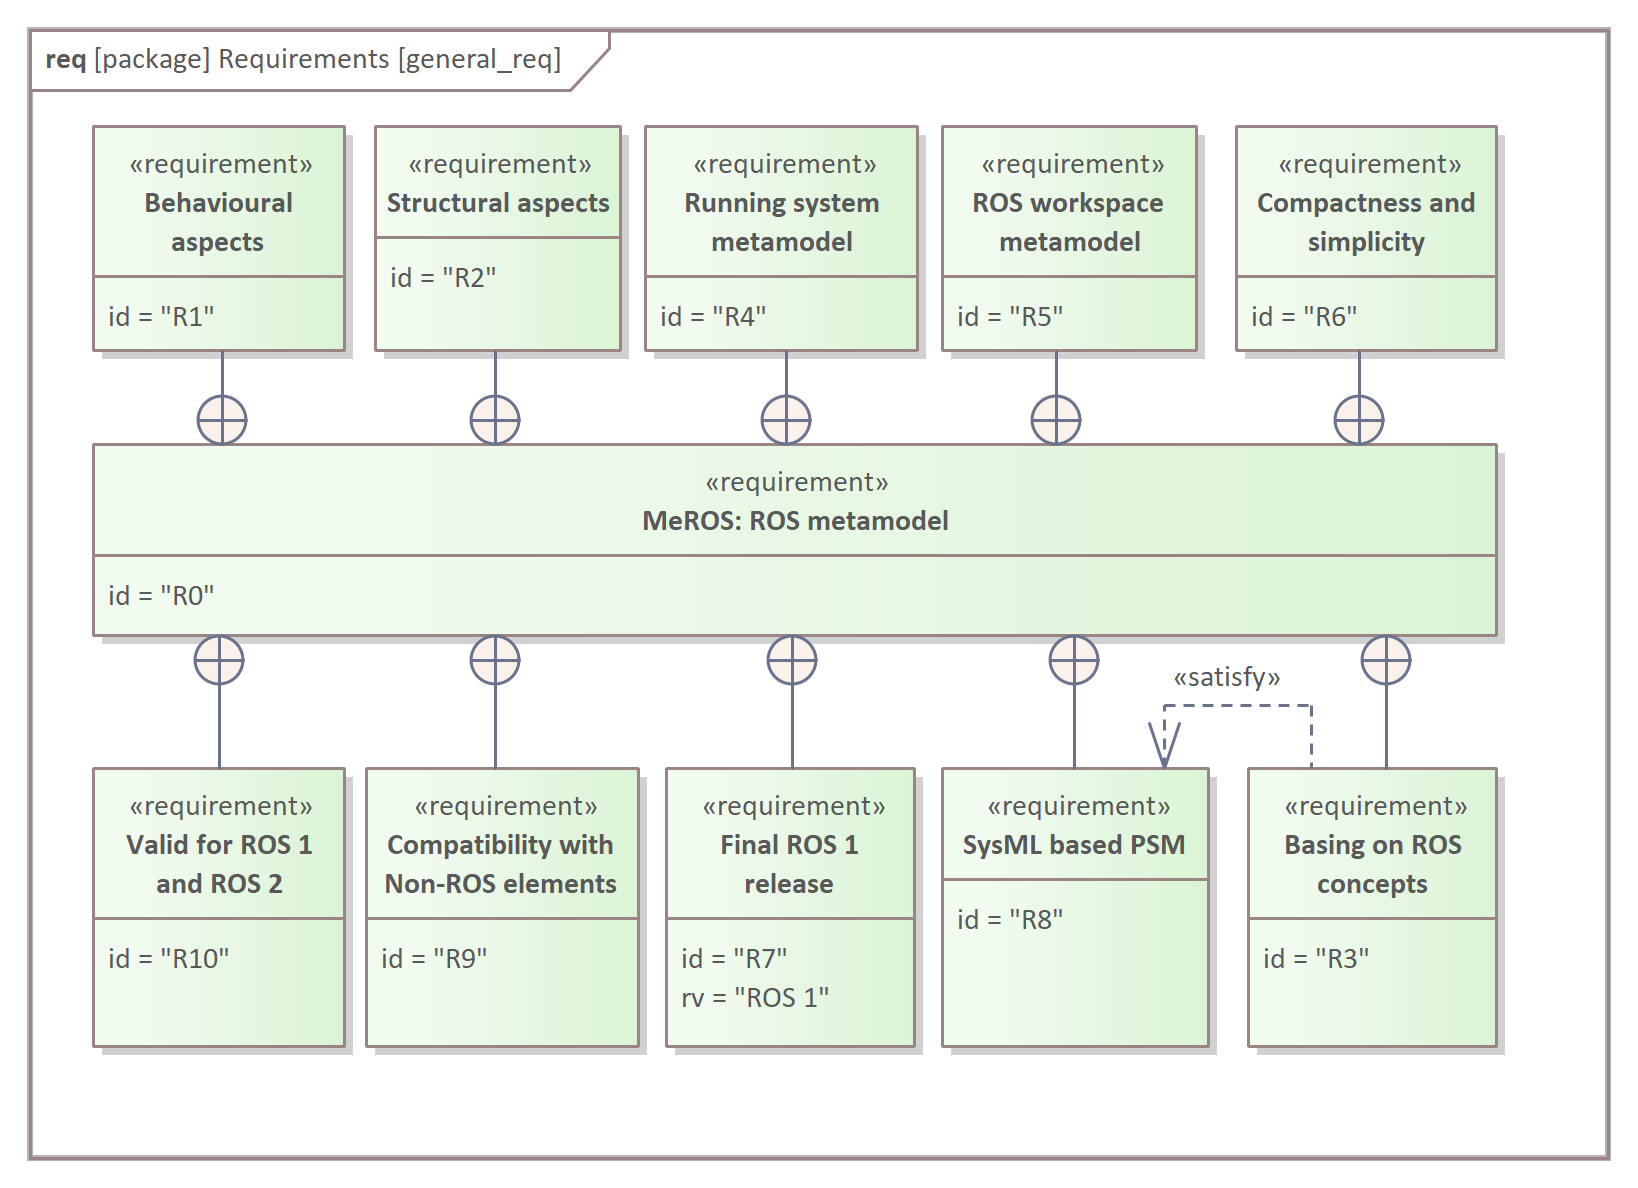
\includegraphics[scale=0.9]{img/requirement_pkg/general_req.png}}
		\end{center}
		\caption{General requirements.} 
		\label{fig:general_req}
	\end{figure}
	
	
	The SysML models have two main parts: behavioural [R1] and structural [R2]. MeROS aims to cover ROS concepts [R3] and not change their labels as long as possible, to maintain conformity and intuitiveness. The ROS system is two-faced. While it is executed [R4], it has a~specific structure and behaviour, but from the developers' point of view, the workspace [R5] is the exposed aspect. The model should be compact and straightforward [R6] rather than unnecessarily elaborate and complicated. One of the assumptions that stand out MeROS from other ROS metamodels is conformity with the final ROS~1 release [R7] (Noetic Ninjemys). Although the SysML-based MeROS is classified into PSM [R8], it should be compatible with Non-ROS elements [R9]. Finally, MeROS metamodel should be valid both for ROS~1 and ROS~2.
	
	The system's structural aspects requirements are presented in Fig.~\ref{fig:structural_aspects_req}.
	
	\begin{figure}[H]
		\centering
		\begin{center}
			{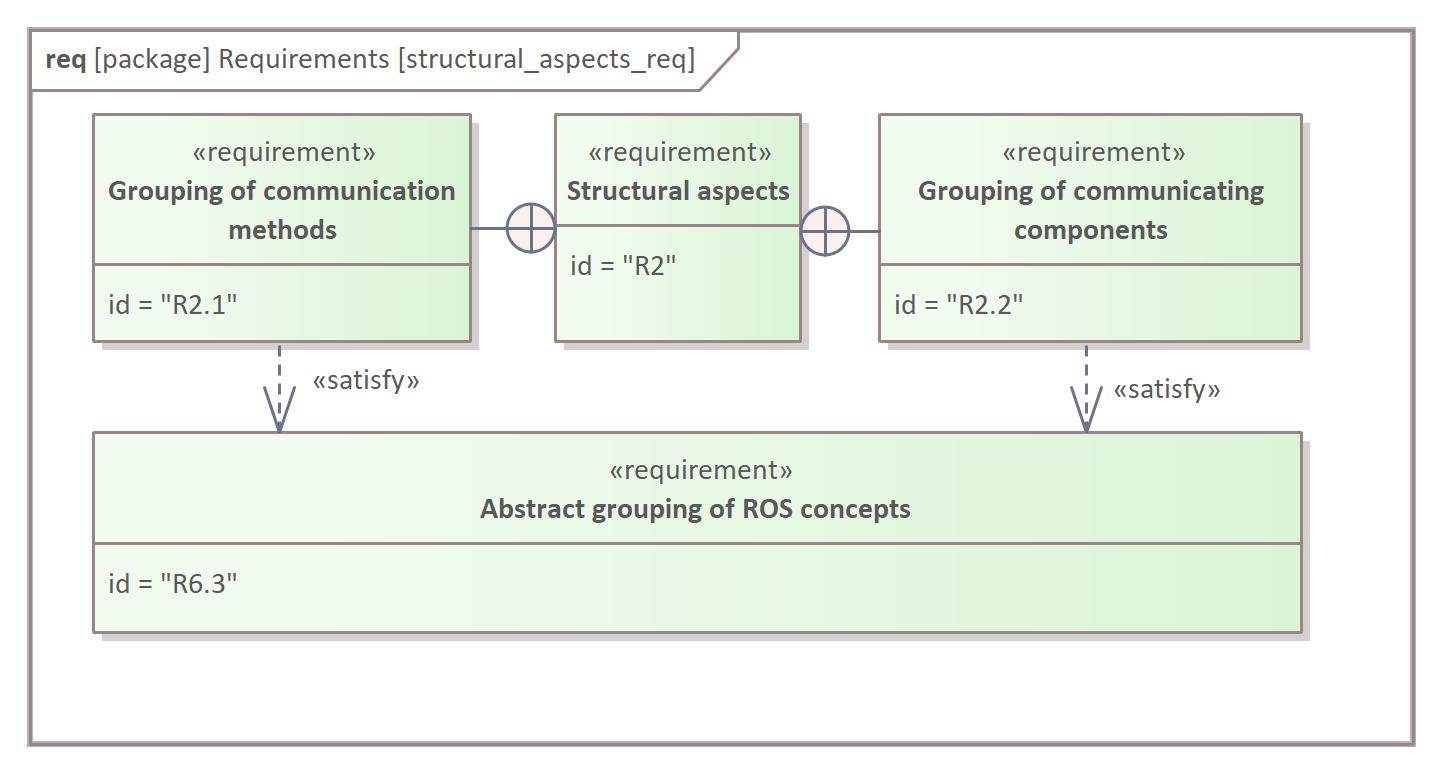
\includegraphics[scale=0.9]{img/requirement_pkg/structural_aspects_req.png}}
		\end{center}
		\caption{Structural aspects requirements.} 
		\label{fig:structural_aspects_req}
	\end{figure}
	
	A~vital addition to the original ROS concepts is the abstract grouping of: (i) communicating methods [R2.1] and (ii) communicating components [R2.2]. The motivation for the introduction of these aggregates is presented further on. It should be noted that several ROS concepts group other concepts in a particular way, especially to deploy the system. Action aggregates Topics and Services (in ROS~2), ROS~1 Node aggregates Nodelets, and ROS~2 Component Container aggregates Nodes.
	The ROS concepts that MeROS models are organised into four major classes (Fig.~\ref{fig:ros_concepts_req}): (i) Communicating components [R3.1], (ii) Communication methods [R3.2], (iii) Workspace [R3.3], and (iv) Other [R3.4].
	

	\begin{figure}[H]
		\centering
		\begin{center}
			{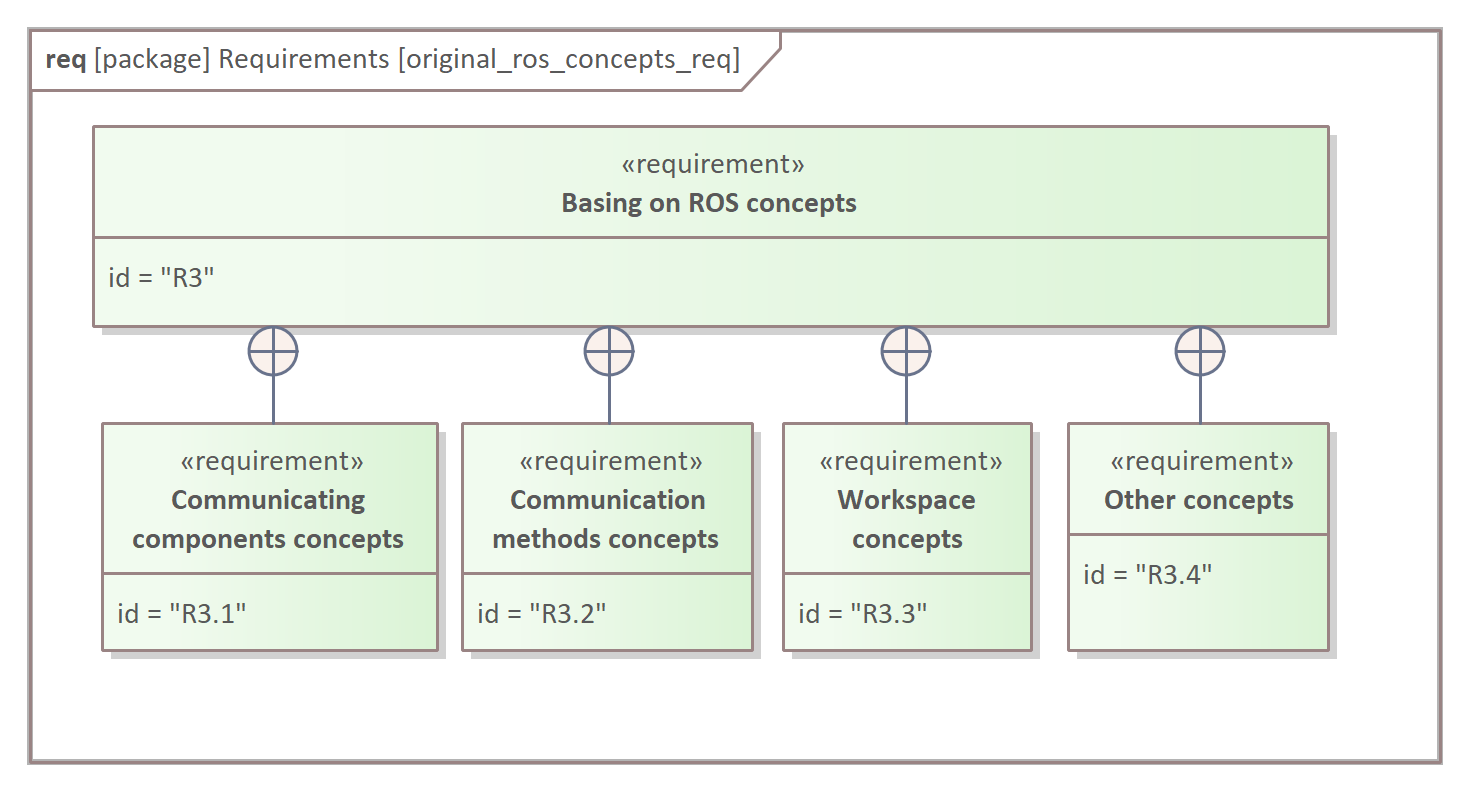
\includegraphics[scale=1.1]{img/requirement_pkg/original_ros_concepts_req.png}}
		\end{center}
		\caption{ROS concepts requirements.} 
		\label{fig:ros_concepts_req}
	\end{figure}
	
	Communicating components [R3.1] are: (i) ROS Node, (ii) ROS Nodelet, (iii) ROS plugin, and (iv) ROS library. Both plugin and library let to share the same code between various Nodes or ROS~1 specific Nodelets. Two ROS nodes are mandatory to execute the ROS~1 system: (i) ROS Master and (ii) rosout.

	\begin{figure}[H]
		\centering
		\begin{center}
			{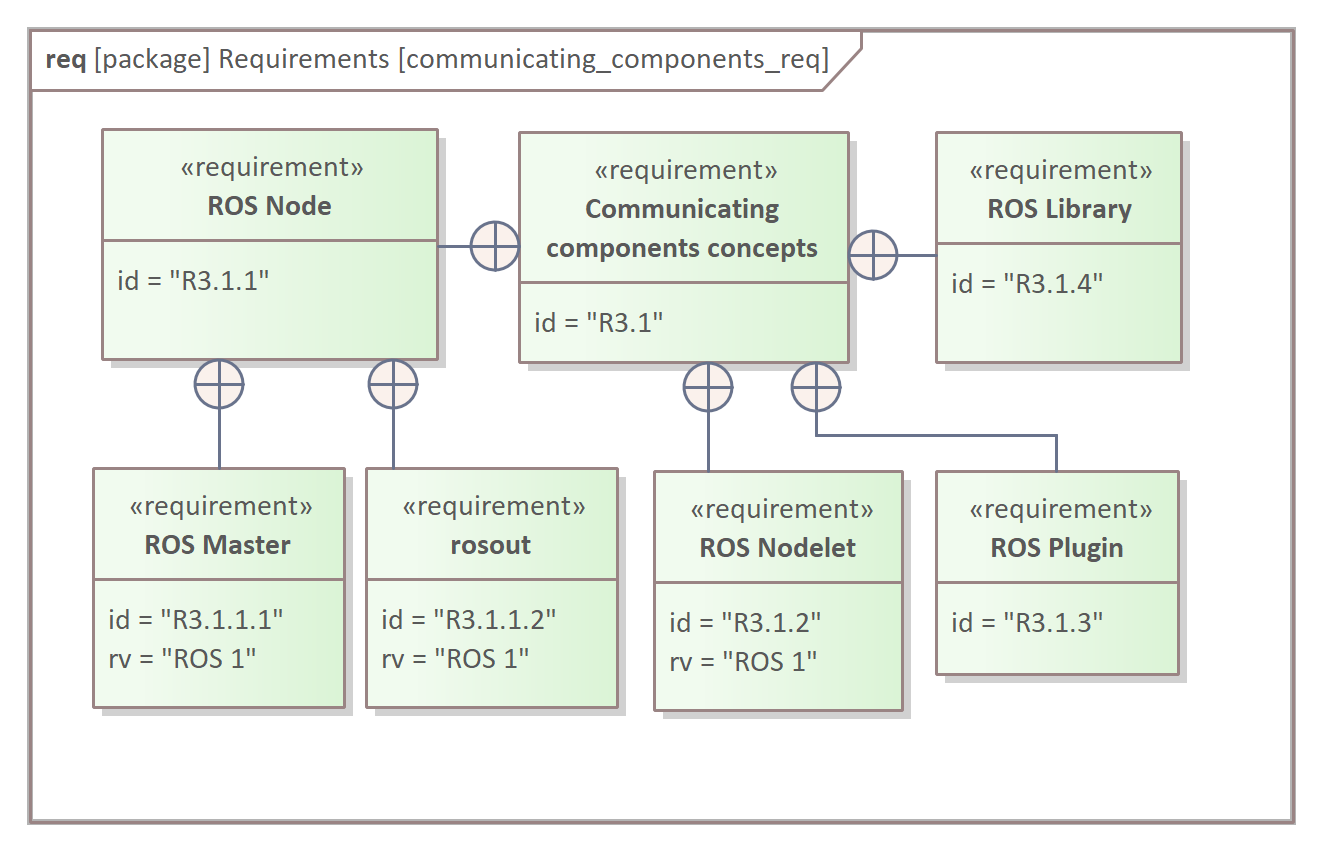
\includegraphics[scale=1]{img/requirement_pkg/communicating_components_req.png}}
		\end{center}
		\caption{Communicating components requirements.} 
		\label{fig:communicating_components_req}
	\end{figure}
	Communication methods are depicted in Fig.~\ref{fig:communication_concepts_req}.
	 Three methods of communication are considered [R3.2] with their inter-component connections and data structures: (i) ROS Topic, its Message and connection, (ii) ROS Service comprising data structure and connection, and finally (iii) ROS Action including data structure and connection.
	
	\begin{figure}[H]
		\centering
		\begin{center}
			{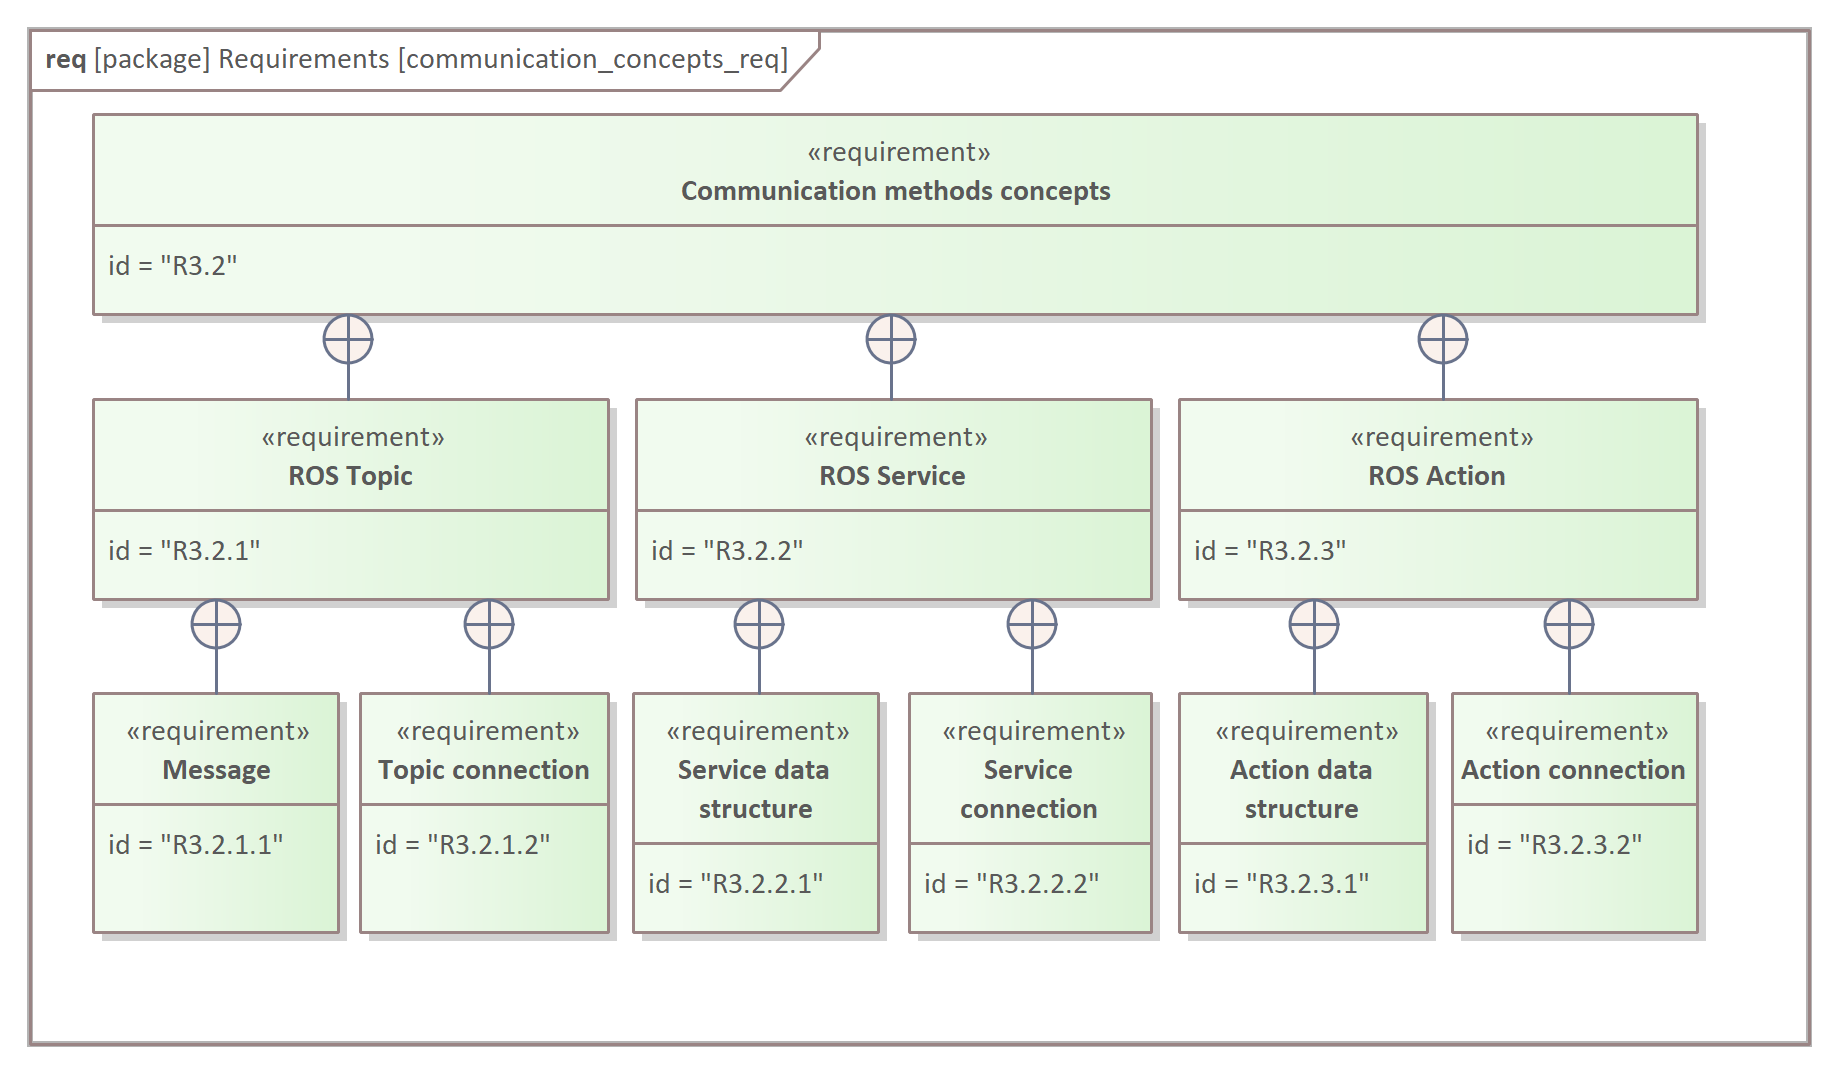
\includegraphics[scale=1]{img/requirement_pkg/communication_concepts_req.png}}
		\end{center}
		\caption{Communication concepts requirements.} 
		\label{fig:communication_concepts_req}
	\end{figure}
	Workspace concept [R3.3] comprises: (i) ROS Package [R3.3.1], (ii) Metapackage [R3.3.2] introduced in the latest releases of ROS~1, (iii) Group of packages [R3.3.3], (iv) Repository [R3.3.4] and (v) ROS Workspace [R3.3.5].
	
	\begin{figure}[H]
		\centering
		\begin{center}
			{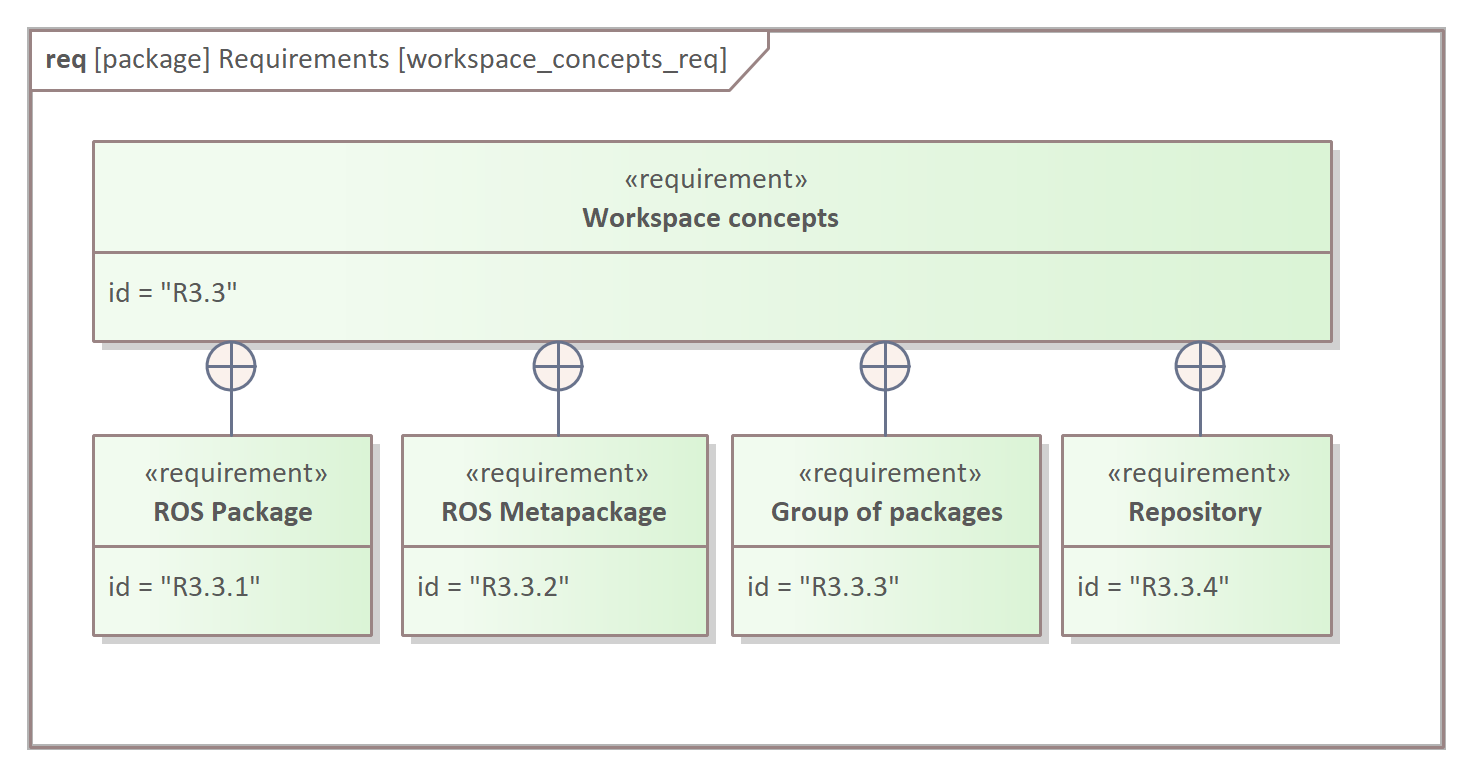
\includegraphics[scale=1]{img/requirement_pkg/workspace_concepts_req.png}}
		\end{center}
		\caption{Workspace concepts requirements.} 
		\label{fig:workspace_concepts_req}
	\end{figure}
	
	\pagebreak
	
	Other concepts (Fig.~\ref{fig:other_concepts_req}) [R3.4] include four elements: (i) ROS Parameter Server manages (ii) ROS Parameters, (iii) roscore forms a collection of programs and nodes that are pre-requisites of a ROS~1-based system. Finally, (iv) ROS Namespace reflects the ROS concept to organise nodes and communication connections. Both ROS Master and rosout are executed with roscore. ROS Parameter Server is a part of ROS Master.
	
	\begin{figure}[H]
			\centering
			\begin{center}
					{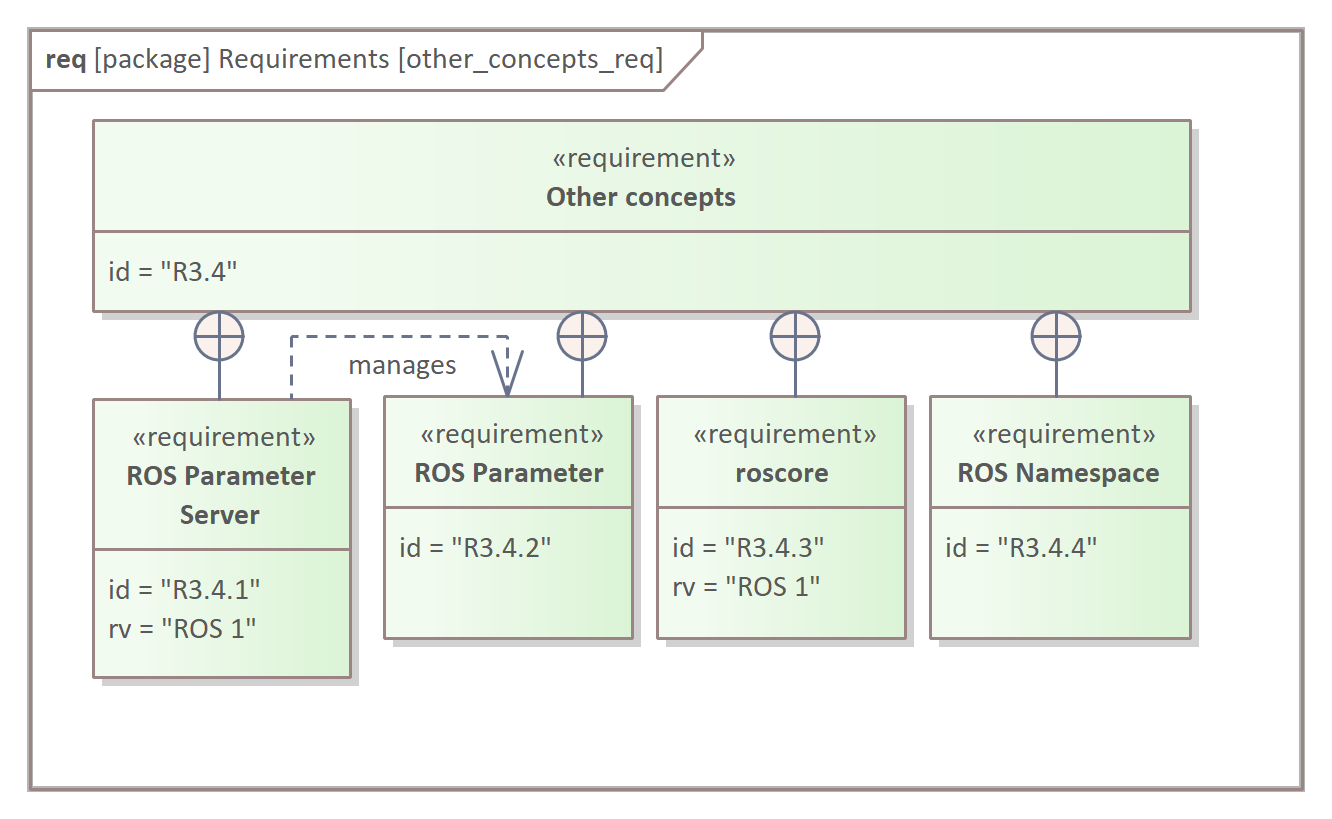
\includegraphics[scale=1.1]{img/requirement_pkg/other_concepts_req.png}}
				\end{center}
			\caption{Other ROS concepts requirements.} 
			\label{fig:other_concepts_req}
		\end{figure}

	Fig.~\ref{fig:roscore_req} presents additional roscore-related relations.


	\begin{figure}[H]
		\centering
		\begin{center}
			{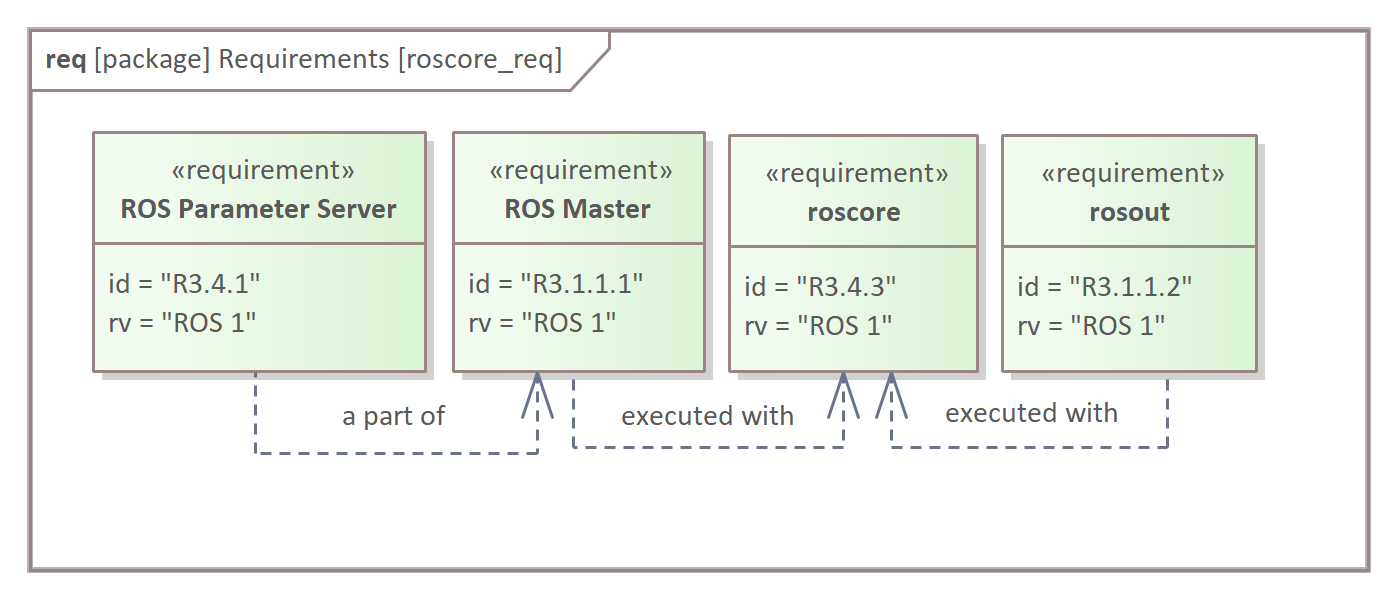
\includegraphics[scale=1.1]{img/requirement_pkg/roscore_req.png}}
		\end{center}
		\caption{roscore related requirements dependences.} 
		\label{fig:roscore_req}
	\end{figure}
	
	\pagebreak
	
	To achieve intuitiveness, MeROS presents a Running system structure (Fig.~\ref{fig:running_system_req}) following ROS rqt\_graph pattern [R4.1]. In particular, there are two ways to visualise communication, including [R4.1.1] and without [R4.1.2]
	dedicated communication components.
	\begin{figure}[H]
		\centering
		\begin{center}
			{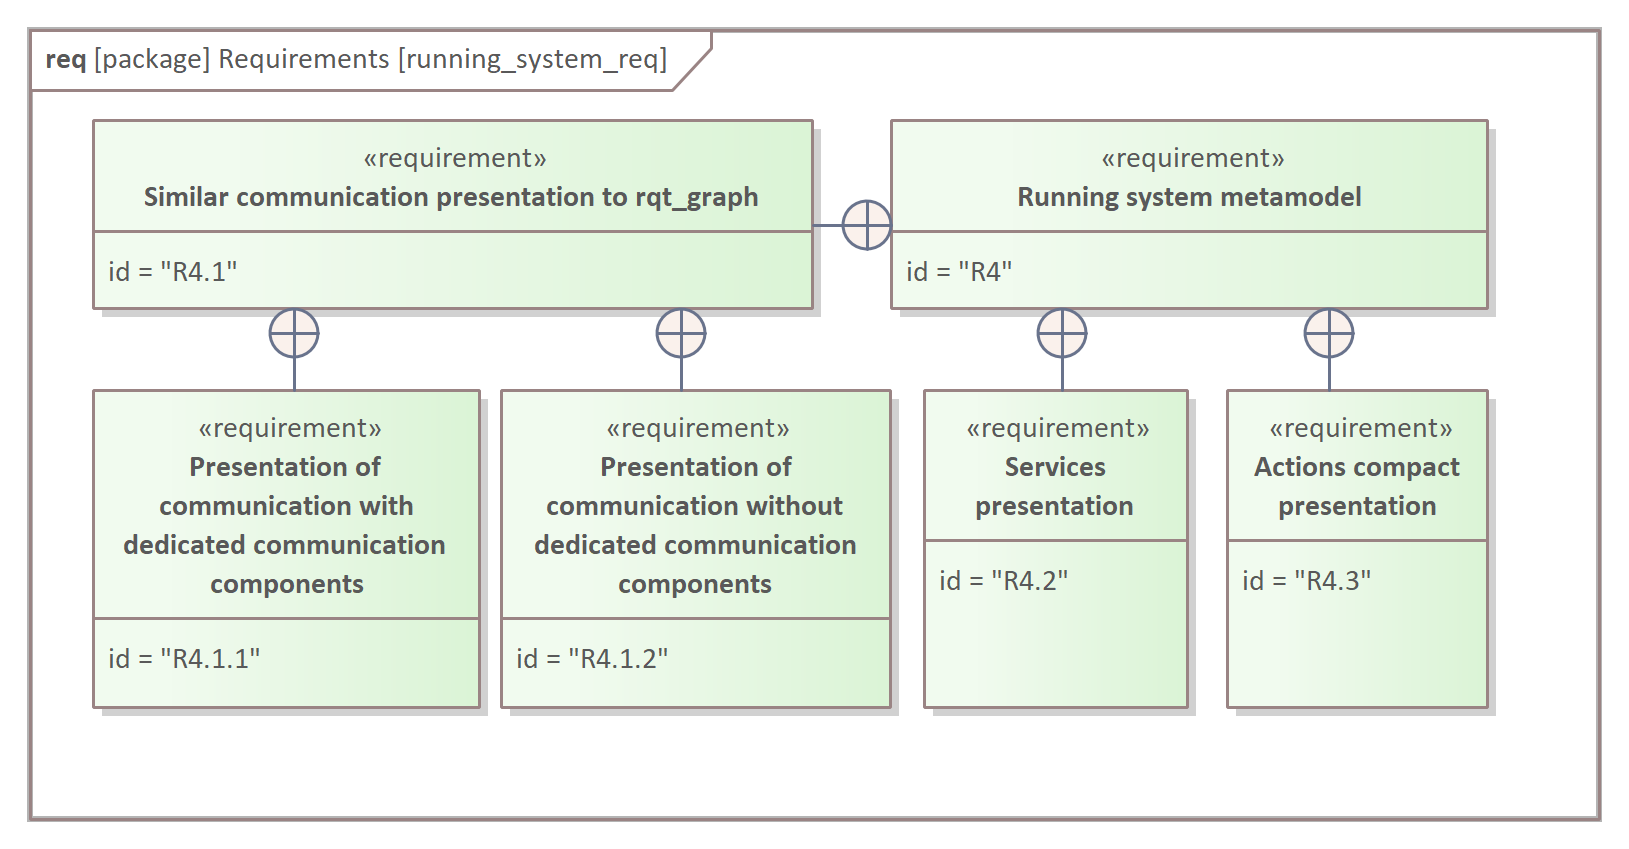
\includegraphics[scale=0.9]{img/requirement_pkg/running_system_req.png}}
		\end{center}
		\caption{Running system requirements.} 
		\label{fig:running_system_req}
	\end{figure}
	 The dedicated components are especially useful in the presentation when many communication components use the same topic both on the publisher and the subscriber side. In opposition, the expression of topic names on arrows connecting communicating components, i.e., without dedicated communication components, let to reduce the number of components needed to depict communication for many topics and a~low number of communicating components. The other advantage of using dedicated communication components is that the particular connection can be split into several diagrams (e.g. ibd (internal block diagram) or sd (sequence diagram)), where the same object represents this connection in every associated diagram. Services [R4.2] and actions [R4.3] should be depicted as an addition to the presentation of the particular topics. It should be noted that rqt\_graph represents actions as a~number of topics and services. In MeROS, the topics and services being part of an action can be aggregated, which reduces the number of depicted connections.
		
			
	The compactness and simplicity [R6] and its nesting requirements are presented in Fig.~\ref{fig:compactness_and_simplicity_req}. 
	
	\begin{figure}[H]
		\centering
		\begin{center}
			{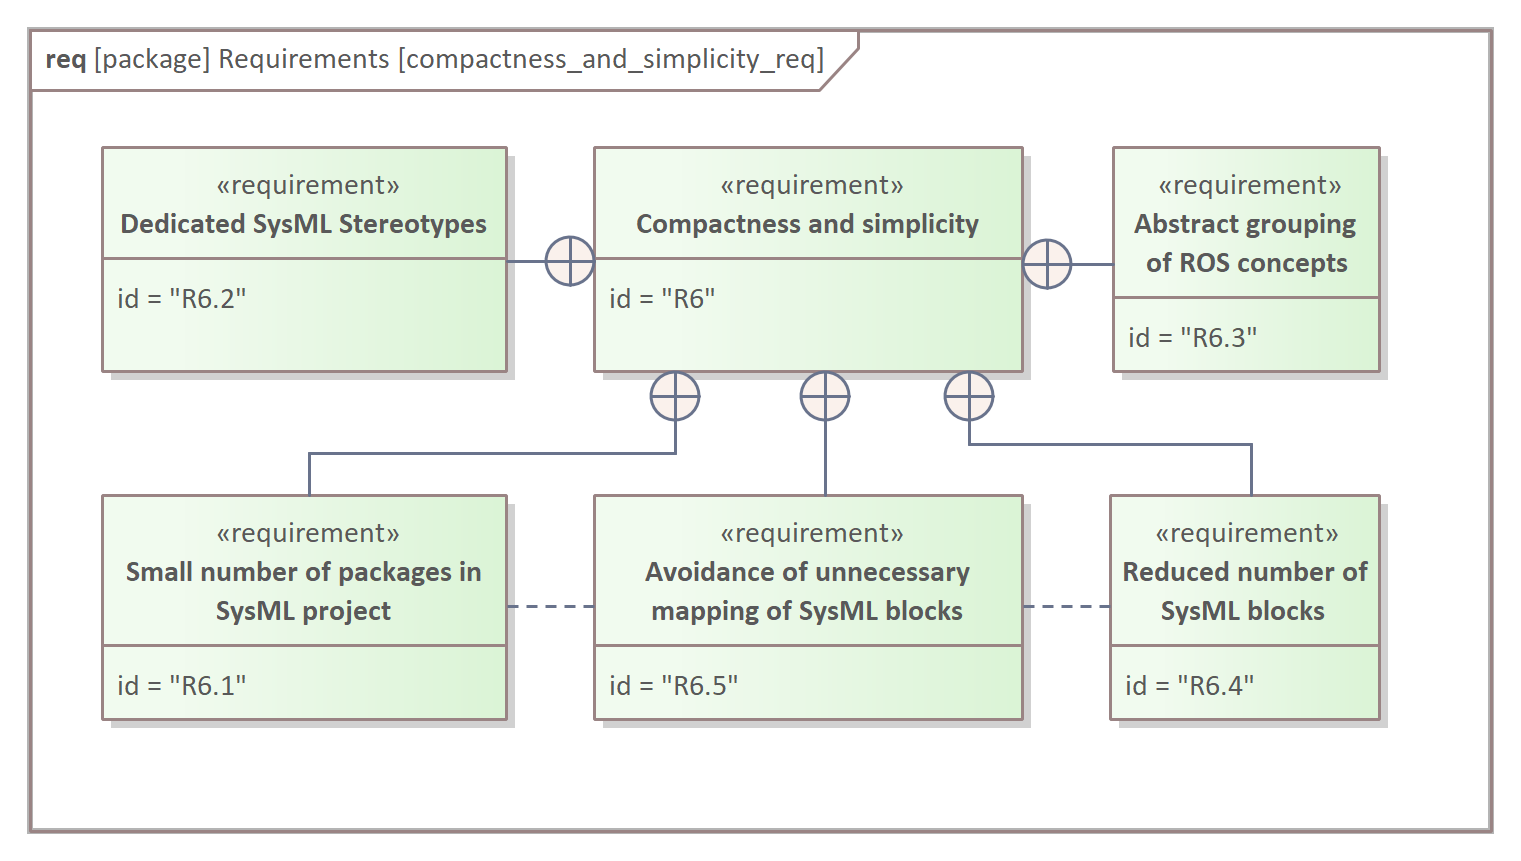
\includegraphics[scale=0.9]{img/requirement_pkg/compactness_and_simplicity_req.png}}
		\end{center}
		\caption{Compactness and simplicity requirements.} 
		\label{fig:compactness_and_simplicity_req}
	\end{figure}
	
	A SysML project to develop and represent MeROS metamodel should consist of a~small number of packages [R6.1], but still, the packages should distinguish the major aspects of development process: (i) metamodel requirements formulation, (ii) metamodel itself, and (iii) metamodel realizations/applications.
	Dedicated SysML stereotypes [R6.2] are introduced to MeROS to replace the direct block specialization representation on diagrams and improve the legibility and compactness of diagrams.
	The grouping of concepts [R6.3] has diverse aims. It enables the presentation of the system part in a~general, PIM-like abstract way, on the logical level rather than a~detailed, PSM-like implementation one. The aggregation reduces the number of objects represented on the diagram to highlight the essential aspects and stay compact and consistent in presentation.
	The number of SysML blocks should be reduced to a reasonable level [R6.4]. Both [R6.1] and [R6.4] help in the Avoidance of unnecessary mapping of SysML blocks [R6.5].

	There are three elements in the requirements set that satisfy the evolution of the ROS~1  finalised with its ultimate release -- Noetic Ninjemys -- (Fig.~\ref{fig:final_ros1_release_req}): (i) ROS Nodelet  (introduced primarily to increase the efficiency of ROS components switching), (ii) ROS Action , and (iii) ROS Metapackage.
	
	\begin{figure}[H]
		\centering
		\begin{center}
			{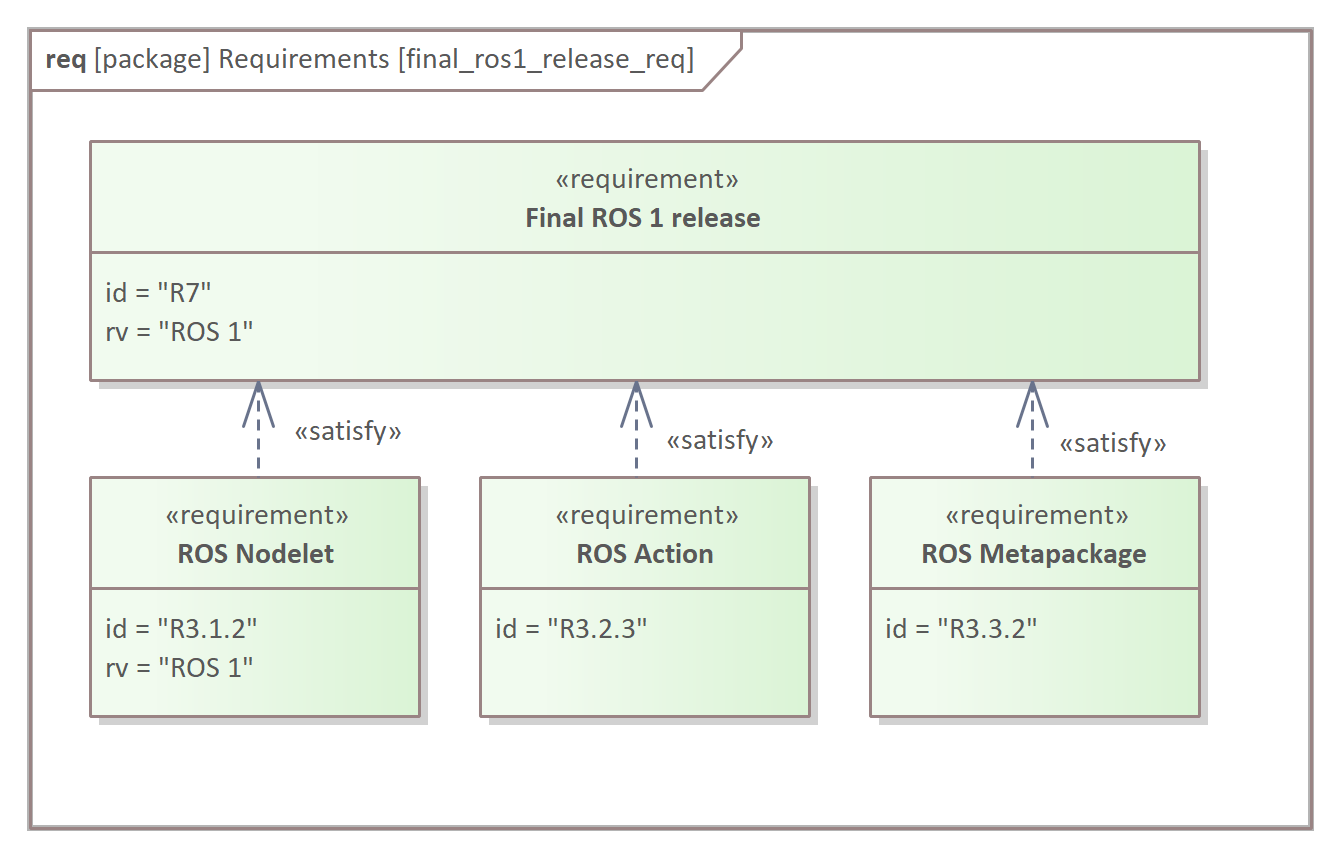
\includegraphics[scale=1.1]{img/requirement_pkg/final_ros1_release_req.png}}
		\end{center}
		\caption{Final ROS 1 release requirements.} 
		\label{fig:final_ros1_release_req}
	\end{figure}
	
	
	
\section{MeROS metamodel}
\label{sec:metamodel}
	
	MeROS metamodel is formulated according to the requirements discussed in the previous section. Sec.~\ref{sec:metamodel-composition} presents MeROS blocks' structural composition, and sec.~\ref{sec:metamodel-communication} describes inter-component communication. From the metamodel perspective, the structural aspects [R2] are formulated in both sections, while behavioural [R1] is in the latter. The diagrams comprise selected requirements being allocated to expose the MeROS metamodel development process. 
	
	The MeROS diagrams were created in the Enterprise Architect development tool within the SysML project [R8] and organised in three packages [R6.1] (Fig.~\ref{fig:meros_project_packages_pkg}): (i) Requirement Model related to requirements formulation and analysis, (ii) MeROS -- the metamodel itself, (iii) Rico Controller -- the exemplary ROS~1 application of MeROS described in sec.~\ref{sec:application-example}. The stereotypes are introduced in MeROS metamodel with the dedicated MeROS profile [R6.2].
	
		
	\begin{figure}[H]
		\centering
		\begin{center}
			{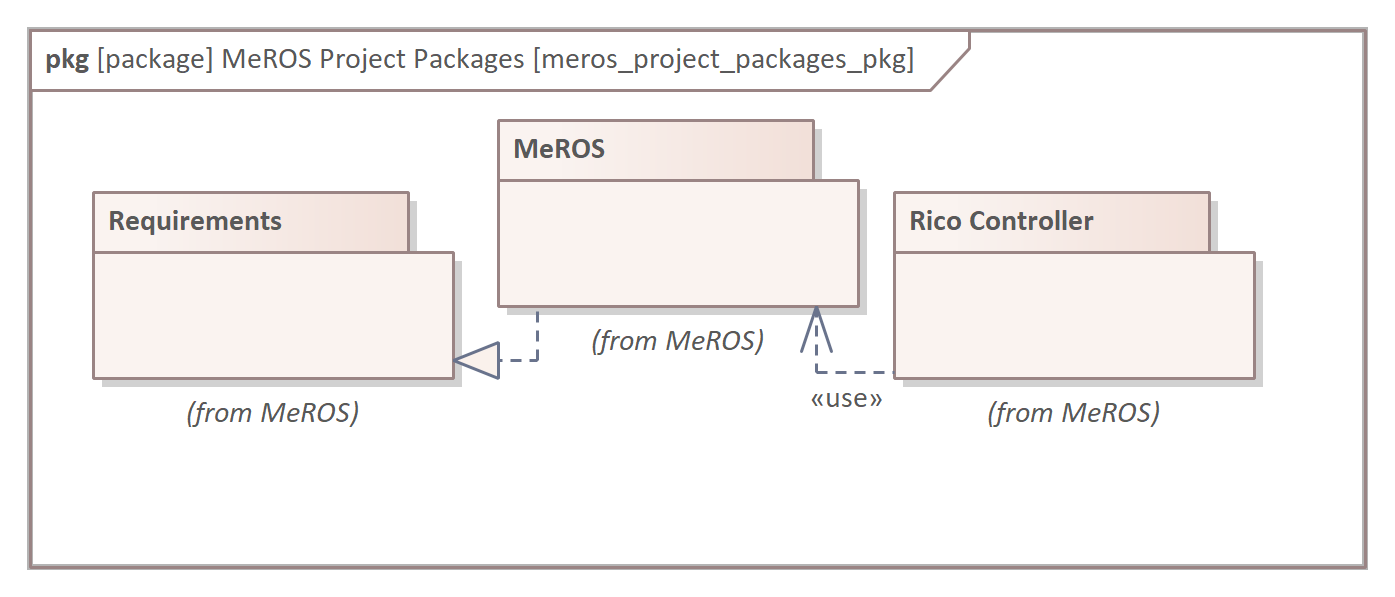
\includegraphics[scale=1.0]{img/meros_project_packages_pkg.png}}
		\end{center}
		\caption{MeROS project SysML packages, where Rico Controller is an exemplary realisation of MeROS metamodel.} 
		\label{fig:meros_project_packages_pkg}
	\end{figure}
	
\subsection{Metamodel composition}
\label{sec:metamodel-composition}

	The degree of specificity of a metamodel is a compromise between its comprehensiveness (and, therefore, more general formulation) and a more accurate representation of a particular subclass of specific implementations. The metamodel contains compositions of elements and other primary relationships. Attributes and operations range widely, in particular between ROS~1 and ROS~2. Hence, their inclusion would lead to overgrowth and complication of the metamodel [R6]. Models derived from the metamodel can define their operations and new relations specific to a particular system. 
	
	The SysML blocks reflect ROS concepts [R3], and their composition is depicted in bdd (block definition diagrams). The metamodel is formulated in a~single SysML package. Hence, Groups of Packages (especially Workspaces) and Intrasystems are composed into ROS System (Fig.~\ref{fig:ros_system_bdd}). 
	
		
	\begin{figure}[H]
		\centering
		\begin{center}
			{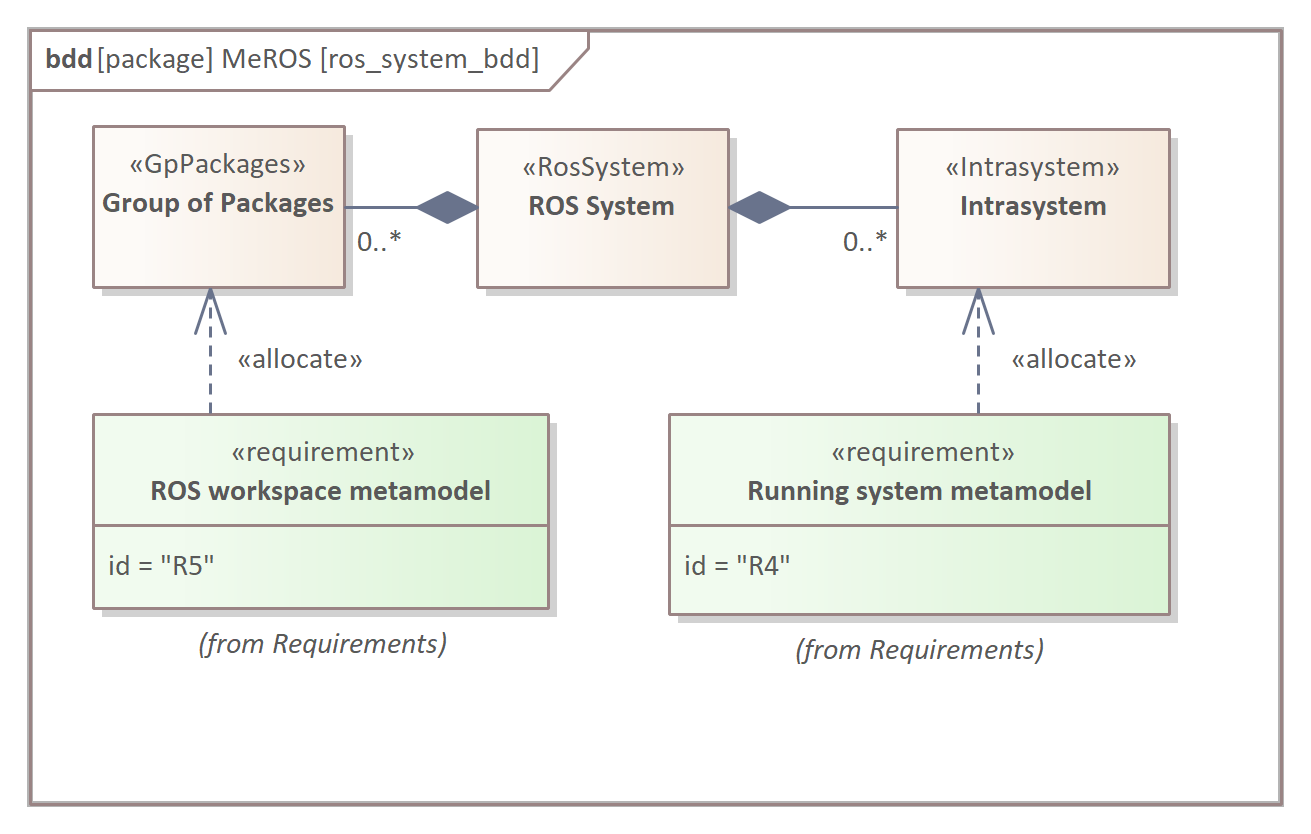
\includegraphics[scale=1.1]{img/meros_pkg/ros_system_bdd.png}}
		\end{center}
		\caption{ROS system general composition -- bdd.} 
		\label{fig:ros_system_bdd}
	\end{figure}
	
	Consequently, some concepts (e.g., Node) occur in Workspaces and Intrasystems. It reduces the number of SysML blocks in the metamodel [R6.4] and eliminates the need for unnecessary mapping of SysML blocks [R6.5].
		
	\pagebreak	
		
	In MeROS, a~Communicating Component (Fig.~\ref{fig:communicating_components_bdd}) is a~crucial abstraction of a~number of ROS concepts to represent their standardised role regarding communication. 
	
		
	\begin{figure}[H]
		\centering
		\begin{center}
			{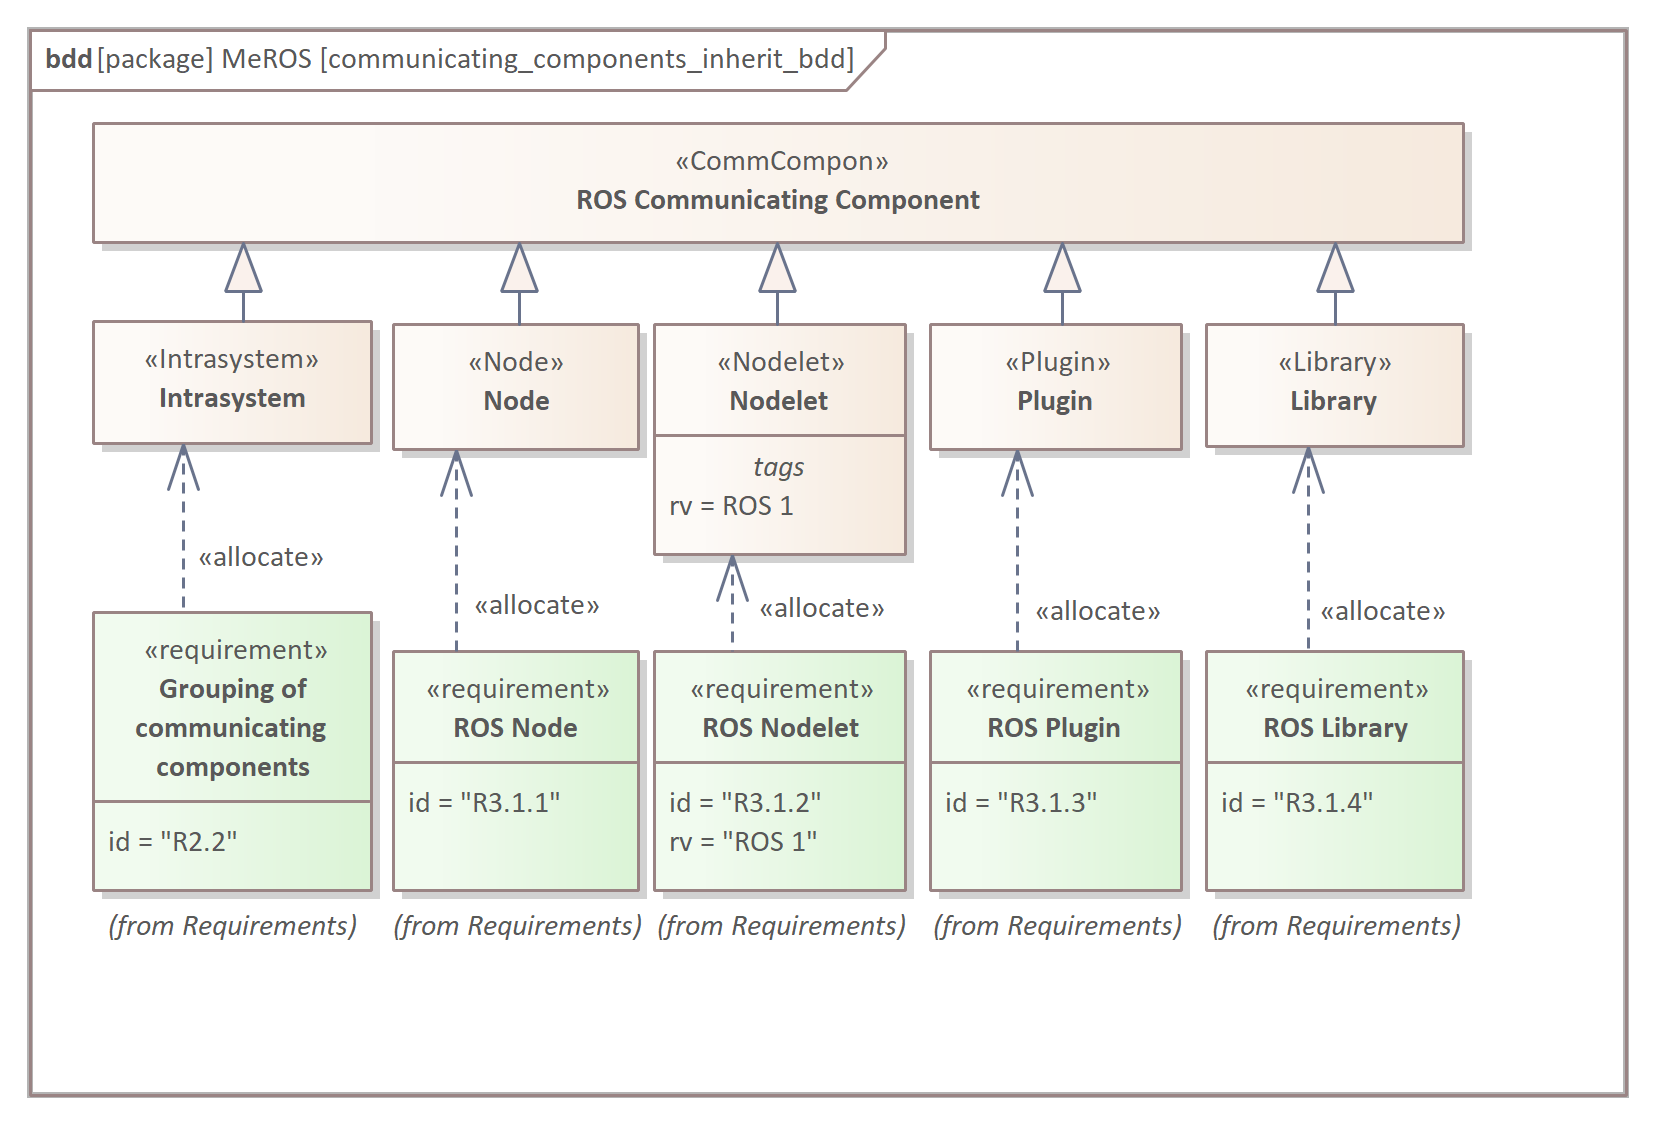
\includegraphics[scale=1]{img/meros_pkg/communicating_components_inherit_bdd.png}}
		\end{center}
		\caption{Communicating Component and specialised blocks -- bdd.} 
		\label{fig:communicating_components_bdd}
	\end{figure}
	
	It should be noted that behavioural aspects of a~particular model specified in MeROS can be formulated by operation specification as an act (activity), sd (sequence), or stm (state machine) diagrams. The Intrasystem is one of the aggregates added to the base ROS concepts in MeROS. 
	
	\pagebreak
	
	For clarity, relations of Communicating Components are depicted in several diagrams. Fig.~\ref{fig:communicating_component_topics_bdd} considers Topics and their Data Structures. Here, the Communicating Component can act as a publisher or a subscriber.	
	 
	
	\begin{figure}[H]
		\centering
		\begin{center}
			{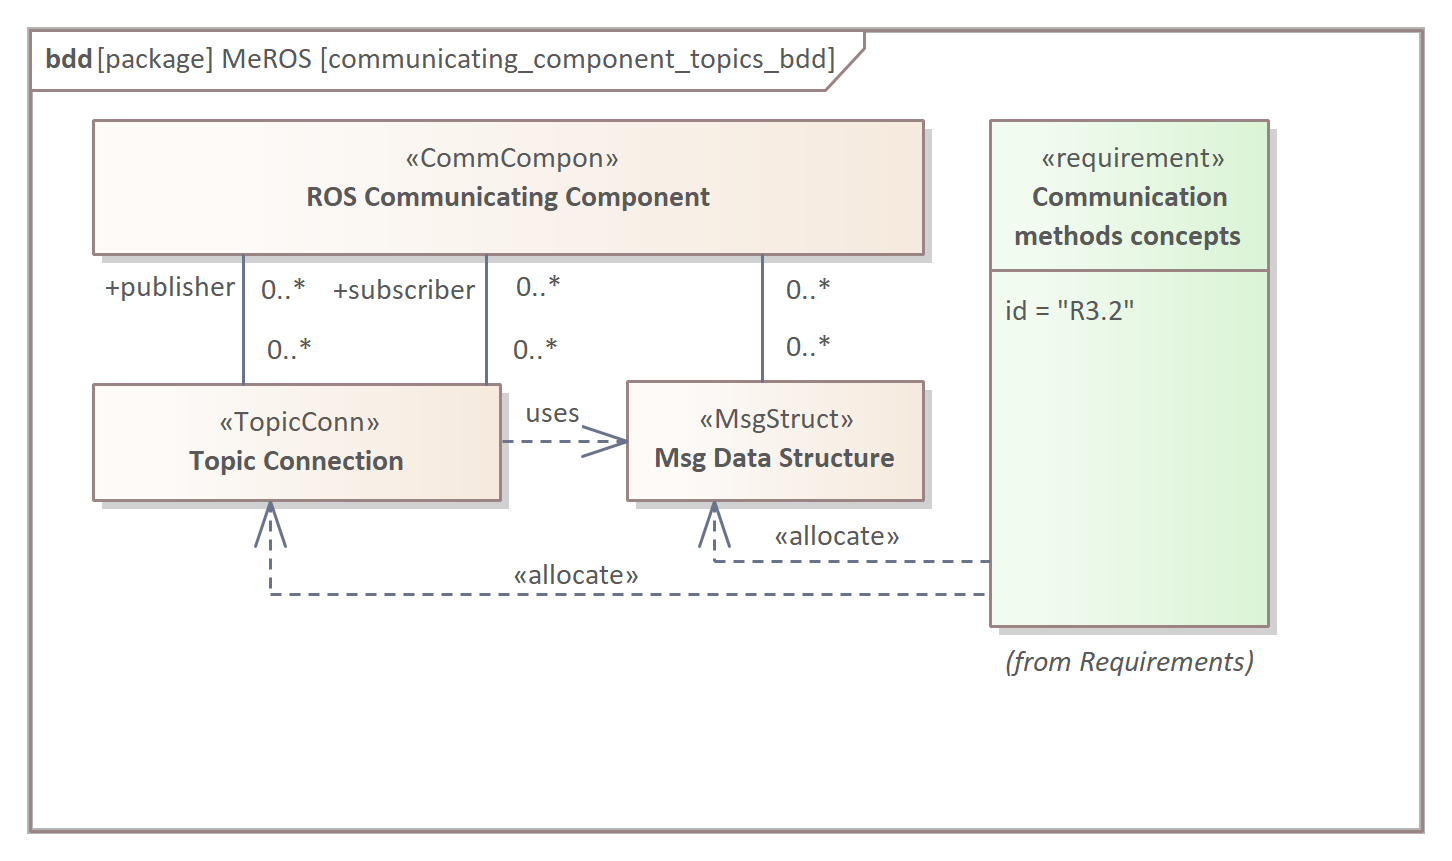
\includegraphics[scale=1.1]{img/meros_pkg/communicating_component_topics_bdd.png}}
		\end{center}
		\caption{Communicating Component relations -- topics -- bdd.} 
		\label{fig:communicating_component_topics_bdd}
	\end{figure}
	
	Fig.~\ref{fig:communication_blocks_services_bdd} depicts Services and their Data Structures. In this case, the Communicating Component can act as a server or a client.	
	
		
	\begin{figure}[H]
		\centering
		\begin{center}
			{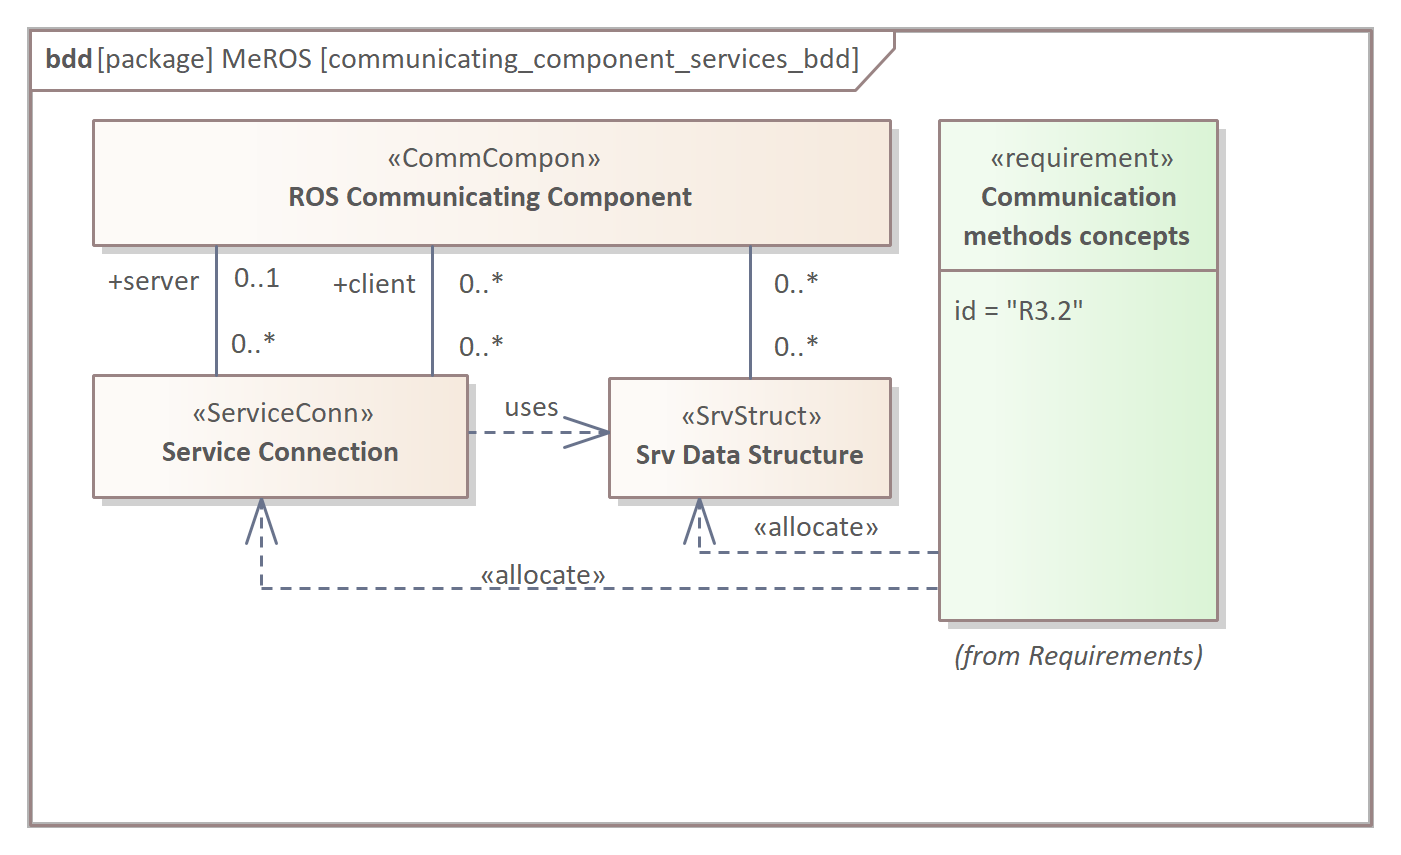
\includegraphics[scale=1.1]{img/meros_pkg/communicating_component_services_bdd.png}}
		\end{center}
		\caption{Communicating Component relations -- services -- bdd.} 
		\label{fig:communication_blocks_services_bdd}
	\end{figure}
	S
	In ROS~2, an Action bases on Topics and Services while in ROS~1 only on Topics. From functional point of view, ROS~1 specific Topics included in Action have their equivalents in ROS~2 specific Services. 
	
	\pagebreak
	
	The Actions are depicted in two diagrams -- Fig.~\ref{fig:communicating_component_actions_bdd} and Fig.~\ref{fig:action_bdd}. Similarly to Services, the Communicating Component can act as a server or a client.	 
	
	
	\begin{figure}[H]
		\centering
		\begin{center}
			{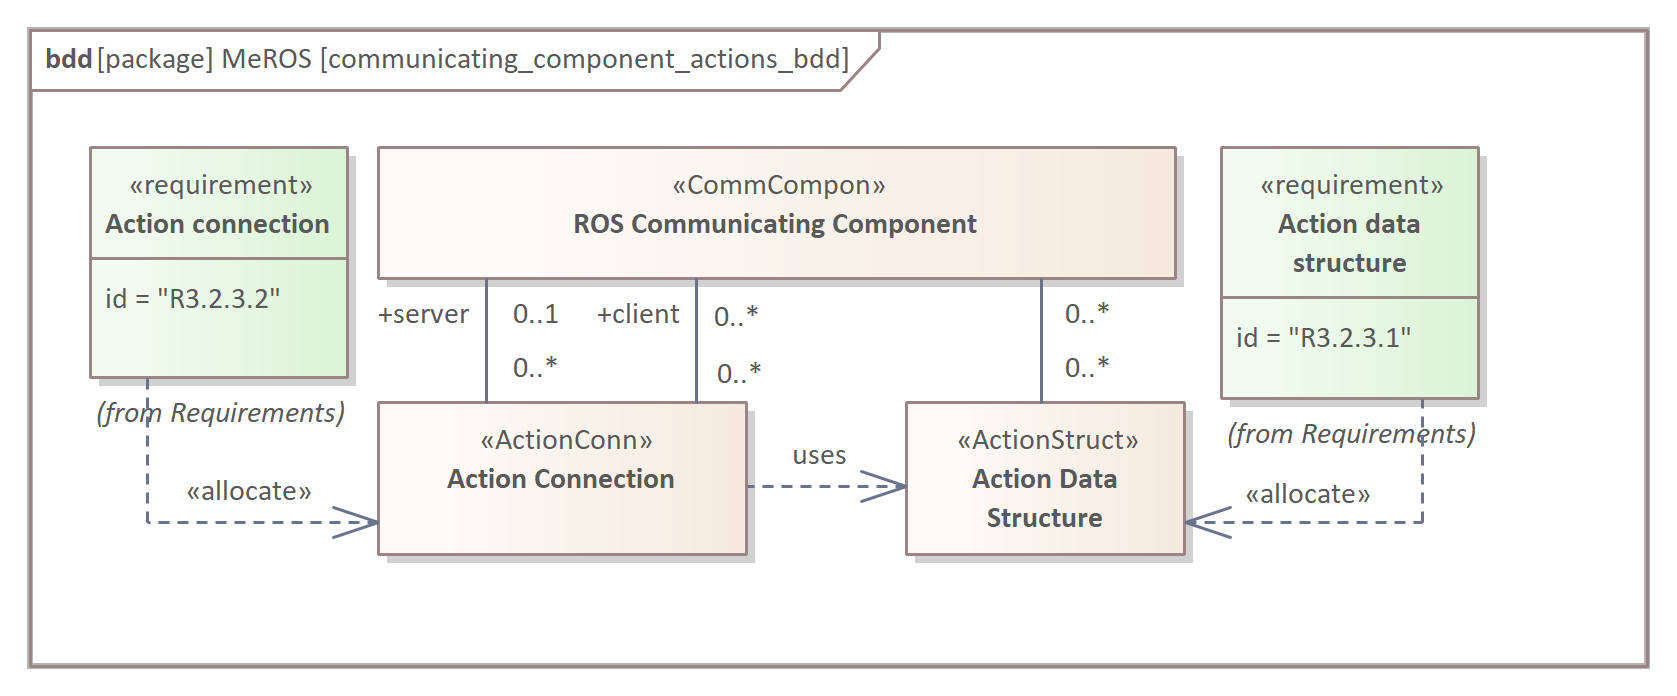
\includegraphics[scale=1]{img/meros_pkg/communicating_component_actions_bdd.png}}
		\end{center}
		\caption{Communicating Component relations -- actions -- bdd.} 
		\label{fig:communicating_component_actions_bdd}
	\end{figure}
	
	\begin{figure}[hbt]
		\centering
		\begin{center}
			{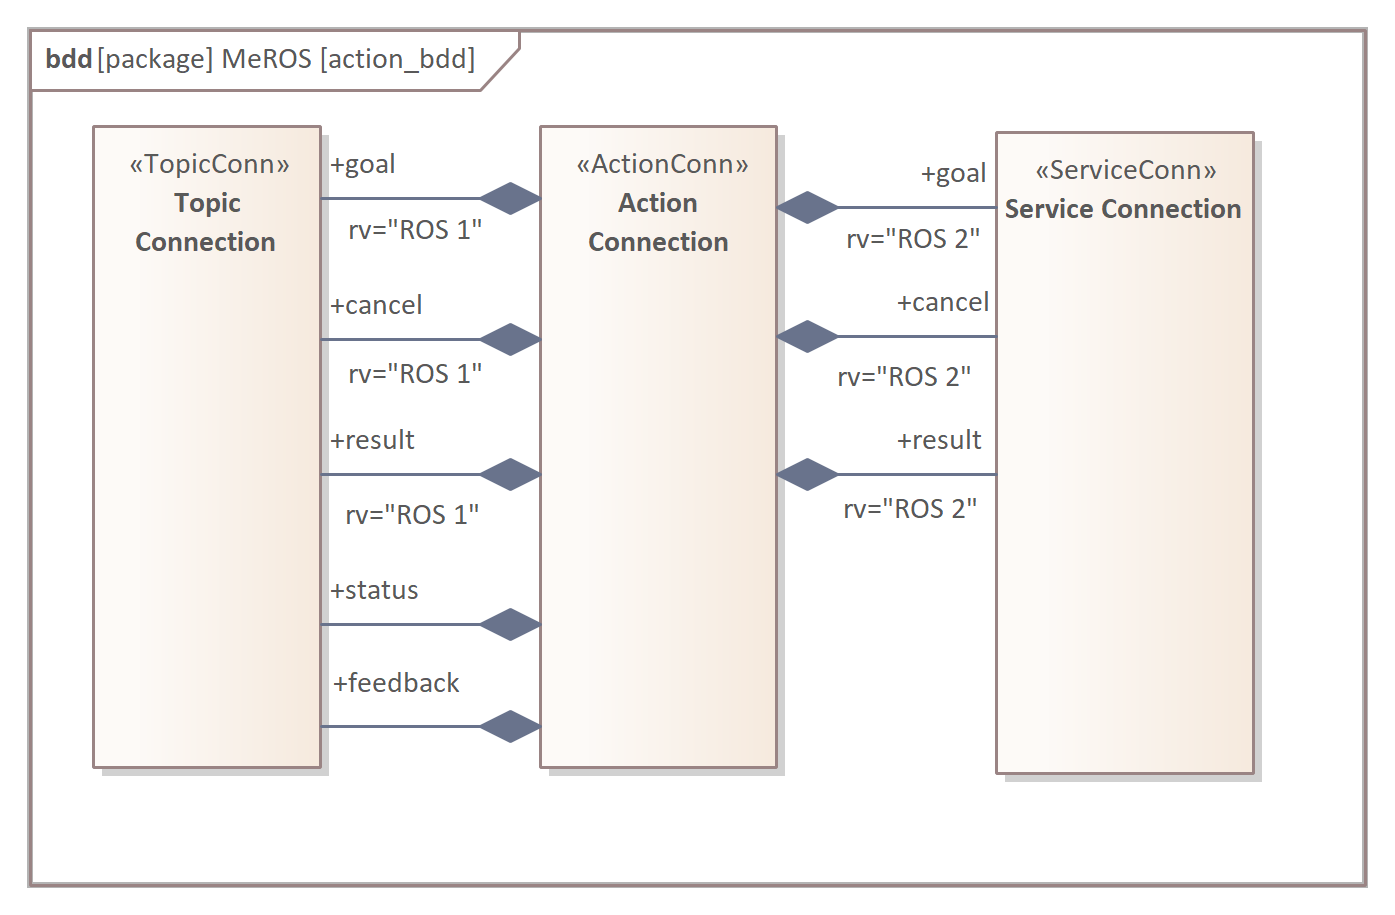
\includegraphics[scale=1.1]{img/meros_pkg/action_bdd.png}}
		\end{center}
		\caption{Action -- bdd.} 
		\label{fig:action_bdd}
	\end{figure}
	
	\pagebreak
	
	Fig.~\ref{fig:communicating_component_other_bdd} describes how Non-ROS elements are taken into account in relation to communication. Additionally, the figure presents Communication Channel relation to ROS Communicating Component.
	

	\begin{figure}[H]
		\centering
		\begin{center}
			{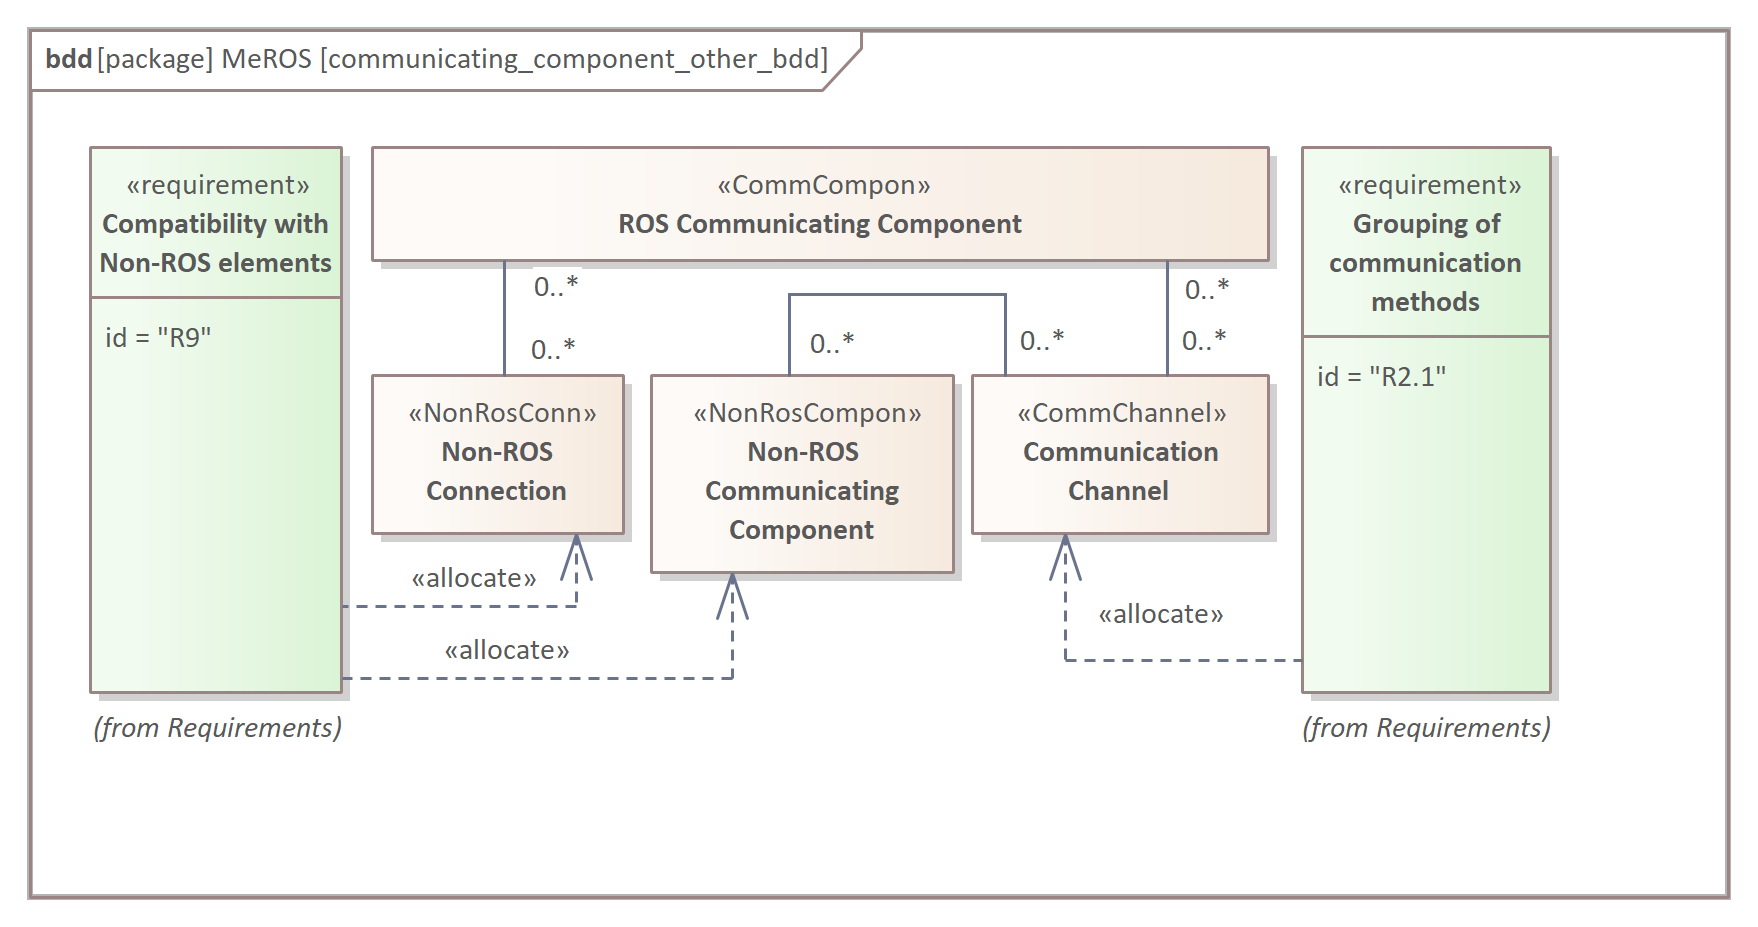
\includegraphics[scale=0.95]{img/meros_pkg/communicating_component_other_bdd.png}}
		\end{center}
		\caption{Communicating Component relations -- aggregates, Non-ROS elements -- bdd.} 
		\label{fig:communicating_component_other_bdd}
	\end{figure}
	
	Besides standard ROS communication methods, the Non-ROS are also included (e.g., http request) to achieve interfaces with Non-ROS parts of the general system. An Action Data Structure comprises data used by three of five Topics composed in Action, i.e., goal, feedback and result. Two remaining Topics, i.e., cancel and status are standardised.
	
	 The Communication Channel \cite{palka2022communication} concept depicted in Fig.~\ref{fig:communication_channel_bdd} is introduced to aggregate specializations of ROS connection (Topic connections, Service connections, and Action connections) as well as Non-ROS Connections. The Communication Channel can also aggregate different Communication Channels.
	 
  
 	\begin{figure}[H]
	 	\centering
	 	\begin{center}
	 		{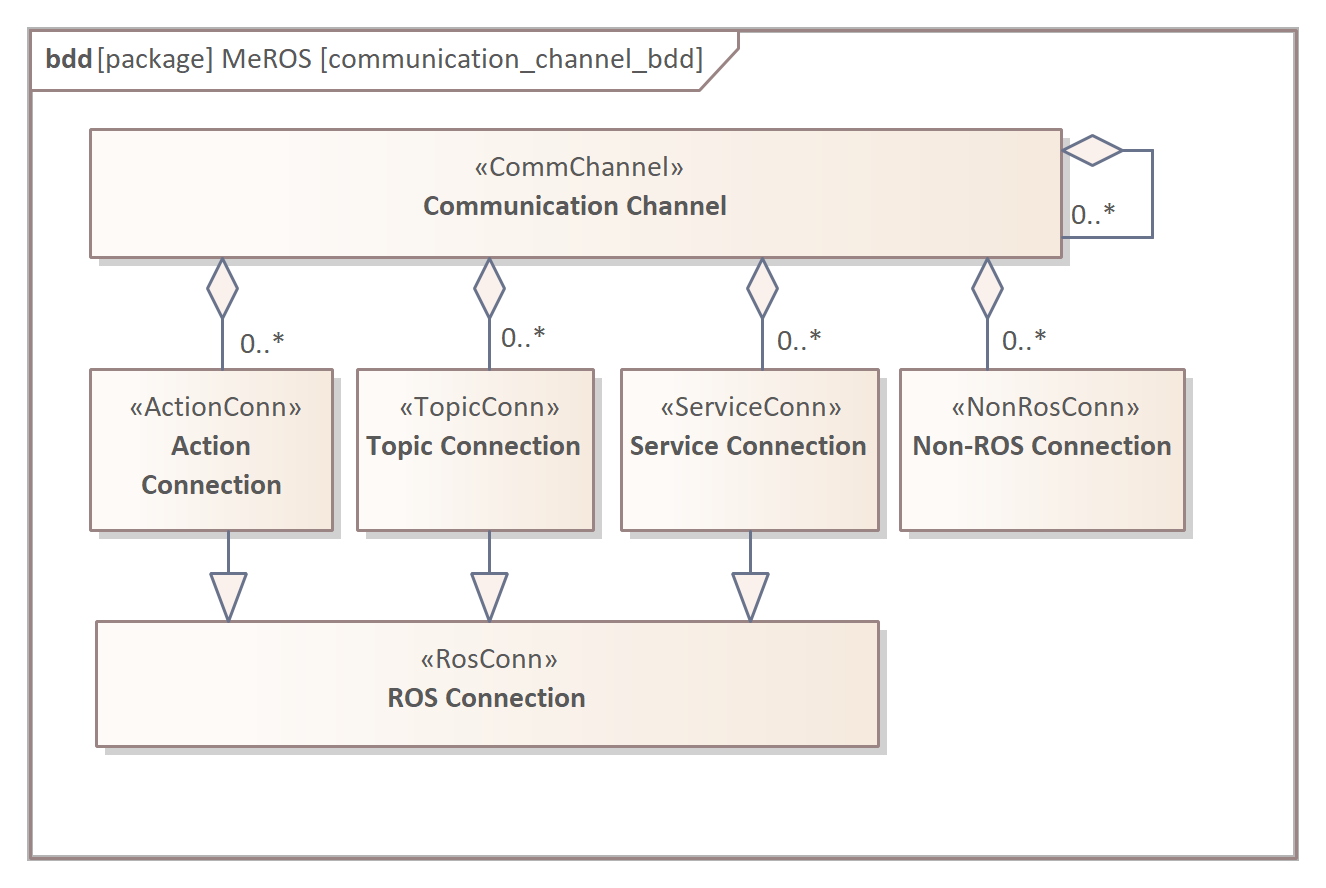
\includegraphics[scale=0.95]{img/meros_pkg/communication_channel_bdd.png}}
	 	\end{center}
	 	\caption{Communication Channel -- bdd.} 
	 	\label{fig:communication_channel_bdd}
	 \end{figure}
	 
 	The Node (Fig.~\ref{fig:node_bdd}) composes Parameters and Nodelets (the latter in ROS~1). Two specific Nodes are considered in the metamodel: ROS Master and rosout. In ROS~2, Component Container aggregates Nodes executed in a single process.
 	
	 
 	\begin{figure}[H]
	 	\centering
	 	\begin{center}
	 		{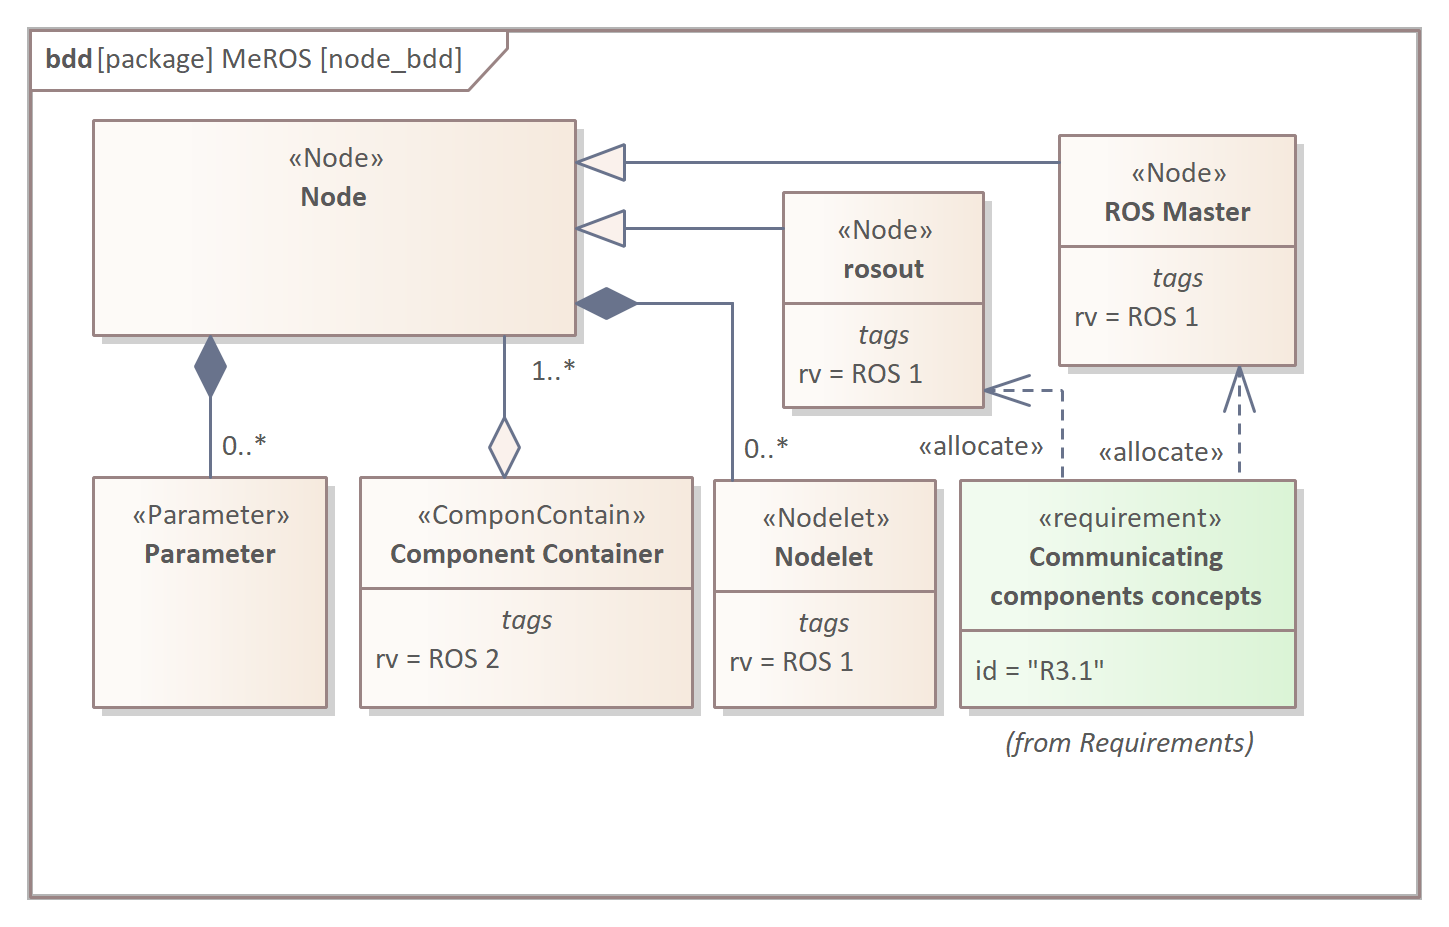
\includegraphics[scale=1.0]{img/meros_pkg/node_bdd.png}}
	 	\end{center}
	 	\caption{Node -- bdd.} 
		 	\label{fig:node_bdd}
	 \end{figure}
	 
	The Intrasystem (Fig.~\ref{fig:intrasystem_bdd}) composes ROS and Non-ROS Communicating Component specializations as well as Connections between them. A Parameter block is introduced also for ROS~1. In ROS~2, due to safety reasons, Parameter is composed only into Nodes. Optionally Intrasystem composes the other Intrasystems.
	

	\begin{figure}[H]
		\centering
		\begin{center}
			{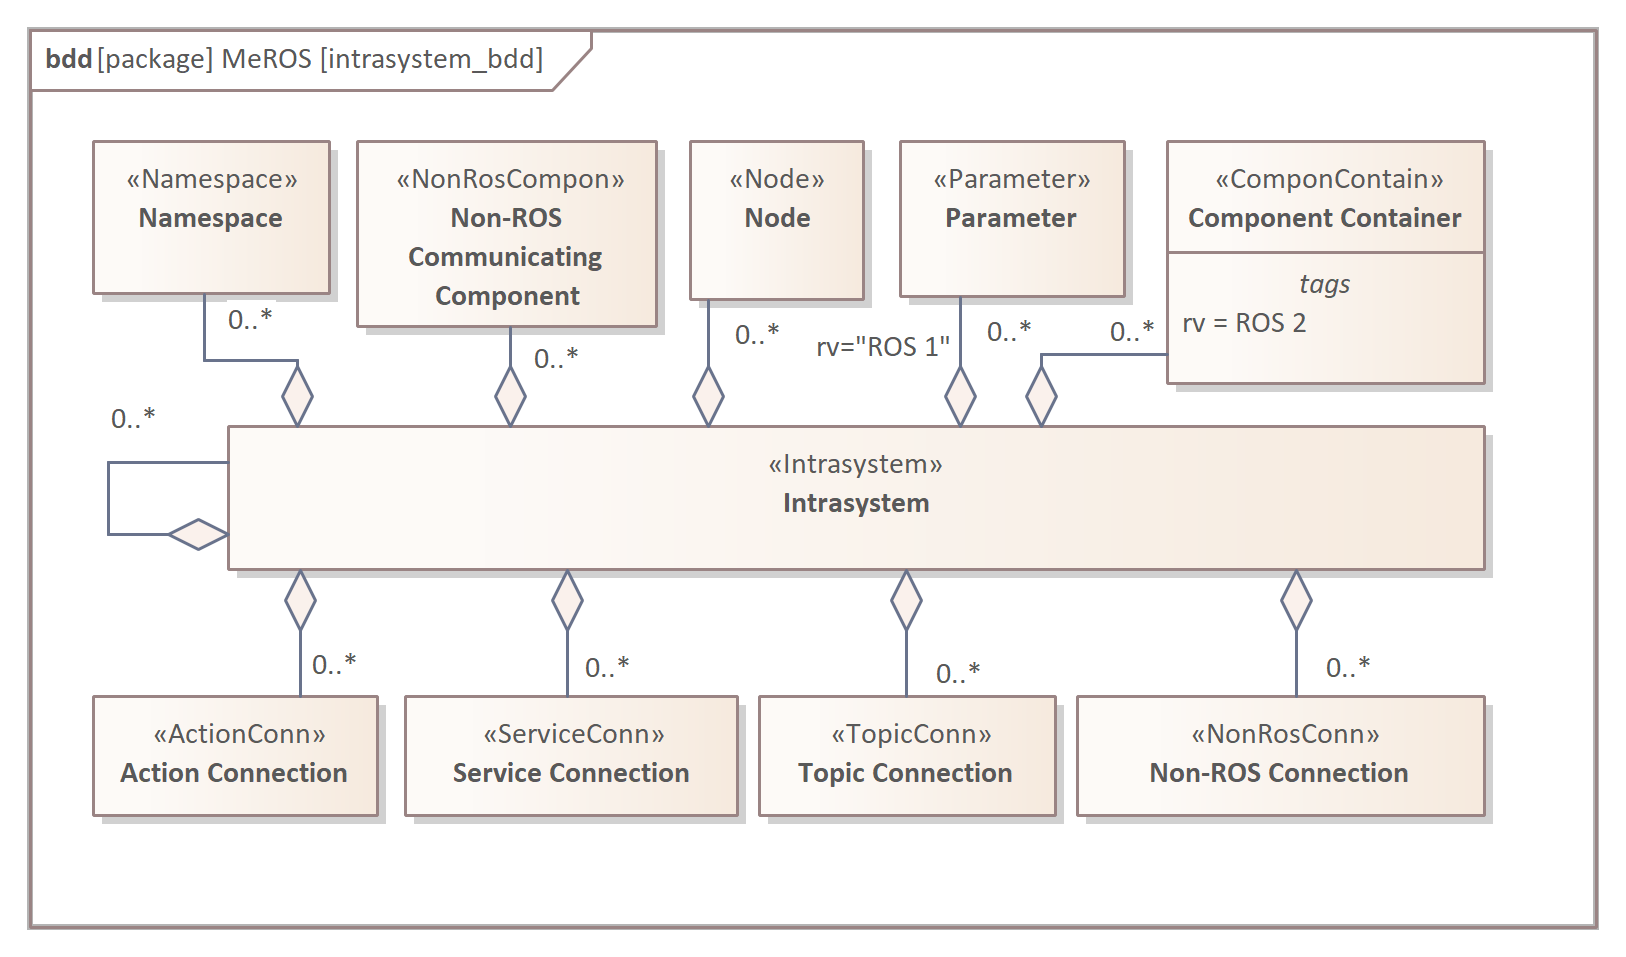
\includegraphics[scale=1.0]{img/meros_pkg/intrasystem_bdd.png}}
		\end{center}
		\caption{Intrasystem compositions -- bdd.} 
		\label{fig:intrasystem_bdd}
	\end{figure} 
	 
  	The Running System (Fig.~\ref{fig:running_system_bdd}) is a specialisation of the Intrasystem that can be executed. Hence, two Nodes are needed for ROS~1: rosout and ROS master. 
	It should be noted that although MeROS could be classified as PSM, the initial, general system description with Communications Channels and Intrasystems corresponds to PIM specification. Then, the detailing of these aggregates corresponds to the transition from PIM to PSM. 
	
		
	\begin{figure}[H]
		\centering
		\begin{center}
			{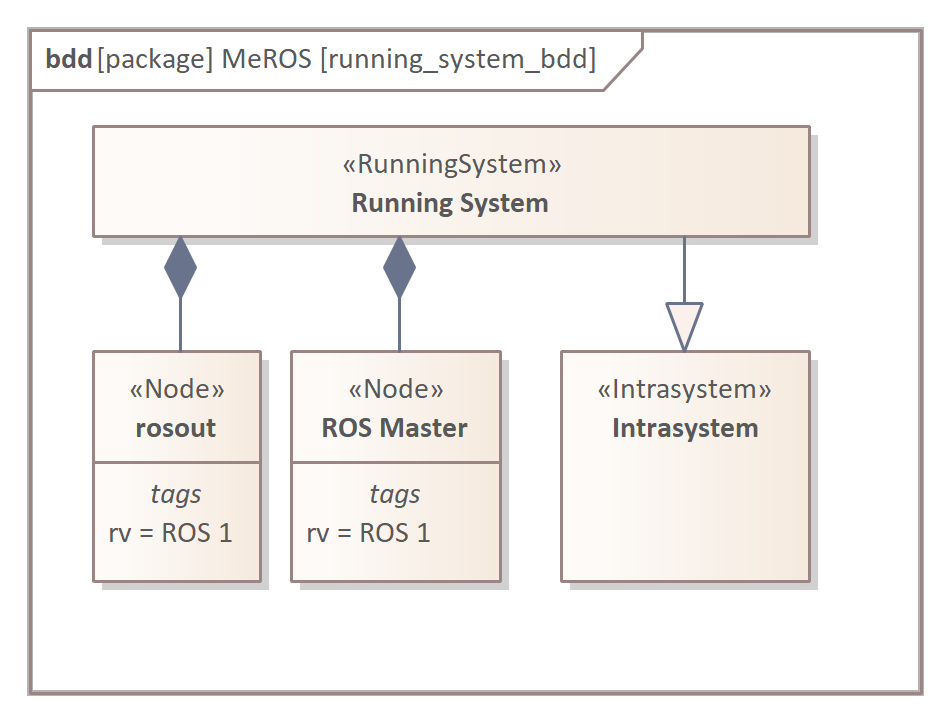
\includegraphics[scale=1.1]{img/meros_pkg/running_system_bdd.png}}
		\end{center}
		\caption{Running System compositions -- bdd.} 
		\label{fig:running_system_bdd}
	\end{figure}
		
	The way Communicating Components use various types of connections is presented in Fig.~\ref{fig:running_system_communication_bdd}. Both ROS and Non-ROS Communicating Components can communicate via Non-ROS Connections, but only ROS Communicating Components use ROS Connections.


	\begin{figure}[H]
		\centering
		\begin{center}
			{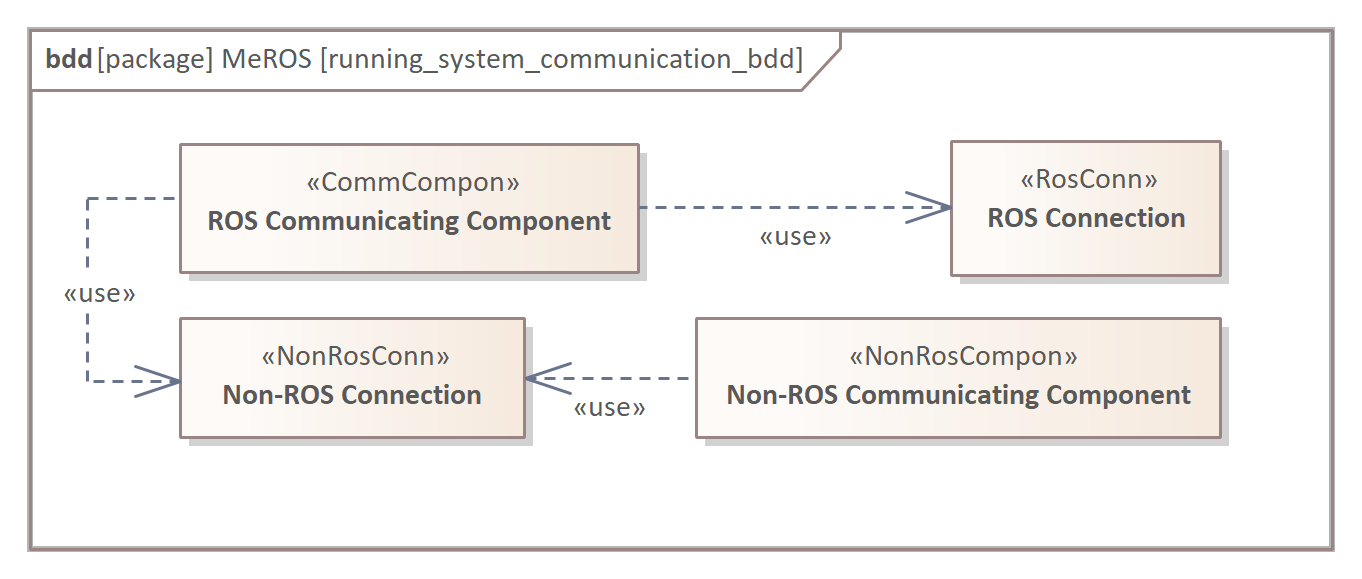
\includegraphics[scale=1.1]{img/meros_pkg/running_system_communication_bdd.png}}
		\end{center}
		\caption{Running System communication -- bdd.} 
		\label{fig:running_system_communication_bdd}
	\end{figure}

	\pagebreak
	
	The Namespace (Fig.~\ref{fig:namespace_bdd}) aggregates elements of the Intrasystem, but only ROS related. In opposition to the Intrasystem, the Namespace does not specialise Communicating Component. Hence, it can not act as Communicating Component.
	
	
	\begin{figure}[H]
		\centering
		\begin{center}
			{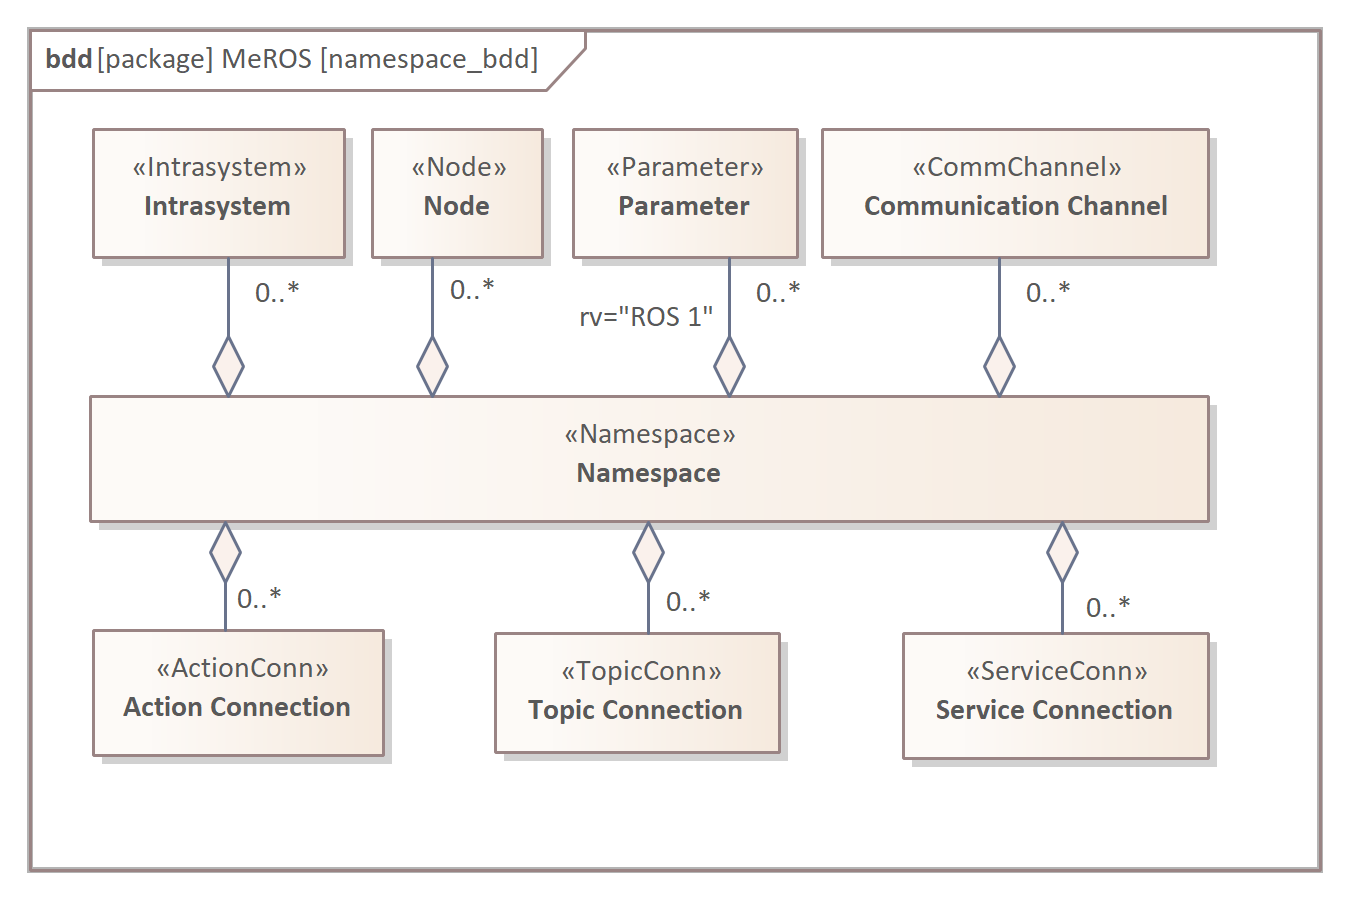
\includegraphics[scale=1.0]{img/meros_pkg/namespace_bdd.png}}
		\end{center}
		\caption{Namespace composition -- bdd.} 
		\label{fig:namespace_bdd}
	\end{figure}
	
	
	The Package (Fig.~\ref{fig:ros_package_bdd}) composes the files related to general ROS concepts such as Node source codes, communication structures definitions, etc. It should be noted that in case of Actions, specific communication structures definitions are stored in Action Data Structures. The Misc <<block>> relates to other ROS and Non-ROS files, e.g., roslaunch configuration, obligatory package.xml, CMakeLists.txt. The Metapackage is introduced for conformity with the latest ROS~1 releases [R7] as well as ROS~2. 
	
	
	\begin{figure}[H]
		\centering
		\begin{center}
			{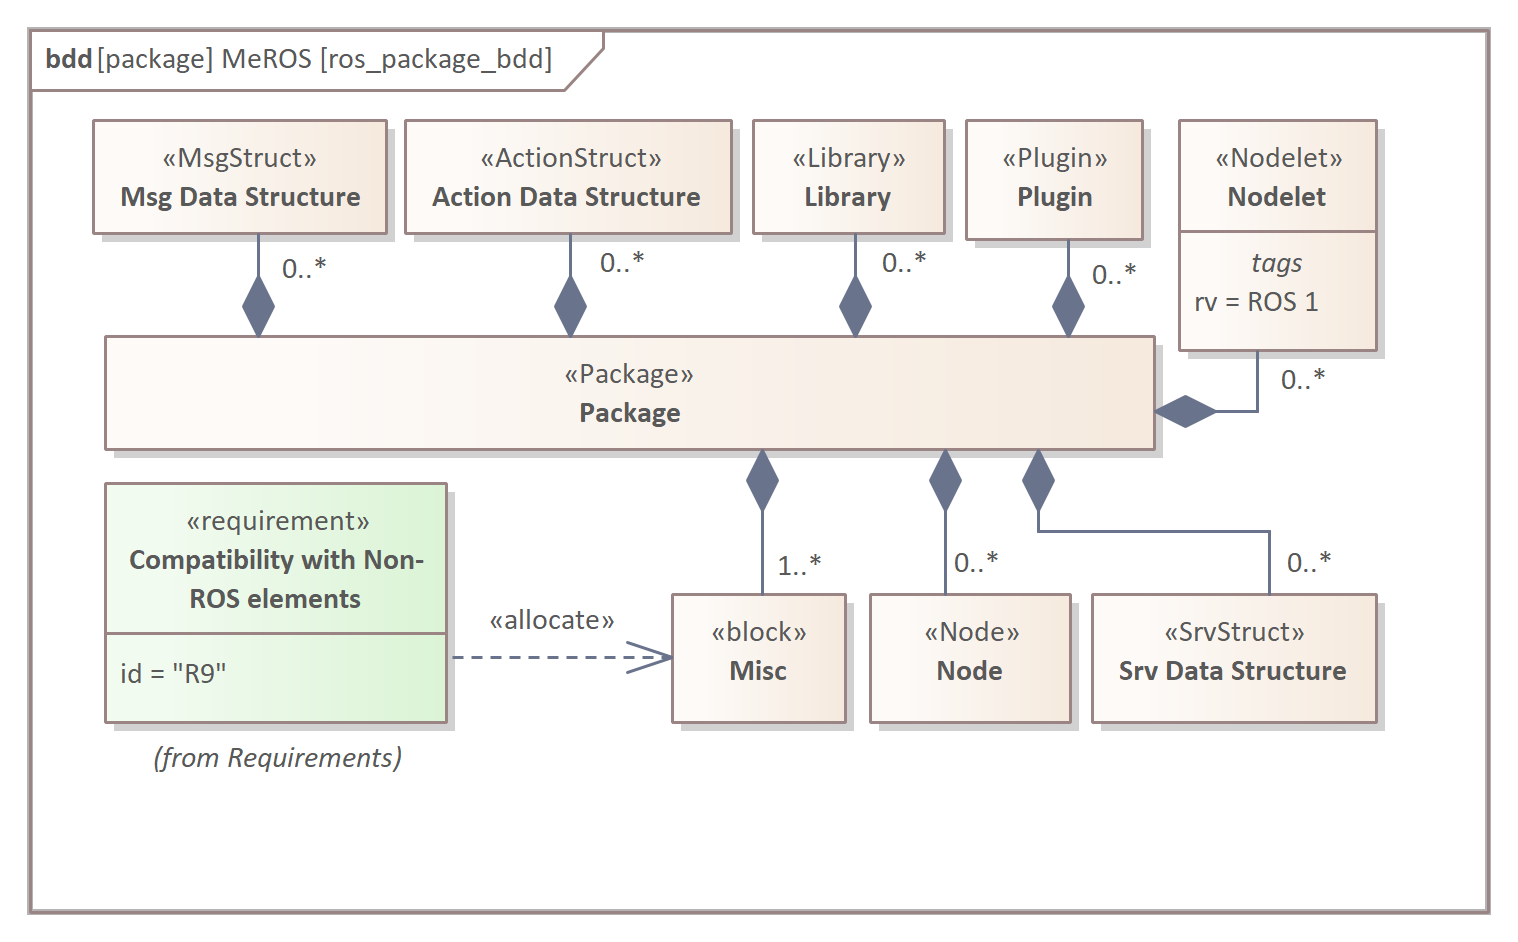
\includegraphics[scale=1.0]{img/meros_pkg/ros_package_bdd.png}}
		\end{center}
		\caption{ROS Package composition -- bdd.} 
		\label{fig:ros_package_bdd}
	\end{figure}
		
	The Workspace (Fig.~\ref{fig:ros_workspace_bdd}) contains of Packages that compose the files related to general ROS concepts such as Node source codes, communication structures definitions, etc. As Workspace has a specific file-system nature, Group of Packages were introduced as a more general component. The Repository plays a similar role to the Workspace, but reflects the place where sources are stored.
	

	\begin{figure}[H]
		\centering
		\begin{center}
			{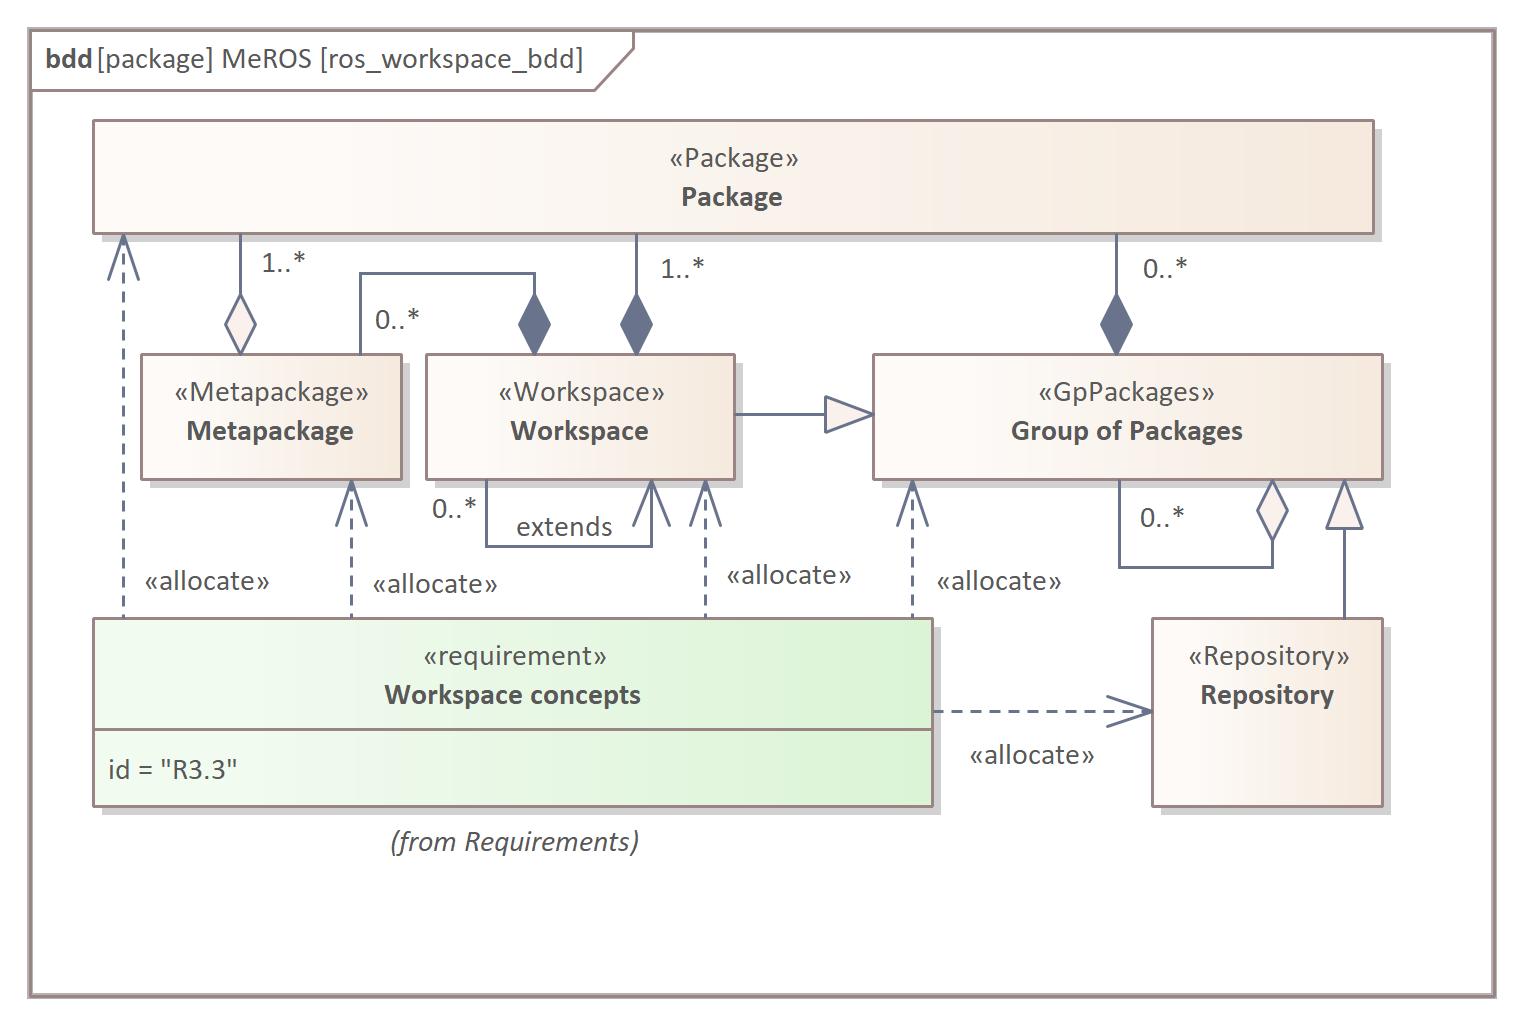
\includegraphics[scale=1]{img/meros_pkg/ros_workspace_bdd.png}}
		\end{center}
		\caption{ROS Workspace composition -- bdd.} 
		\label{fig:ros_workspace_bdd}
	\end{figure}
	

		

	
	
	
\subsection{Communication}
\label{sec:metamodel-communication}
	
	This section depicts the behavioural and structural aspects of communication in the system. The previous section considers block definition diagrams (bdd). In the following part, the internal block diagrams (ibd) and behavioural diagrams are discussed. The goal is to present three modes of communication: Topic [R4.1] (sec.~\ref{sec:metamodel-topic}), Service [R4.2] (sec.~\ref{sec:metamodel-service}) and Action [R4.3] (sec.~\ref{sec:metamodel-action}). It should be noted that the concept of presentation of communication with and without a dedicated communication component is illustrated on communication with Topics but can also be applied to Services, Actions and Communication Channels.
	
		\pagebreak 
	\subsubsection{Topic}
	\label{sec:metamodel-topic}
		
	Fig.~\ref{fig:topic_communication_with_dedicated_component_ibd} presents the ibd diagram of publishers' and subscribers' communication via topics. This diagram uses a dedicated communication component for each Topic [R4.1.1]. There are no general limits to the number of publishers, subscribers and Topics they communicate with. 
	

	\begin{figure}[H]
		\centering
		\begin{center}
			{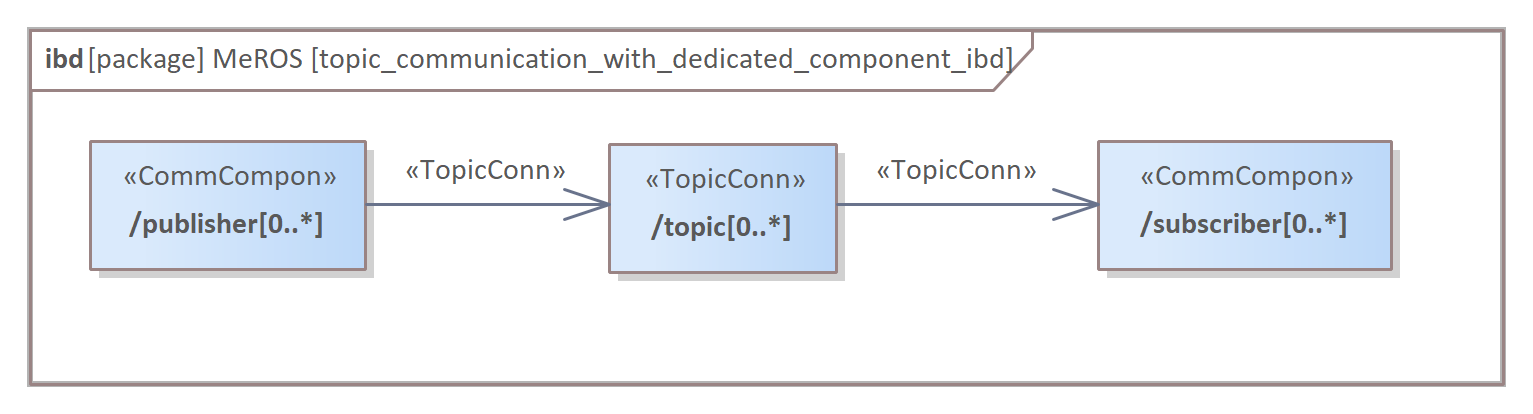
\includegraphics[scale=1.0]{img/meros_pkg/topic_communication_with_dedicated_component_ibd.png}}
		\end{center}
		\caption{Topics with dedicated communication components -- all components -- ibd.} 
		\label{fig:topic_communication_with_dedicated_component_ibd}
	\end{figure}

	Thanks to a dedicated component to represent communication, the diagram in Fig.~\ref{fig:topic_communication_with_dedicated_component_ibd} can be split into two considering publisher (Fig.~\ref{fig:topic_split_publisher_ibd}) and subscriber (Fig.~\ref{fig:topic_split_subscriber_ibd}) separately, without losing information. It is especially useful when system fragments are presented after its decomposition that subdivides communication channels.
	

	\begin{figure}[H]
		\centering
		\begin{center}
			{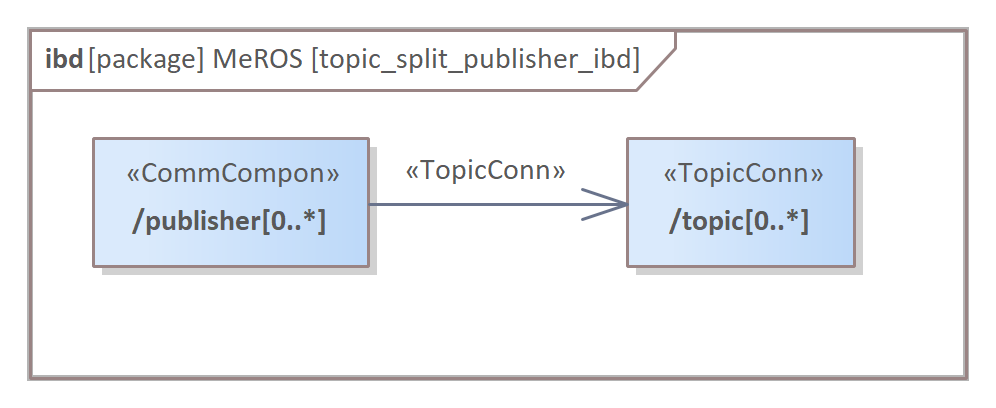
\includegraphics[scale=1.0]{img/meros_pkg/topic_split_publisher_ibd.png}}
		\end{center}
		\caption{Topics with dedicated communication components -- publisher -- ibd.} 
		\label{fig:topic_split_publisher_ibd}
	\end{figure}


	\begin{figure}[H]
		\centering
		\begin{center}
			{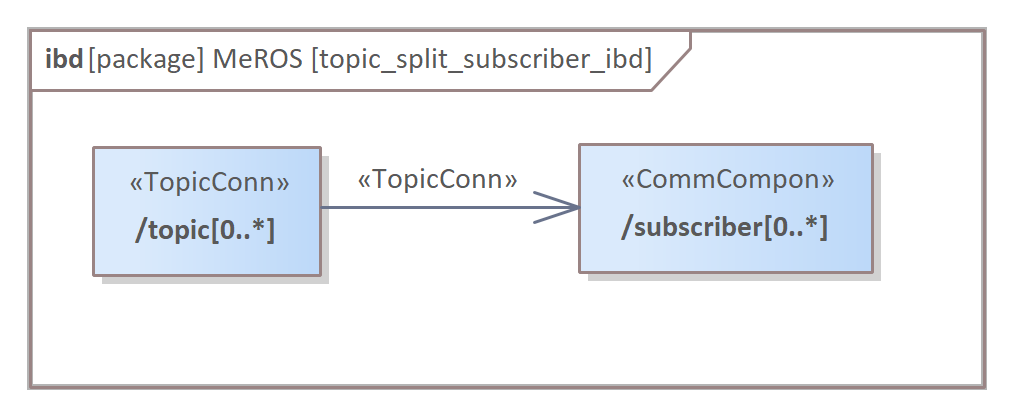
\includegraphics[scale=1.0]{img/meros_pkg/topic_split_subscriber_ibd.png}}
		\end{center}
		\caption{Topics with dedicated communication components -- subscriber -- ibd.} 
		\label{fig:topic_split_subscriber_ibd}
	\end{figure}
	
	
	\pagebreak
	
	Fig. \ref{fig:topic_communication_with_dedicated_component_sd} depicts the corresponding sequence diagram. Publishers send a message through Topics to the subscribers. The incoming message cause the subscriber to execute the callback function. 	Fig.~\ref{fig:topic_communication_without_dedicated_component_ibd} and Fig.~\ref{fig:topic_communication_without_dedicated_component_sd} present an alternative approach to depict the system communicating via topics. In this case, no dedicated communication components are used [R4.1.2]. 
	
	\begin{figure}[H]
		\centering
		\begin{center}
			{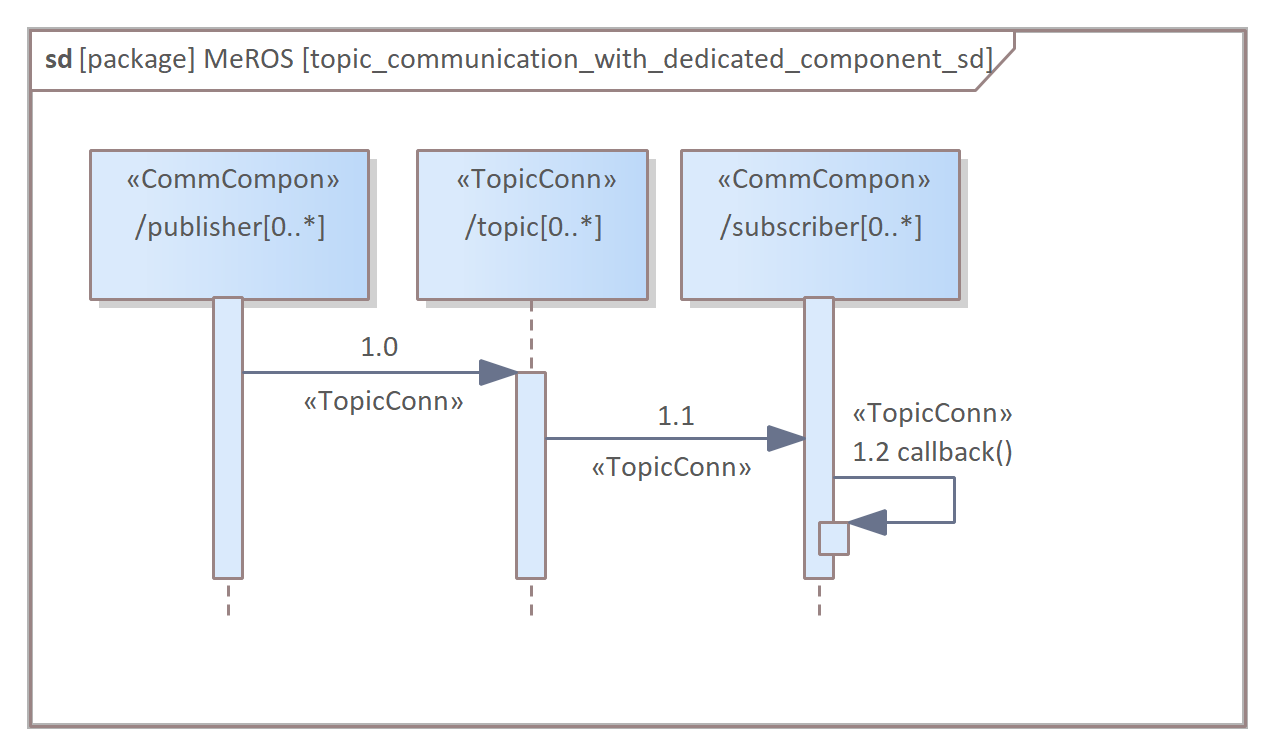
\includegraphics[scale=1.0]{img/meros_pkg/topic_communication_with_dedicated_component_sd.png}}
		\end{center}
		\caption{Topics with dedicated communication components -- sd.} 
		\label{fig:topic_communication_with_dedicated_component_sd}
	\end{figure}
	
	
	\begin{figure}[H]
		\centering
		\begin{center}
			{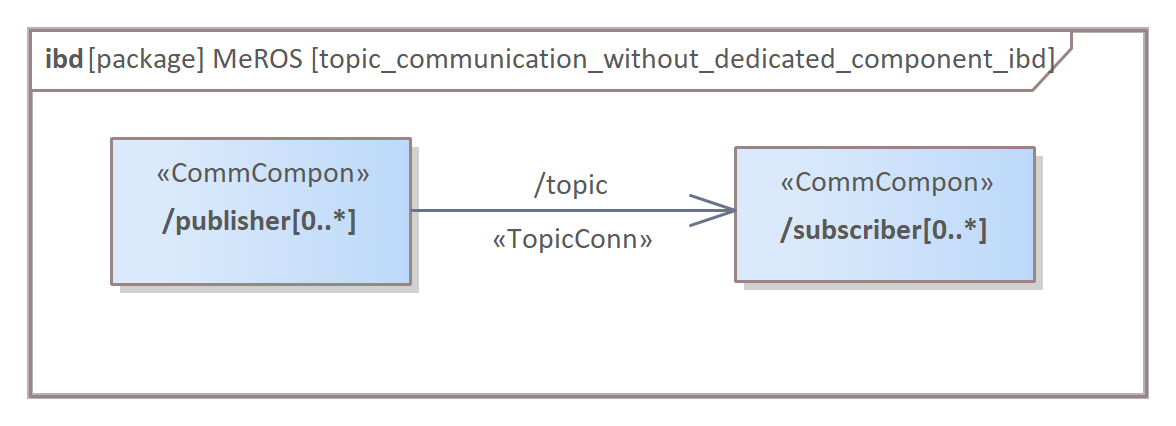
\includegraphics[scale=1.0]{img/meros_pkg/topic_communication_without_dedicated_component_ibd.png}}
		\end{center}
		\caption{Topics without dedicated communication components -- ibd.} 
		\label{fig:topic_communication_without_dedicated_component_ibd}
	\end{figure}
	
	\begin{figure}[H]
		\centering
		\begin{center}
			{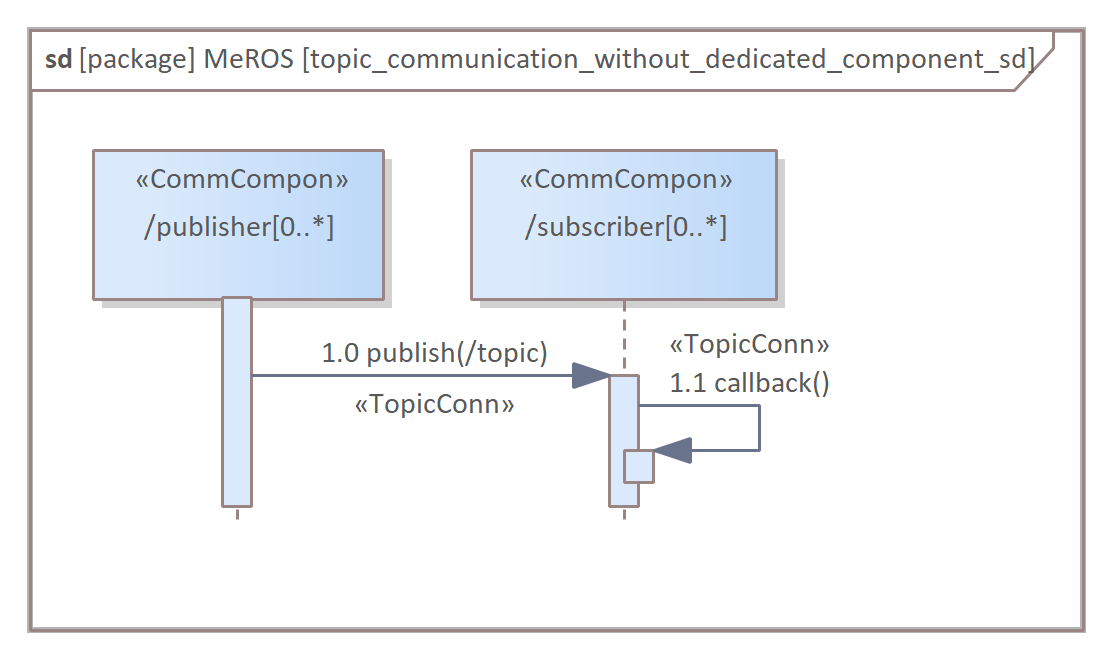
\includegraphics[scale=1.0]{img/meros_pkg/topic_communication_without_dedicated_component_sd.png}}
		\end{center}
		\caption{Topics without dedicated communication components -- sd.} 
		\label{fig:topic_communication_without_dedicated_component_sd}
	\end{figure}
	
\subsubsection{Service}
\label{sec:metamodel-service}
	
	For each ROS Service, there is at most one server and a~number of clients (Fig.~\ref{fig:service_communication_ibd} and Fig.~\ref{fig:service_communication_sd}). Service-type communication is bidirectional and realises RPC (remote procedure call).
	

	\begin{figure}[H]
		\centering
		\begin{center}
			{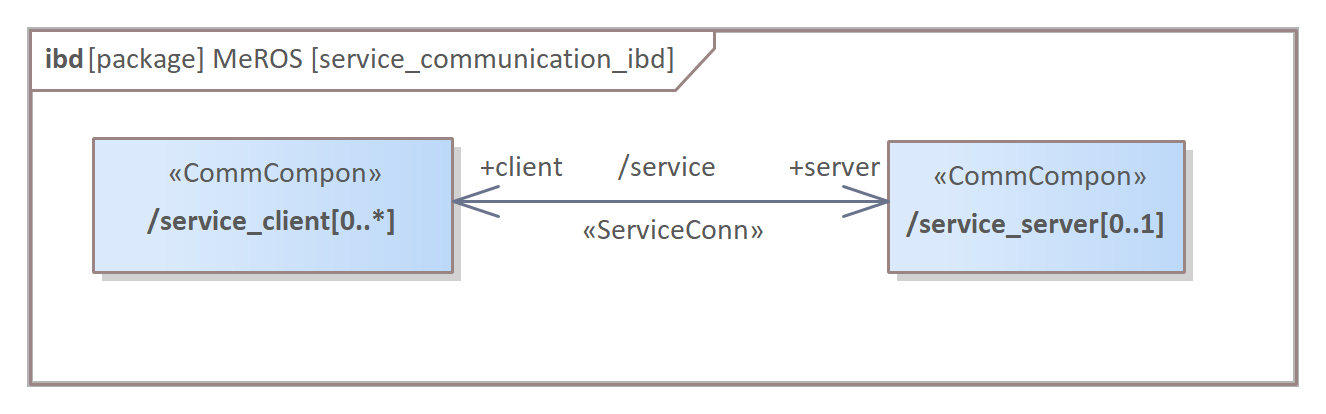
\includegraphics[scale=1.0]{img/meros_pkg/service_communication_ibd.png}}
		\end{center}
		\caption{Service-based communication -- ibd.} 
		\label{fig:service_communication_ibd}
	\end{figure}
	

	\begin{figure}[H]
		\centering
		\begin{center}
			{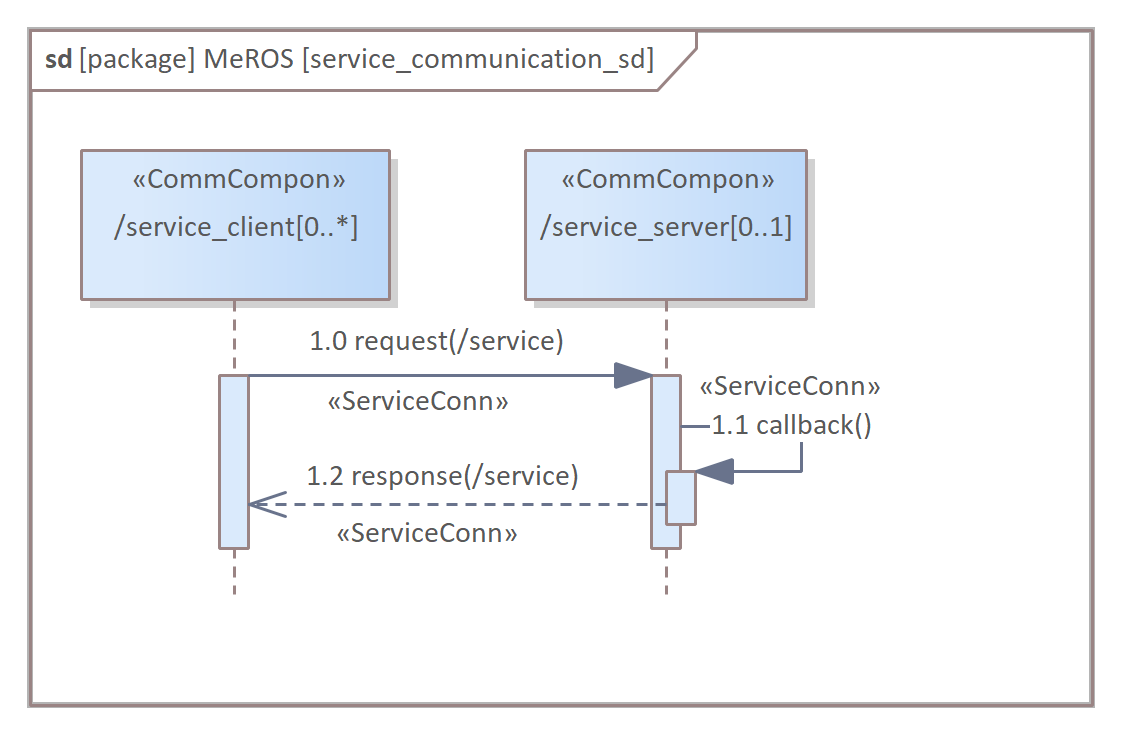
\includegraphics[scale=1.0]{img/meros_pkg/service_communication_sd.png}}
		\end{center}
		\caption{Service-based communication -- sd.} 
		\label{fig:service_communication_sd}
	\end{figure}
	
	
\subsubsection{Action}
\label{sec:metamodel-action}
	
	ROS Action communication's general, simplified structure (Fig.~\ref{fig:action_communication_compact_ibd}) is analogous to ROS Service. These type of presentation is universal for ROS~1 and ROS~2.
	

	\begin{figure}[H]
		\centering
		\begin{center}
			{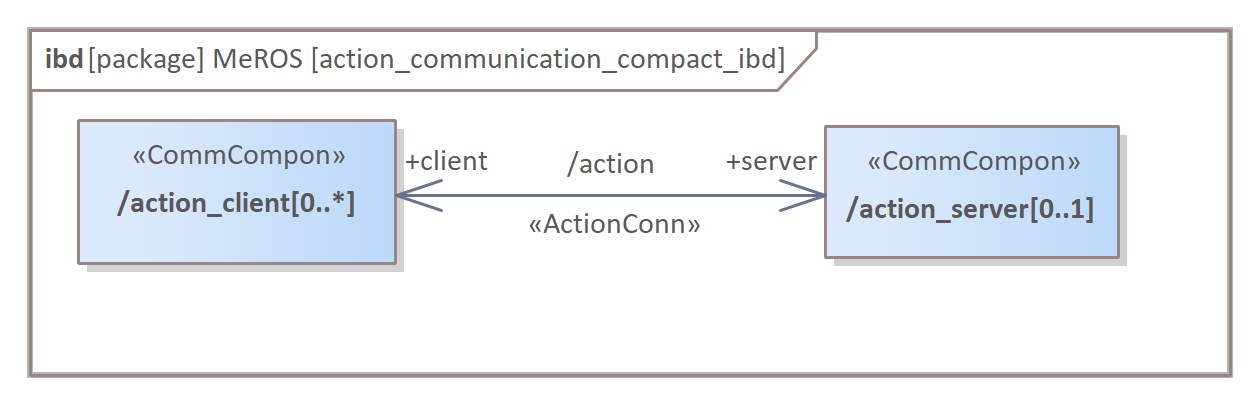
\includegraphics[scale=1.0]{img/meros_pkg/action_communication_compact_ibd.png}}
		\end{center}
		\caption{Action-based communication -- compact representation -- ibd.} 
		% https://docs.ros.org/en/foxy/Tutorials/Beginner-CLI-Tools/Understanding-ROS2-Actions/Understanding-ROS2-Actions.html
		\label{fig:action_communication_compact_ibd}
	\end{figure}
		
	\pagebreak
	
	 An Action (Fig.~\ref{fig:action_communication_detailed_ibd}) is based on several Topics in ROS~1, while on Topics and Services in ROS~2.
	

	\begin{figure}[H]
		\centering
		\begin{center}
			{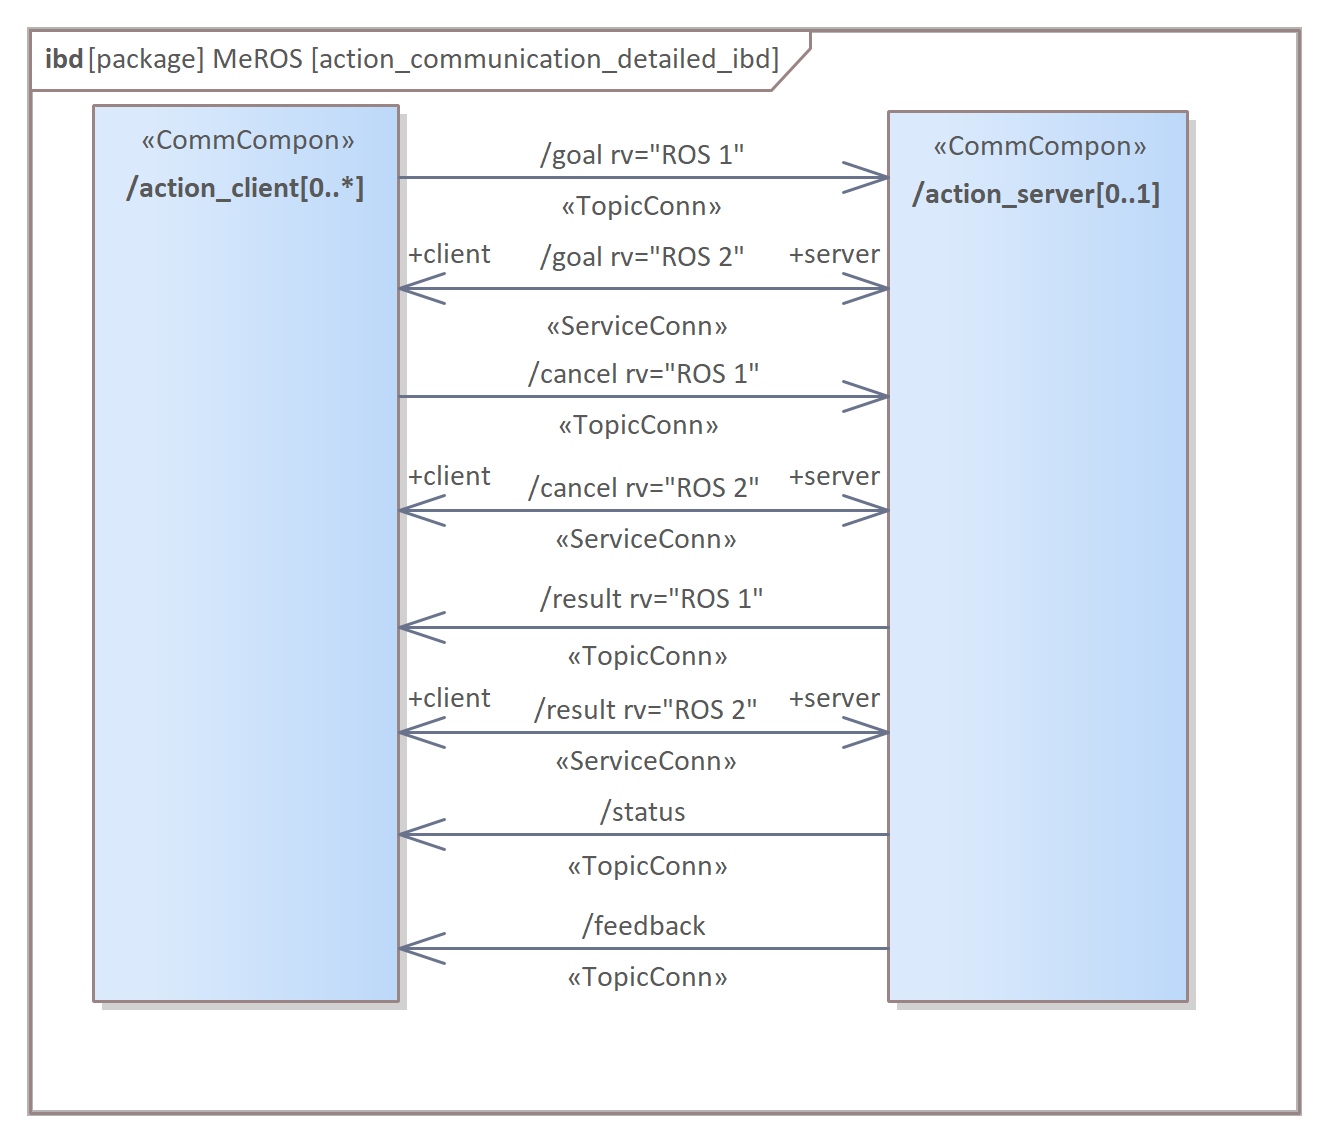
\includegraphics[scale=1.0]{img/meros_pkg/action_communication_detailed_ibd.png}}
		\end{center}
		\caption{Action-based communication -- detailed -- ibd.} 
		% https://design.ros2.org/articles/actions.html
		\label{fig:action_communication_detailed_ibd}
	\end{figure}
	
	In practice, to present an action-related communication compactly on sd diagram (Fig.~\ref{fig:action_communication_compact_sd}) particular Topics and Services can be generalised as a~request (for /goal and /cancel) and a~response (for /status, /feedback and /result). It should be noted that this diagram presents the Action communication sequence in a simplified way.
	
	\begin{figure}[H]
		\centering
		\begin{center}
			{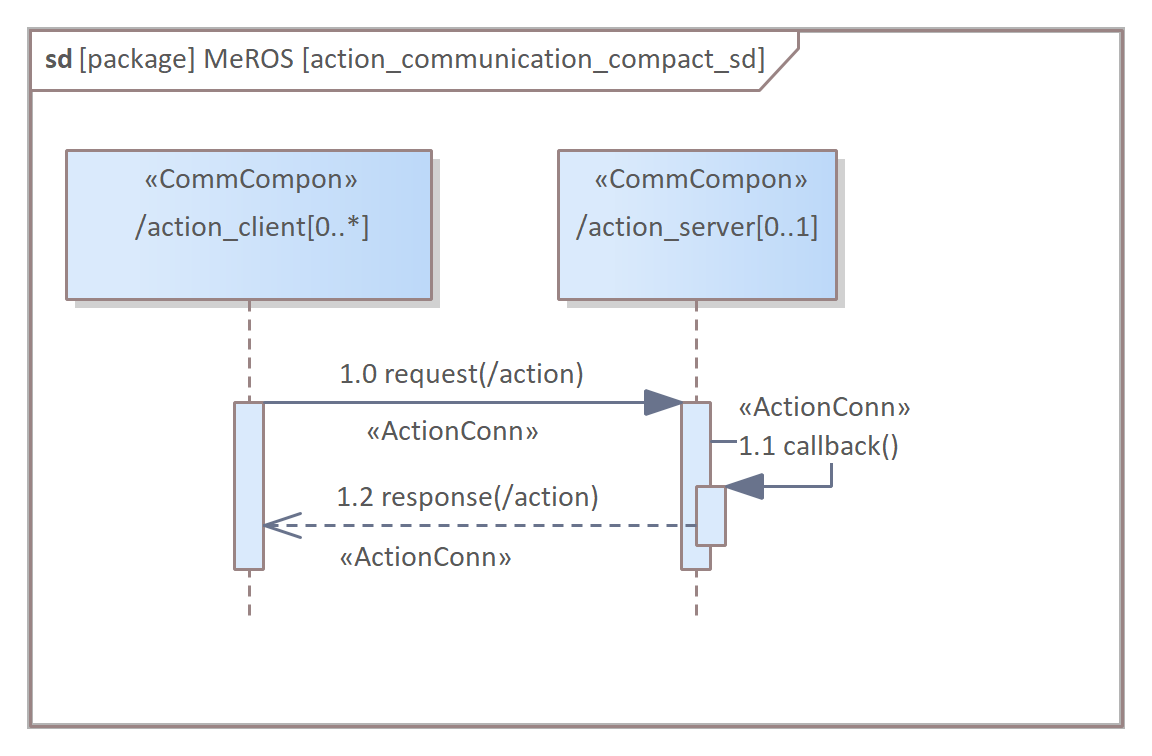
\includegraphics[scale=1.0]{img/meros_pkg/action_communication_compact_sd.png}}
		\end{center}
		\caption{Action-based communication sequence -- compact presentation -- sd.} 
		\label{fig:action_communication_compact_sd}
	\end{figure}

\pagebreak

	The detailed behaviour of the Action server and Action client in ROS~1 is specified by state machines \footnote{\url{http://wiki.ros.org/actionlib/DetailedDescription}}. ROS~2 Action server and Action client behaviour is analogous. Here, these two state machines are depicted in stm diagrams. In the description, in addition to the original ROS wiki presentation, the Topics are directly mentioned both in transitions and states actions.
	 Fig.~\ref{fig:ros1_action_server_stm} depicts the ROS~1 Action server state machine.
	  Its transitions depend on the new messages sent by the Action client or internal predicates. 
	  
	\begin{figure}[H]
		\centering
		\begin{center}
			{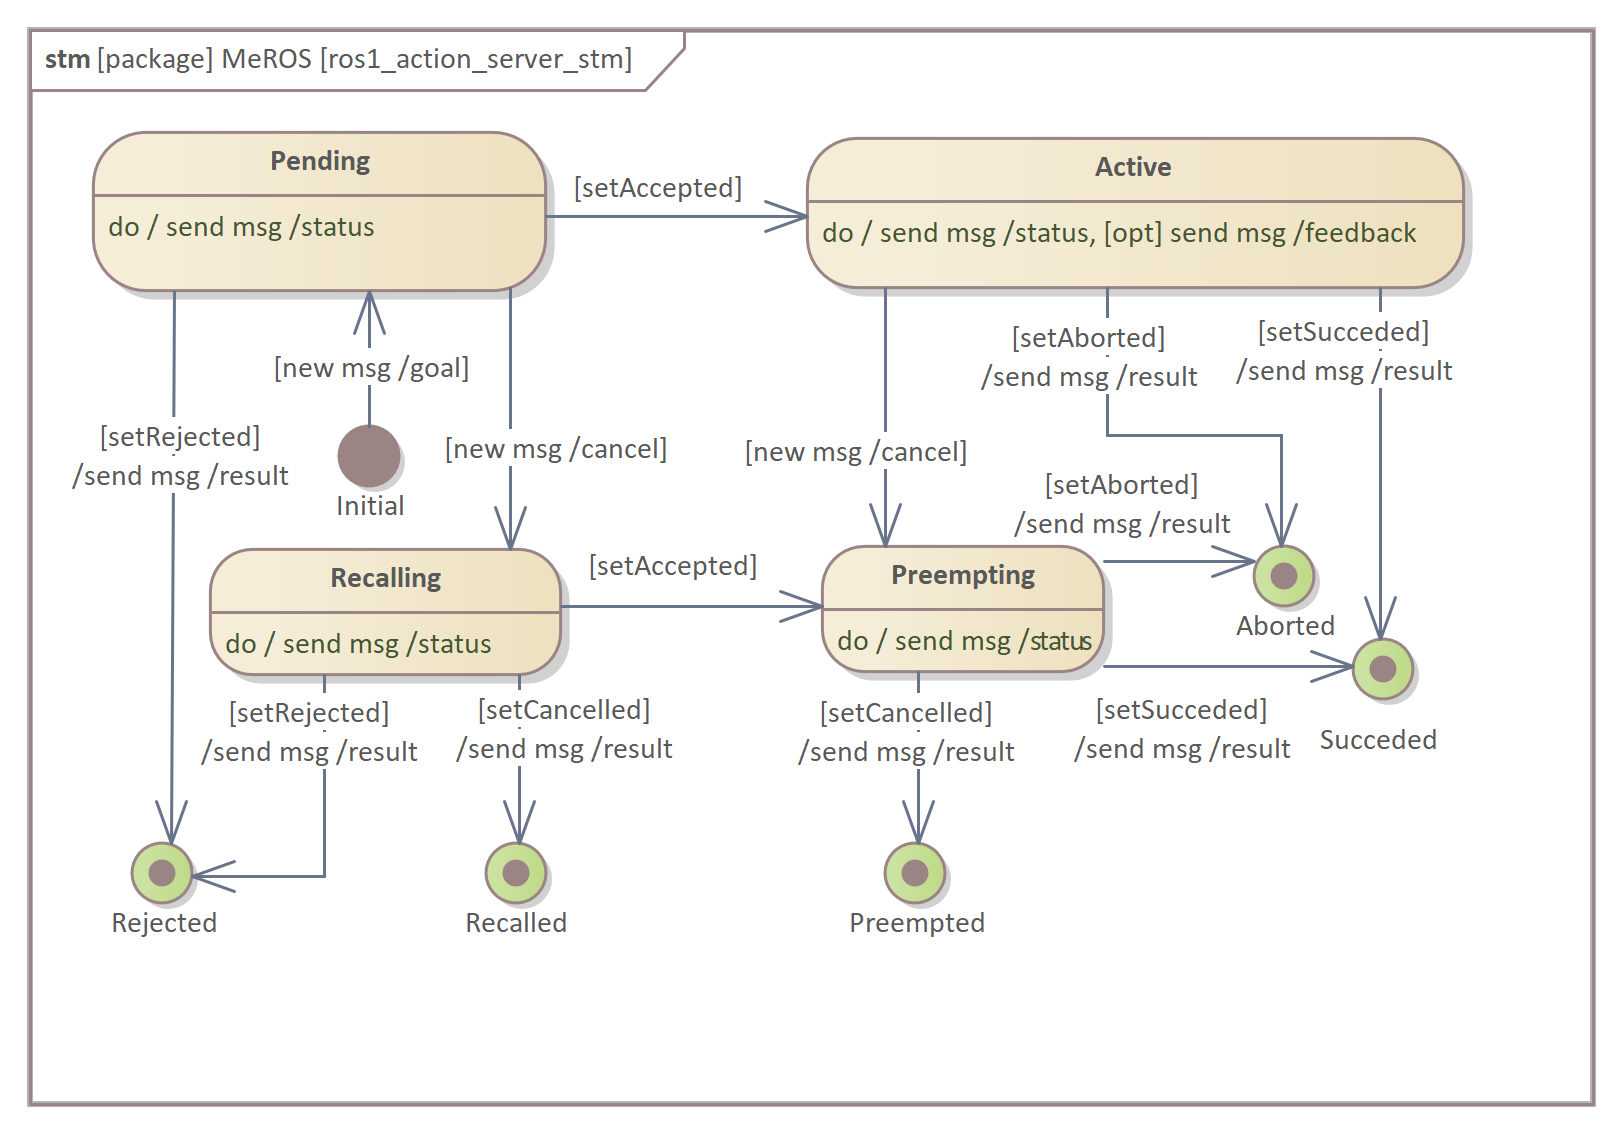
\includegraphics[scale=1.1]{img/meros_pkg/ros1_action_server_stm.png}}
		\end{center}
		\caption{ROS~1 Action server -- stm.} 
		\label{fig:ros1_action_server_stm}
	\end{figure}
	
	\pagebreak
	
	
	The ROS~1 Action client state machine (Fig.~\ref{fig:ros1_action_client_stm}) depends on the server state provided by the Action server in /status Topic and internal predicates. 
		
	\begin{figure}[H]
		\centering
		\begin{center}
			{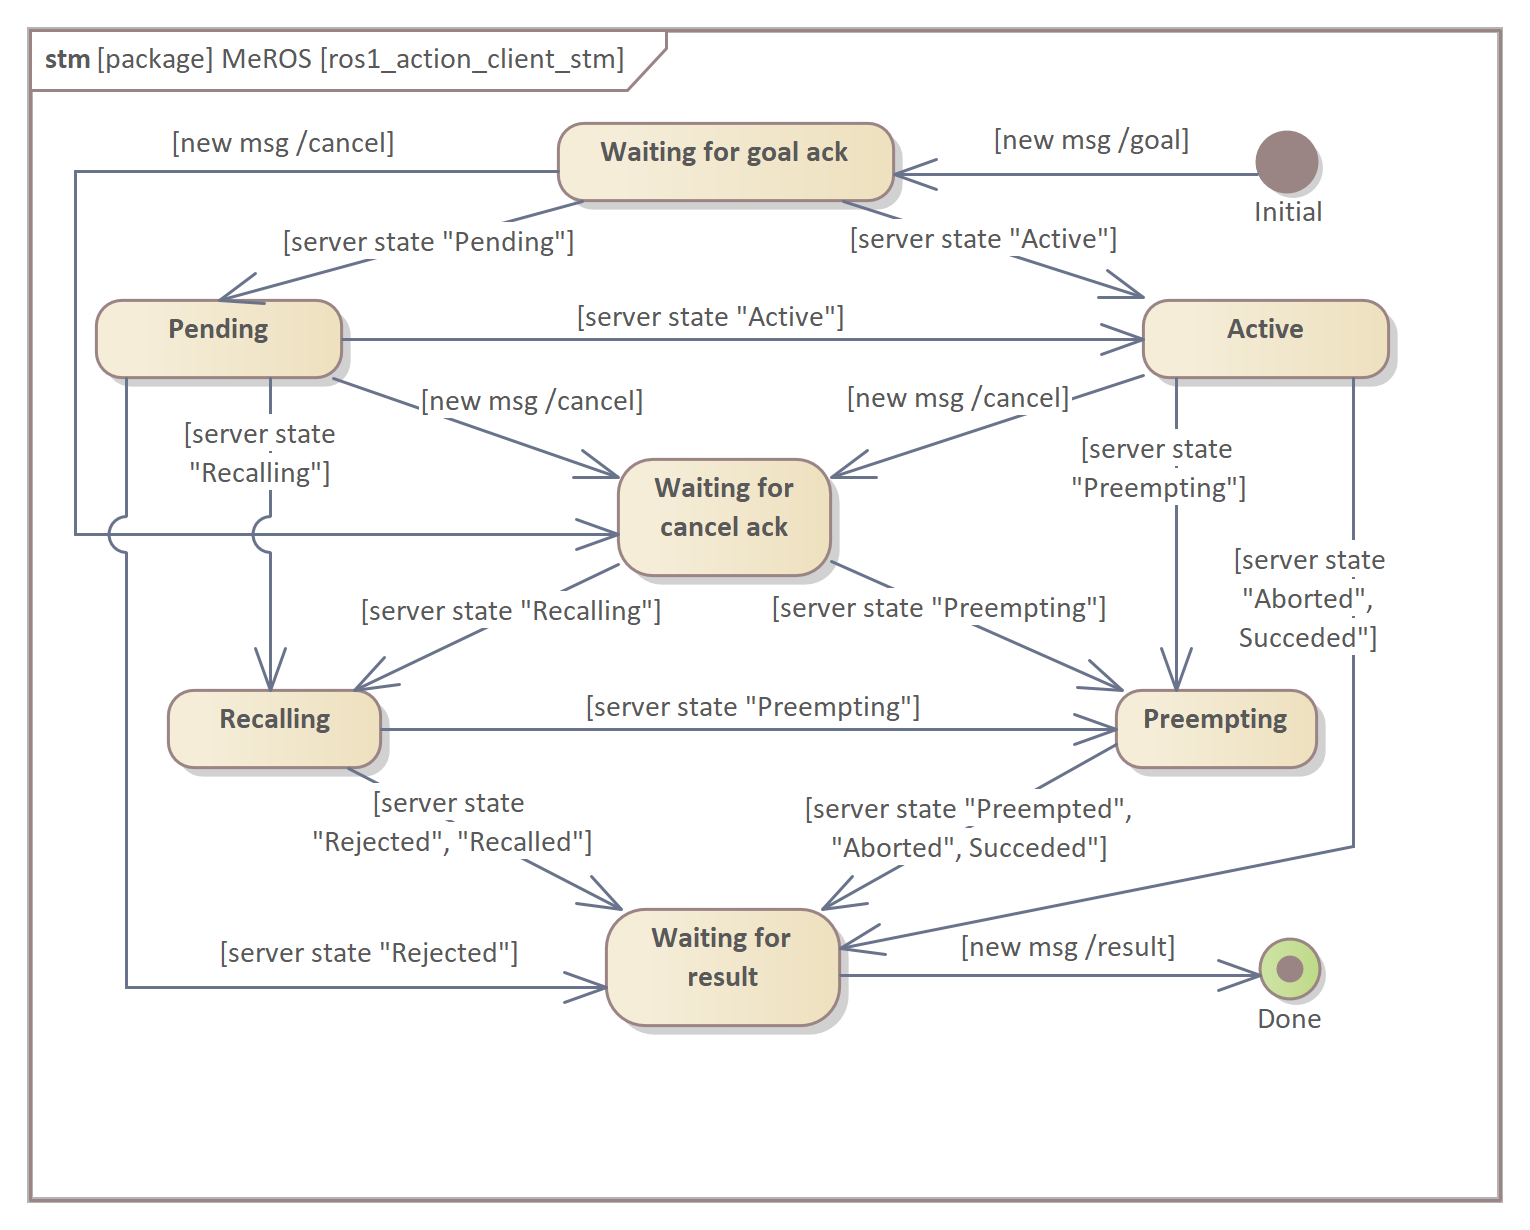
\includegraphics[scale=1.0]{img/meros_pkg/ros1_action_client_stm.png}}
		\end{center}
		\caption{ROS~1 Action client -- stm.}
		\label{fig:ros1_action_client_stm}
	\end{figure}
	
	
\section{MeROS application}
\label{sec:application}
	
	
\subsection{Application hints}
\label{sec:application-hints}

	MeROS metamodel can be employed in various ways in broad context of SE. Although, it is difficult to speak of an indication of the best procedure for its application, it is possible to formulate some practical guidelines for building a particular system model based on MeROS. 

	\begin{itemize}
		\item Before defining a SysML Object, one must define the Block of which it is an instance. It is best to place Block definitions on the bdd diagrams as well. Afterwards, the definition of Objects and the formulation of the other diagrams can follow.
		\item The Object is an instance of the Block, and the Object's classifier corresponds to the Block's name. The Object's name specifies the name of the Block instance. The stereotypes for Block and Object are the same.
		\item The same Blocks and the same Objects should not be duplicated. A Block or Object is defined once and used in different diagrams (in particular, the same Blocks in both the Running System and Workspace diagrams or Objects in the ibd and sd diagrams).
		\item In practice, as long as automatic validation of models formulated in MeROS is not planned, there is no need to formulate a complete model in a SysML project. 
	\end{itemize}
		
	To help develop user projects, the MeROS UML profile and other materials are accessible from MeROS project page\footnote{\url{http://github.com/twiniars/meros}}. 
	
	
\subsection{Exemplary system}
\label{sec:application-example}

	This section presents key aspects of an exemplary system development process incorporating MeROS. The exemplary system was created within the AAL INCARE project to control the Rico assistive robot (modified TIAGo platform with controller based on ROS~1) to execute transportation attendance tasks (Fig.~\ref{fig:herbatka_u_winiara}).
	
	\begin{figure}[H]
		\centering
		\begin{center}
			{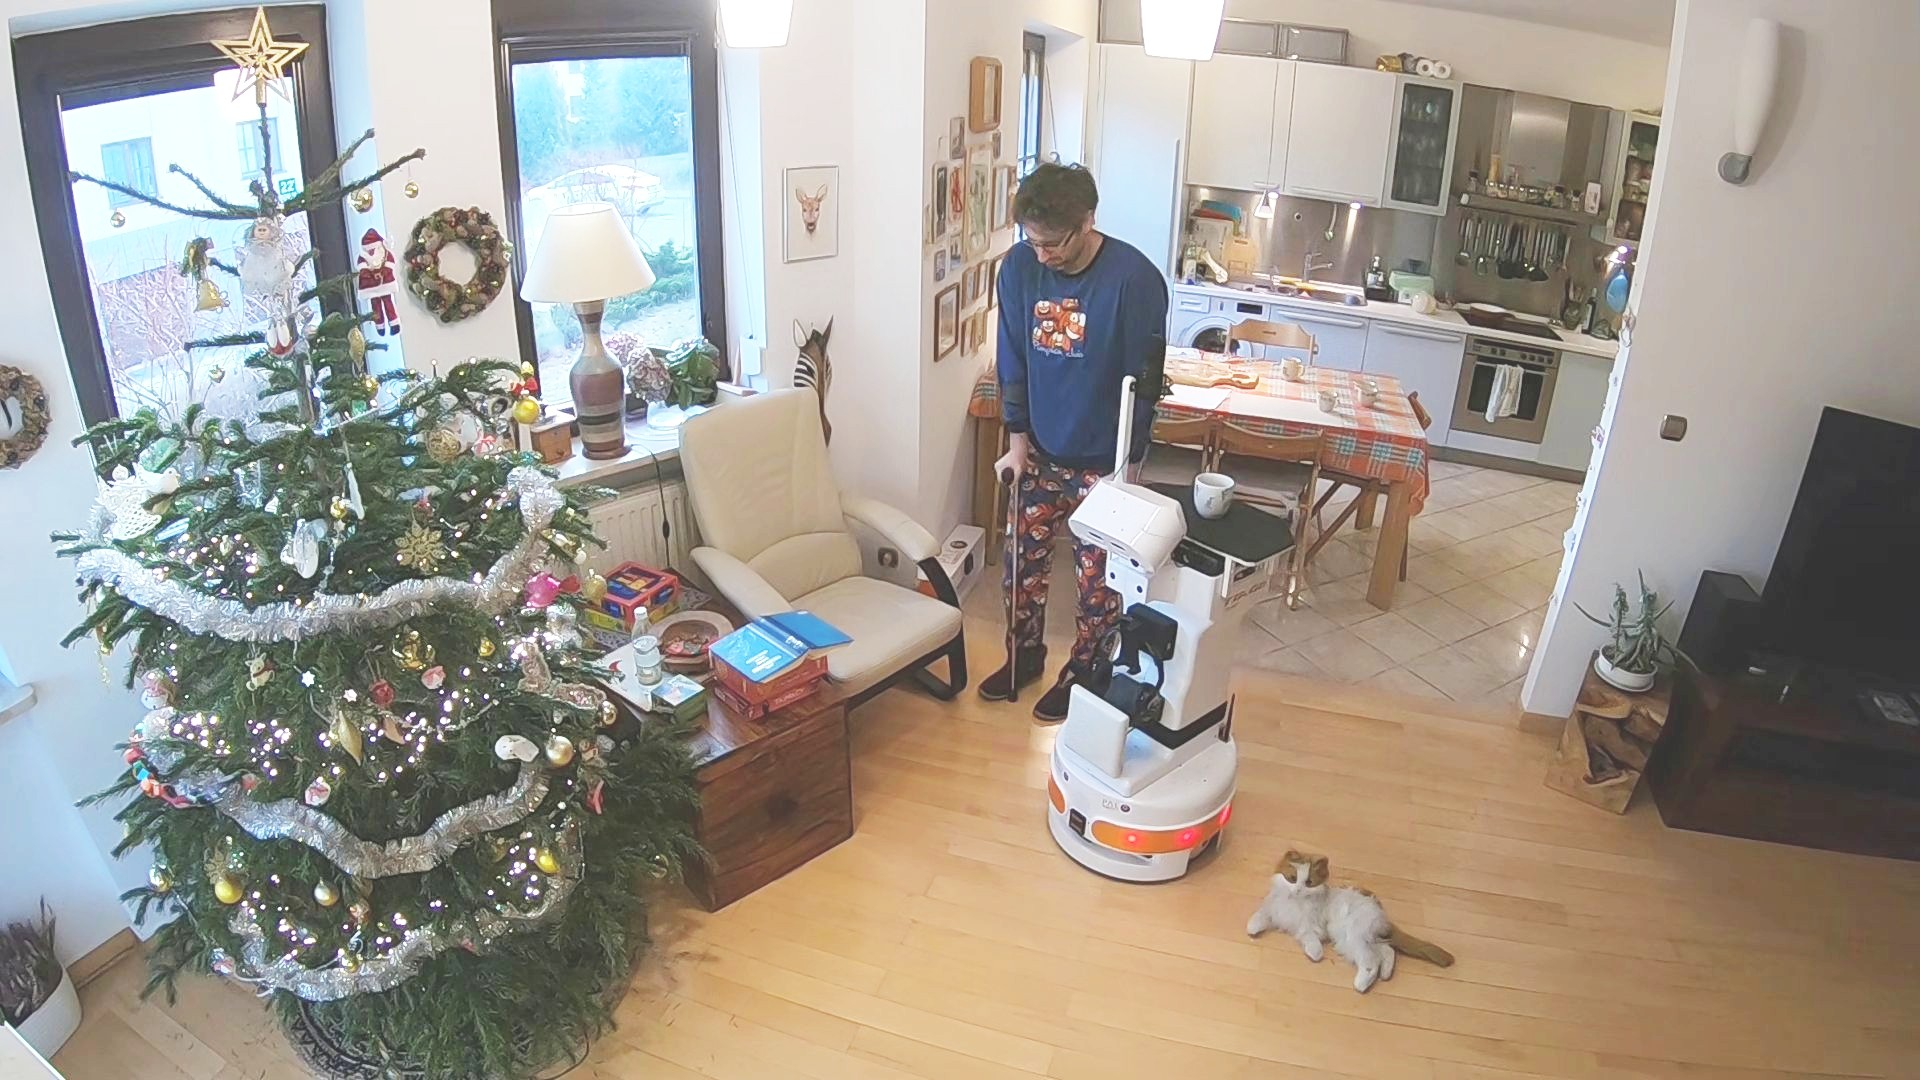
\includegraphics[width=0.9\columnwidth]{img/herbatka_u_winiara.jpg}}
		\end{center}
		\caption{Transportation attendance by Rico robot \url{https://vimeo.com/670252925}} 
		\label{fig:herbatka_u_winiara}
	\end{figure}
	
	
	
	 The purpose of the following description is not to document the entire system but to illustrate, by example, representative aspects of the MeROS application.
	 
	 \pagebreak
	 
	The part of the application scenario is conceptually presented in Fig.~\ref{fig:general_sd}.
	

	\begin{figure}[H] 
		\centering
		\begin{center}
			{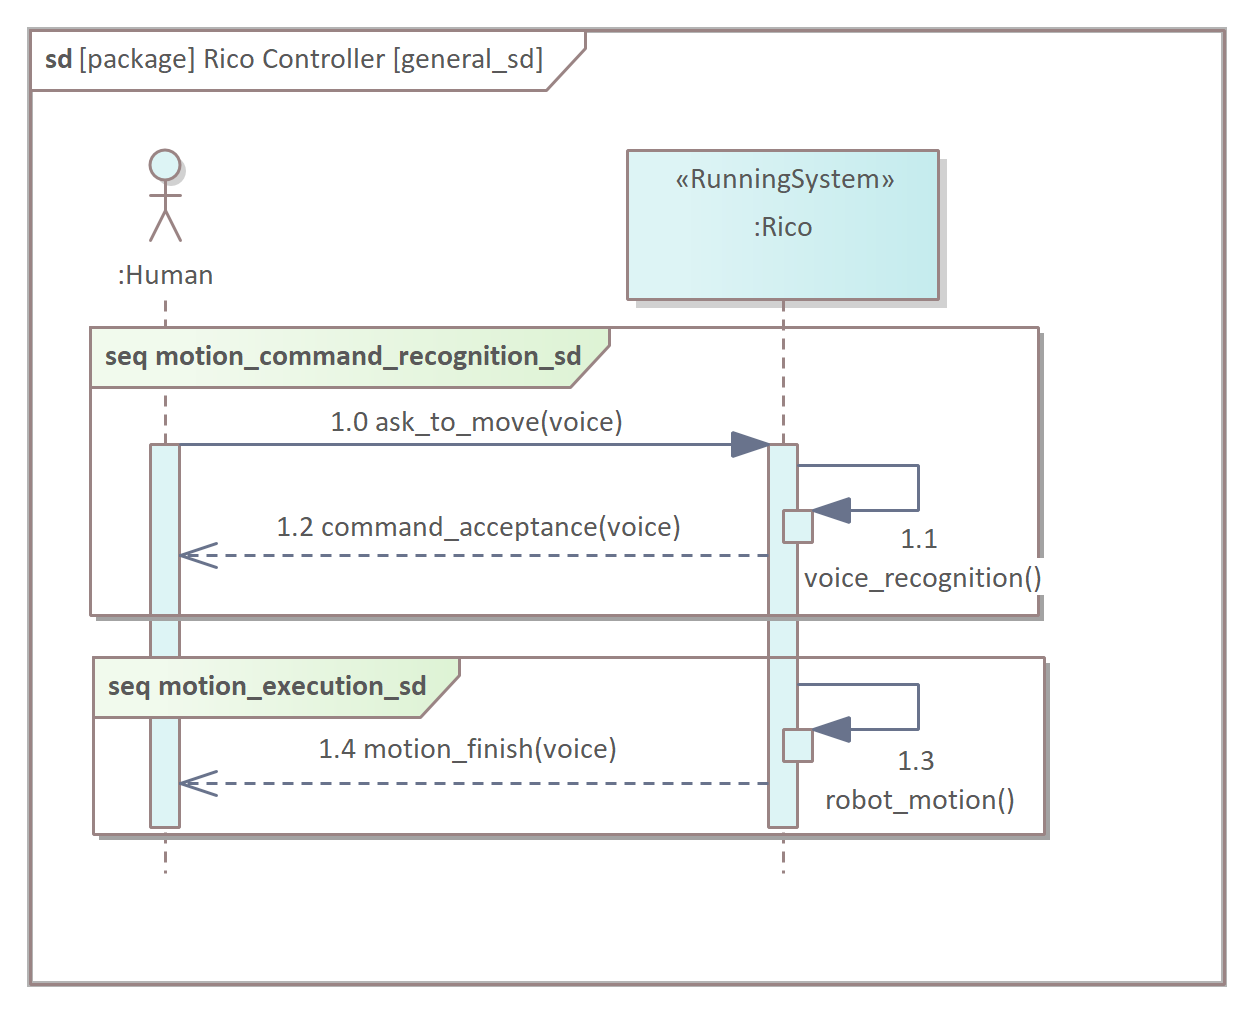
\includegraphics[scale=0.95]{img/rico_pkg/general_sd.png}}
		\end{center}
		\caption{Concept scenario -- sd.} 
		\label{fig:general_sd}
	\end{figure}
	
	Here, the system (<<RunningSystem>> \texttt{:Rico}) and its behaviour are formulated in a~general way. An actor (e.g. an elderly person) asks the robot to move. Then, the system recognises the voice command and vocally confirms the command's acceptance. Finally, the robot executes the motion and vocally informs that the motion is finished.
	In the following part of the description, the <<RunningSystem>> \texttt{:Rico} and sequence diagram frame \texttt{motion execution} from Fig.~\ref{fig:general_sd} are presented in a explicit way.
	The block definition diagram in Fig.~\ref{fig:rico_running_system_bdd} depicts the composition of <<RunningSystem>> \texttt{:Rico}.
	
	\begin{figure}[H]
		\centering
		\begin{center}
			{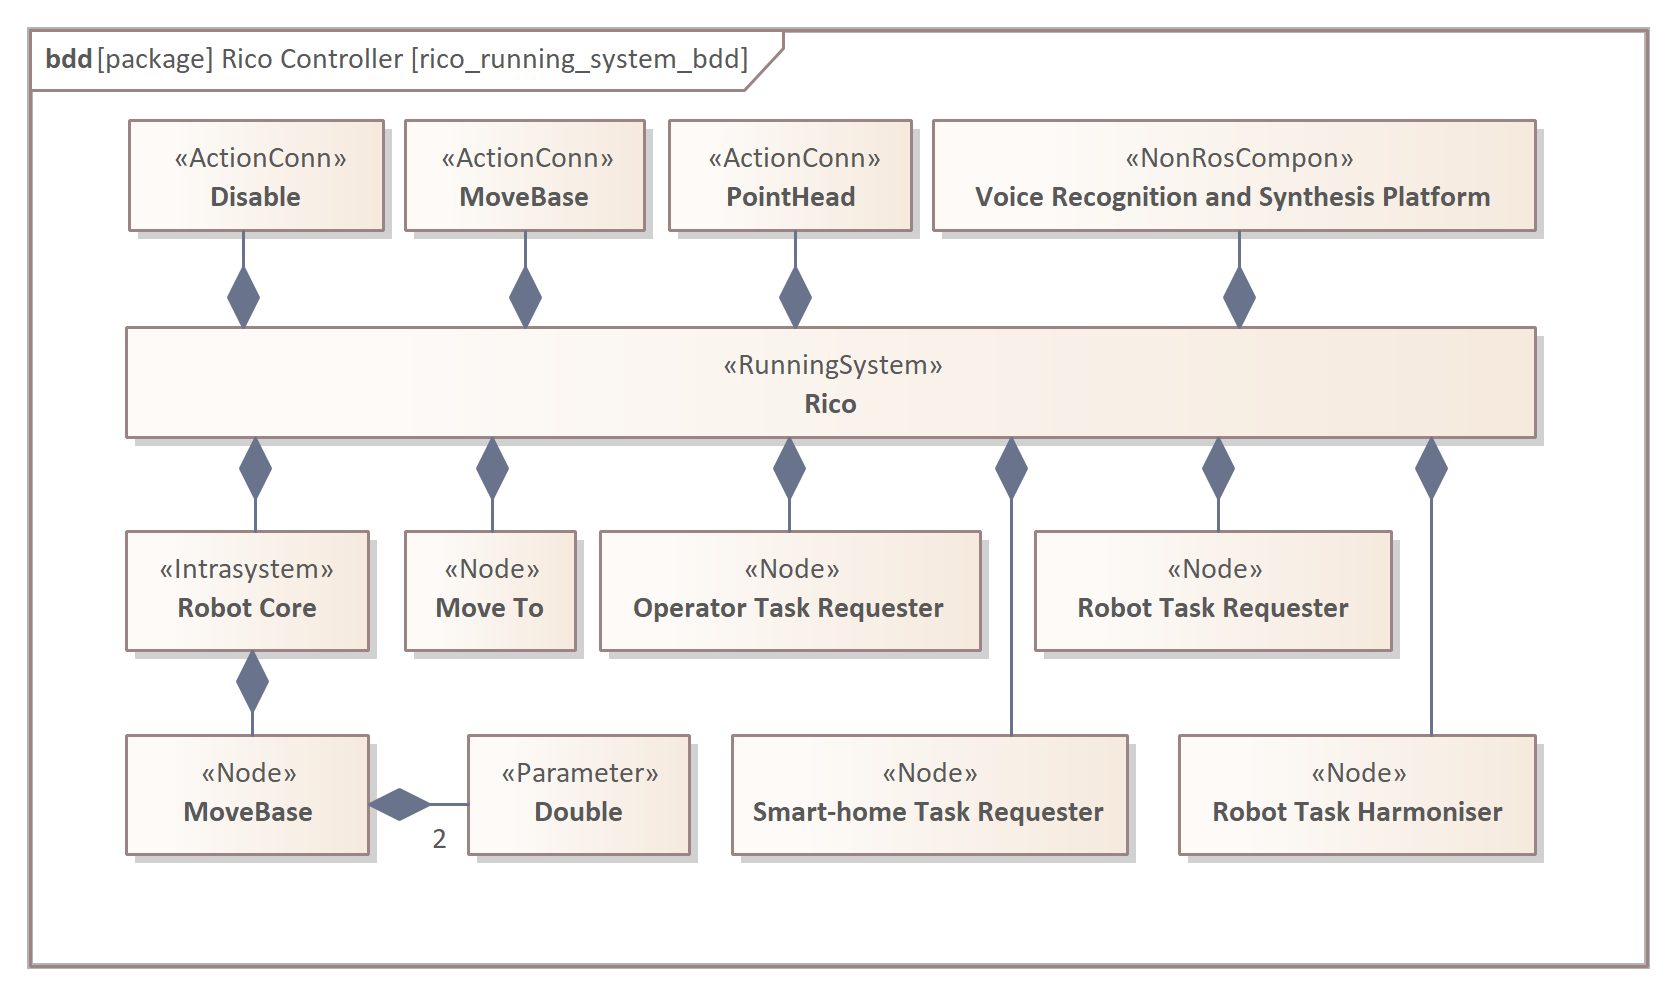
\includegraphics[scale=0.95]{img/rico_pkg/rico_running_system_bdd.png}}
		\end{center}
		\caption{Rico <<RunningSystem>> composition -- bdd.}
		\label{fig:rico_running_system_bdd}
	\end{figure}
	
	The <<RunningSystem>> \texttt{:Rico} structure is depicted in Fig.~\ref{fig:rico_running_system_ibd}. Here, and in the following diagrams, the \texttt{rosout} and \texttt{ROS master} <<Node>>s were omitted to make the diagrams more compact. The specific label is needed for <<CommChannel>>, e.g., <<CommChannel>> \texttt{:Move To to Robot Core}, because this <<CommChannel>> is described later on.
	
	\begin{figure}[H]
		\centering
		\begin{center}
			{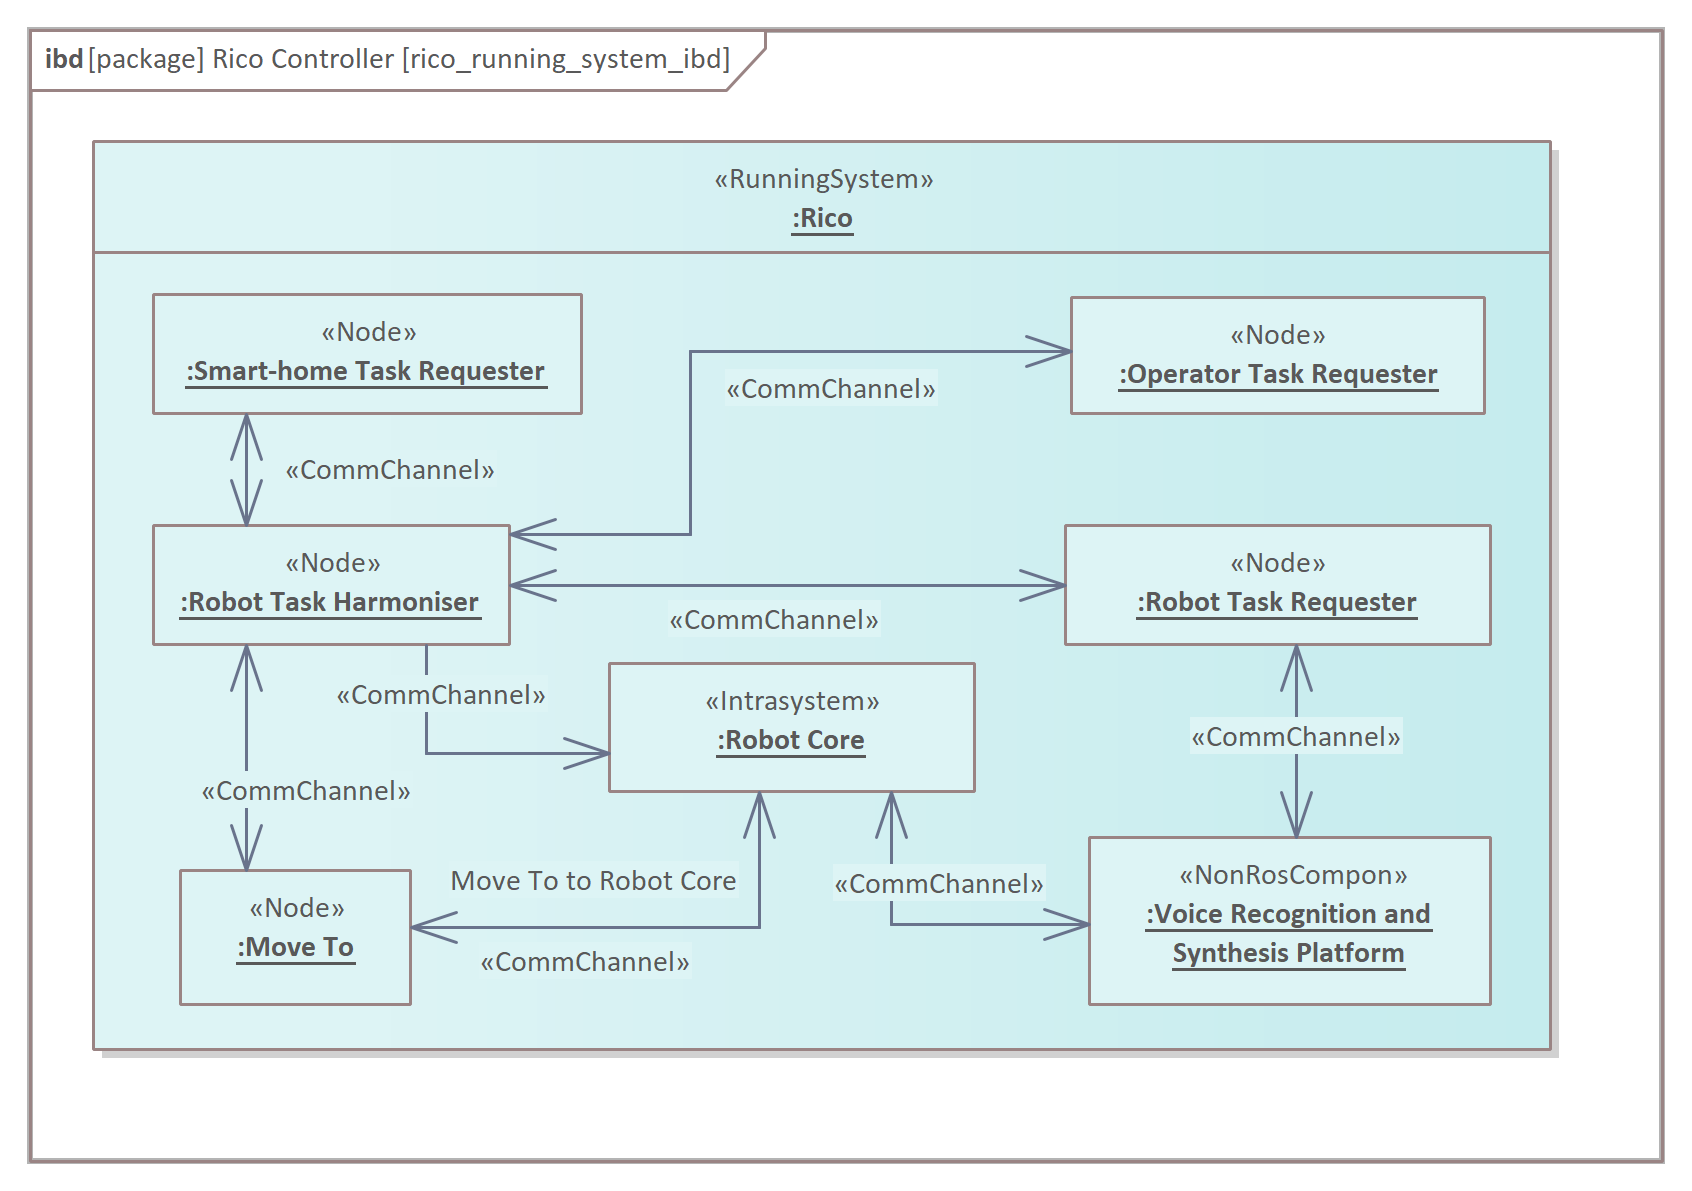
\includegraphics[scale=0.85]{img/rico_pkg/rico_running_system_ibd.png}}
		\end{center}
		\caption{Structure of <<RunningSystem>> \texttt{:Rico} -- ibd.} 
		\label{fig:rico_running_system_ibd}
	\end{figure}

	The system is based on TaskER framework \cite{tasker2020} developed from the RAPP approach to construct systems with variable structure \cite{zielinski2017variable}. The role of the TaskER is to schedule a robot’s tasks. It consists of (i) Task Requesters <<Node>>s to submit new tasks, (ii) Task Harmoniser <<Node>> to schedule tasks execution, (iii) dynamic <<Node>>s (here, <<Node>> \texttt{:Move To}) to execute a particular task on the robot hardware and (iv) cloud part, here <<NonRosCompon>> \texttt{:Voice Recognition and Synthesis Platform}. The common part of the controller is located in <<Intrasystem>> \texttt{:Rico}.
	
	Fig.~\ref{fig:robot_core_ibd} illustrates how various instances of the same block are depicted in the model. Two <<Parameter>> Objects of the same classifier \texttt{:Double} are composed into <<Node>> \texttt{:MoveBase}.
	
	\begin{figure}[H]
		\centering
		\begin{center}
			{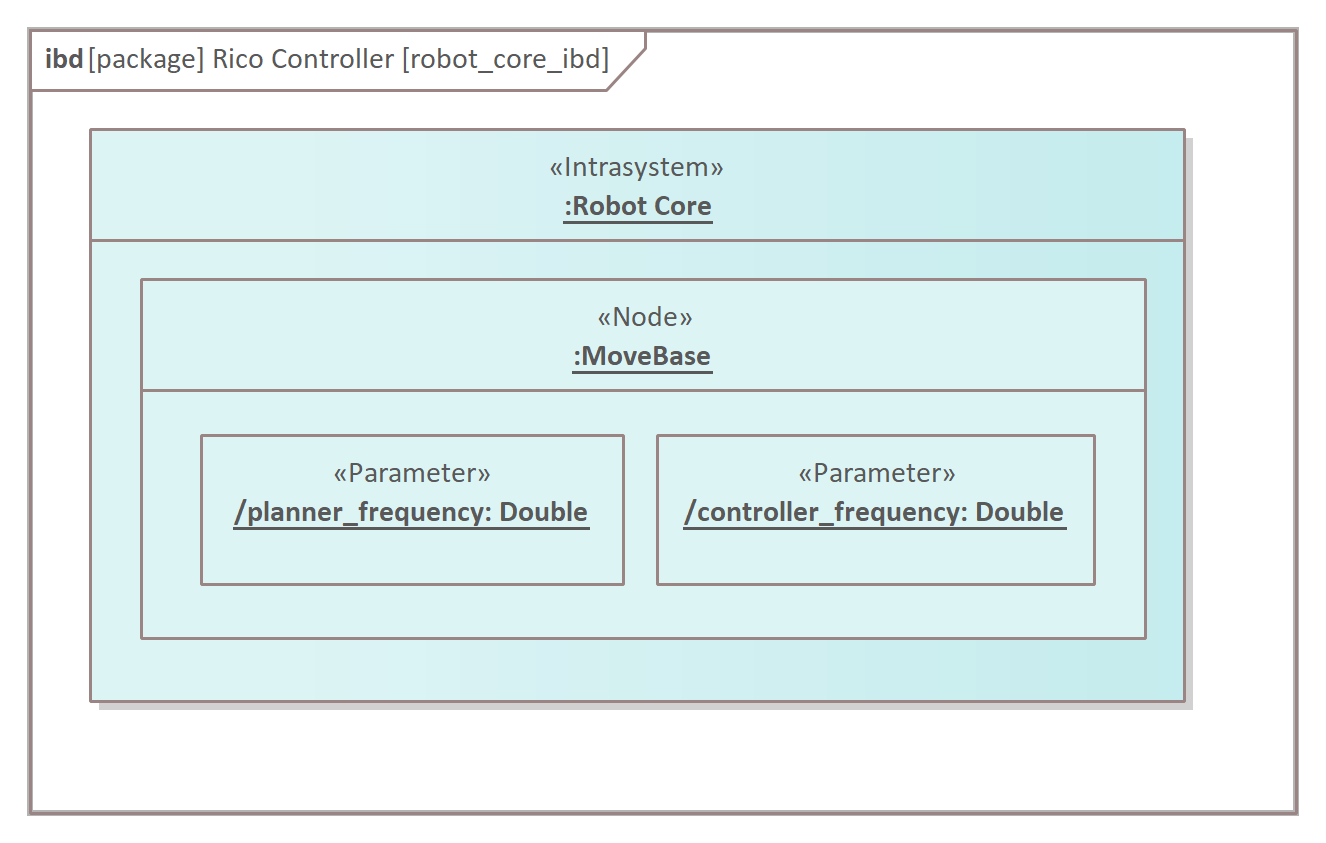
\includegraphics[scale=0.85]{img/rico_pkg/robot_core_ibd.png}}
		\end{center}
		\caption{Selected elements of <<Intrasystem>> \texttt{:Robot Core} -- ibd.} 
		\label{fig:robot_core_ibd}
	\end{figure}
	
			
	<<CommChannel>> \texttt{:Move To to Robot Core} is depicted in Fig.~\ref{fig:move_to_2_core_cm_ibd}. It comprises three actions.
	

	\begin{figure}[H]
		\centering
		\begin{center}
			{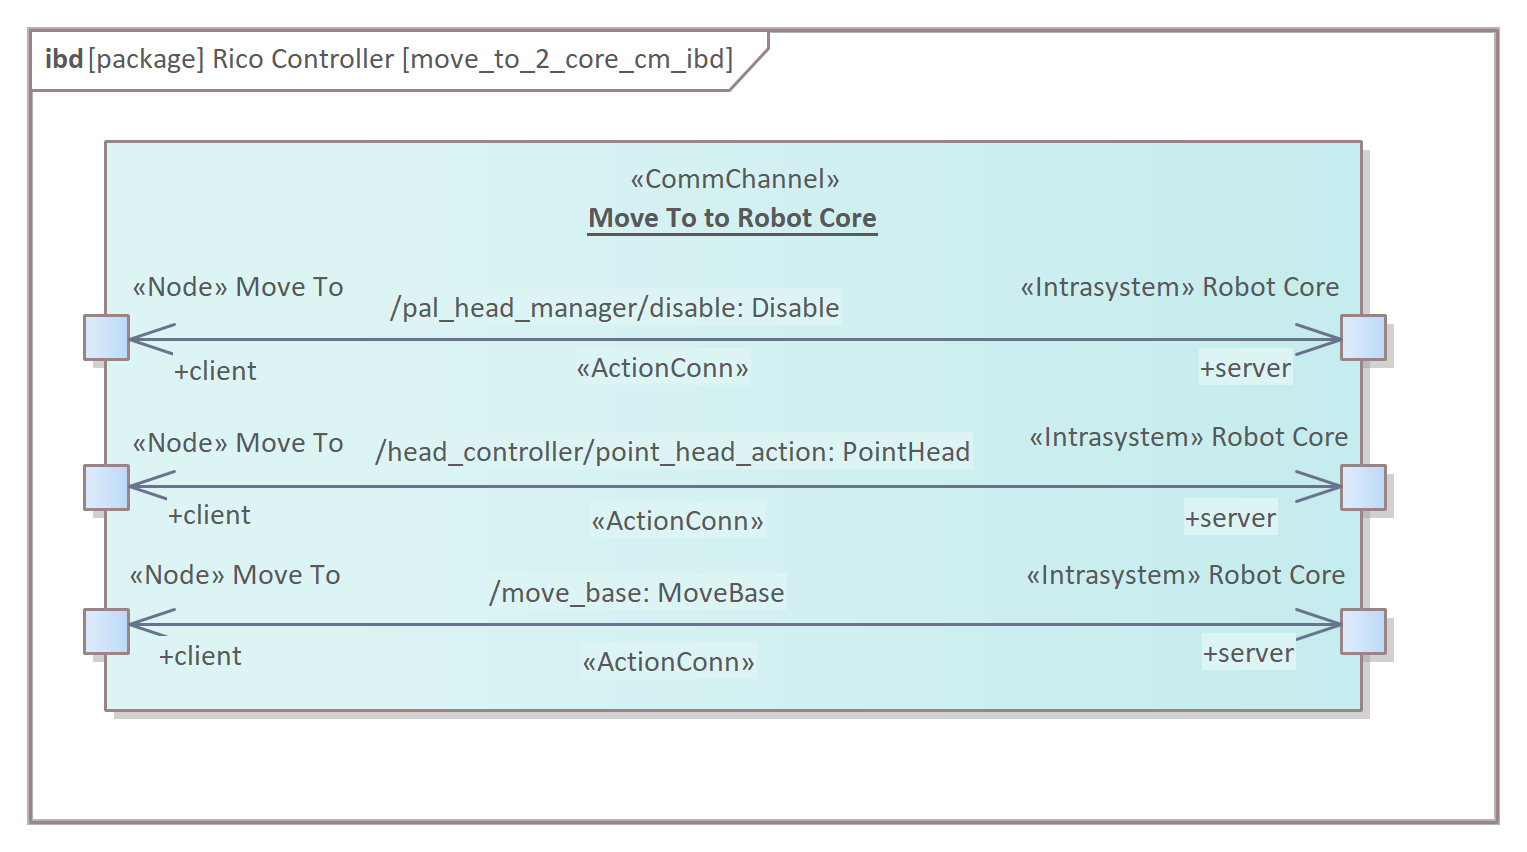
\includegraphics[scale=1.0]{img/rico_pkg/move_to_2_core_cm_ibd.png}}
		\end{center}
		\caption{Example of <<CommChannel>> -- ibd.} 
		\label{fig:move_to_2_core_cm_ibd}
	\end{figure}
	
		
	The part of the scenario generally described in Fig.~\ref{fig:general_sd} is depicted in detail in Fig.~\ref{fig:motion_execution_sd}. The presentation remains conceptual from the behavioural point of view, but it considers the particular parts of the <<RunningSystem>> \texttt{:Rico}.
	
	\begin{figure}[H]
		\centering
		\begin{center}
			{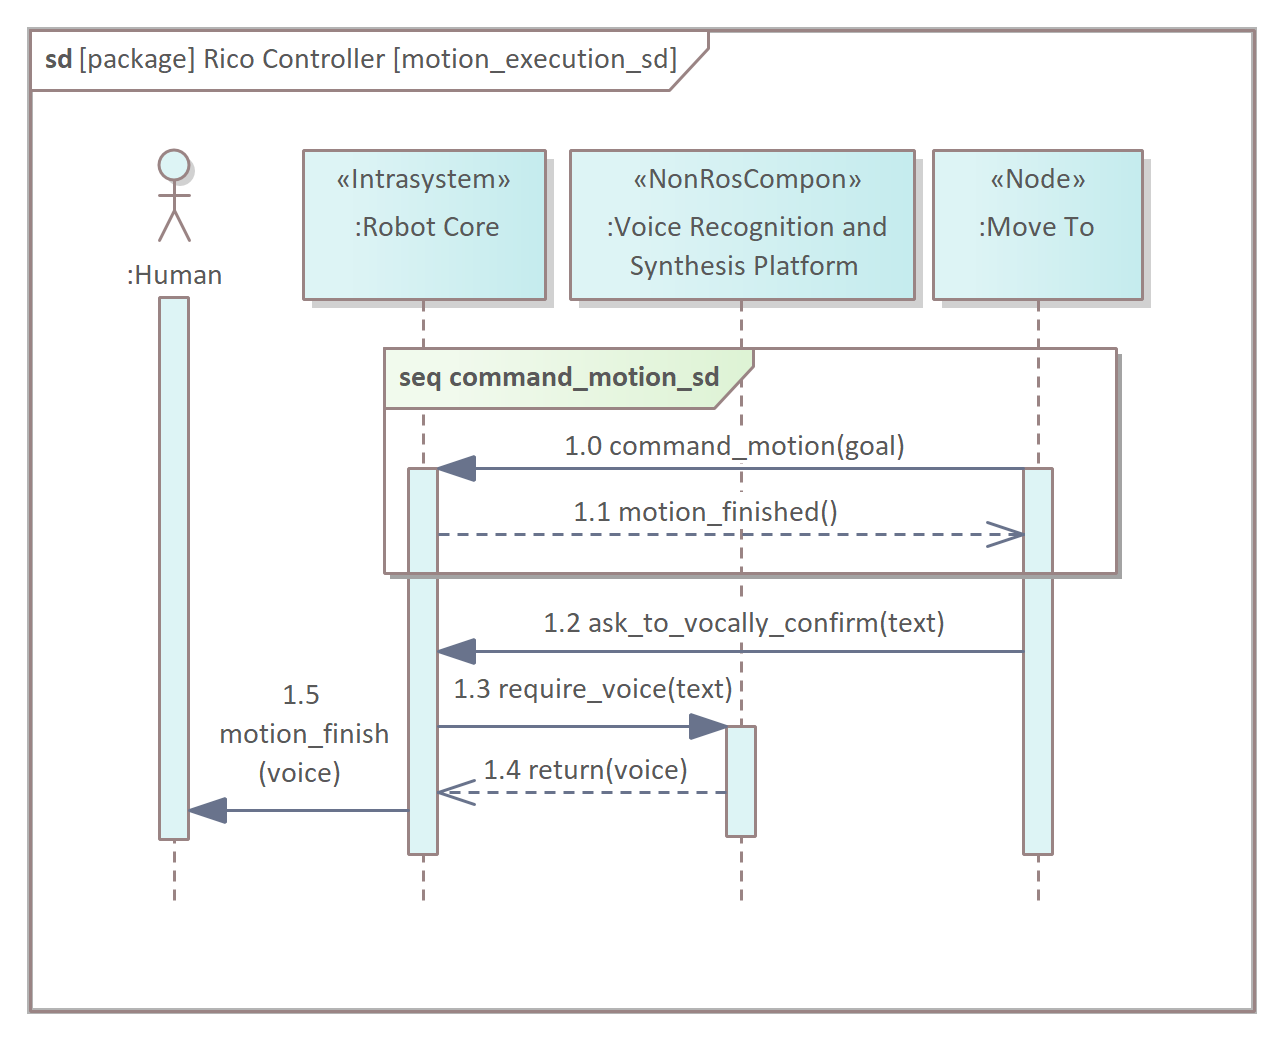
\includegraphics[scale=1.1]{img/rico_pkg/motion_execution_sd.png}}
		\end{center}
		\caption{Motion execution operation -- sd.} 
		\label{fig:motion_execution_sd}
	\end{figure}

\pagebreak


	Finally, the particular communication methods are specified on the most detailed, ROS-specific level (Fig.~\ref{fig:command_motion_sd}). The command\_motion operation includes the sequence of four steps of communication. Three Actions realise the communication, one utilised twice. The diagram comprises extra notes that make it easier to interpret.
	
	\begin{figure}[H]
		\centering
		\begin{center}
			{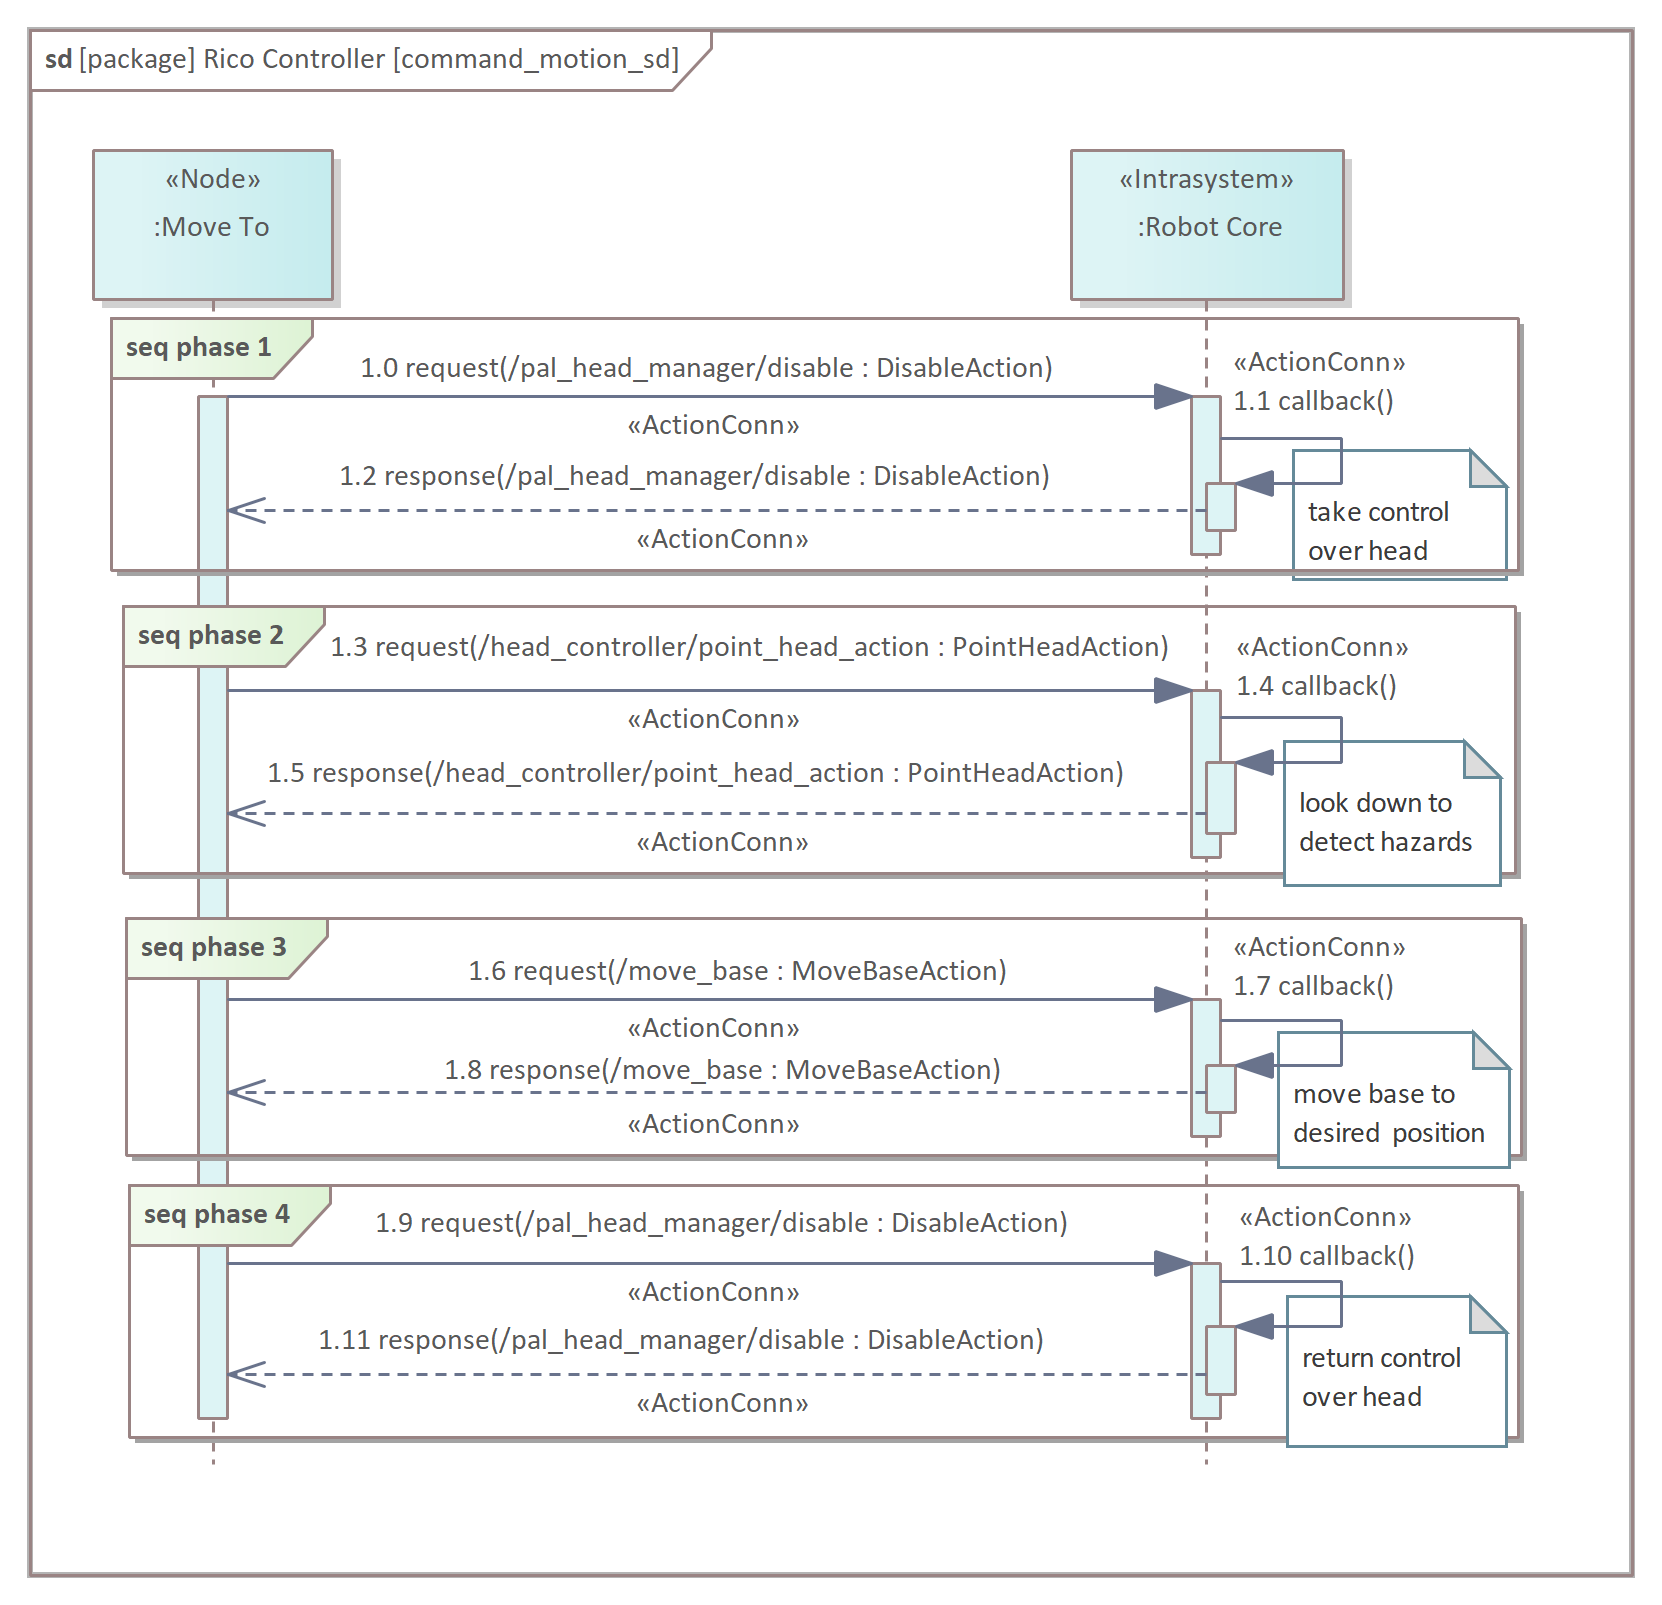
\includegraphics[scale=1.1]{img/rico_pkg/command_motion_sd.png}}
		\end{center}
		\caption{Command motion operation with detailed Communication methods presentation -- sd.} 
		\label{fig:command_motion_sd}
	\end{figure}
	
	\pagebreak
	
	The part of the <<Workspace>> \texttt{:Rico} that includes previously mentioned elements is presented in Fig.~\ref{fig:rico_workspace_nodes_bdd} and Fig.~\ref{fig:rico_workspace_msgs_bdd}.
	
	\begin{figure}[H]
		\centering
		\begin{center}
			{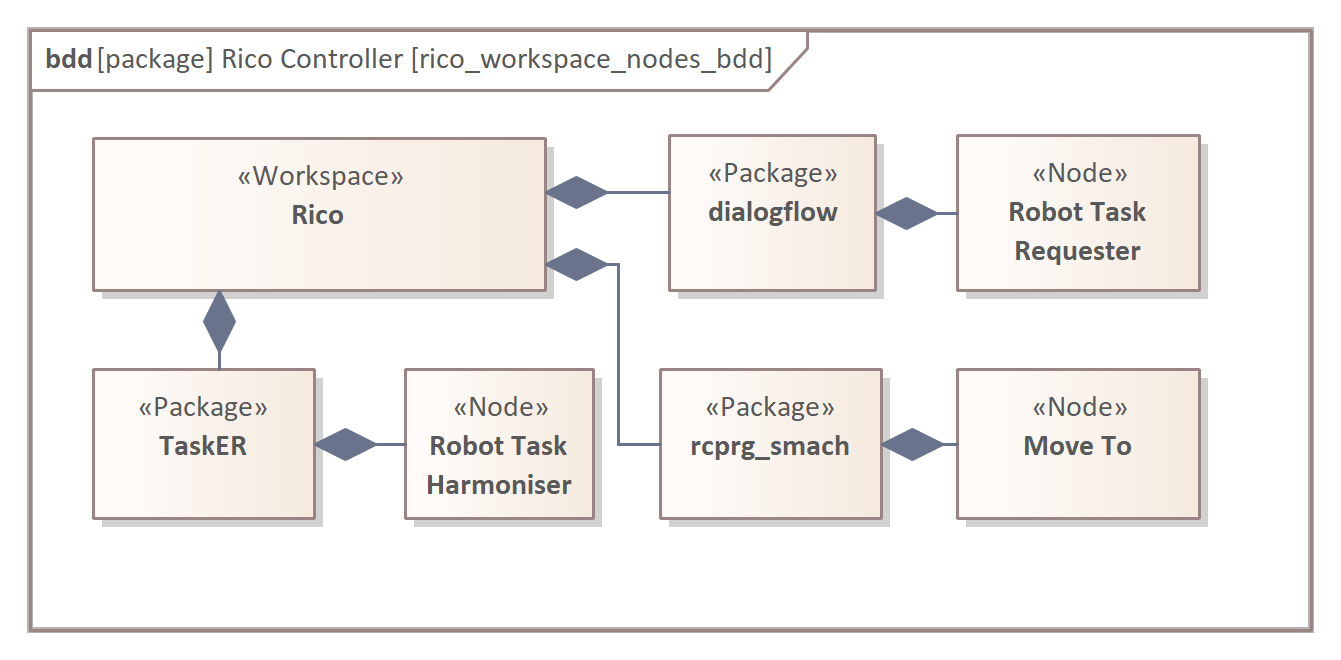
\includegraphics[scale=1.0]{img/rico_pkg/rico_workspace_nodes_bdd.png}}
		\end{center}
		\caption{Rico <<Workspace>> composition -- Packages with Nodes -- bdd.}
		\label{fig:rico_workspace_nodes_bdd}
	\end{figure}

	\begin{figure}[H]
		\centering
		\begin{center}
			{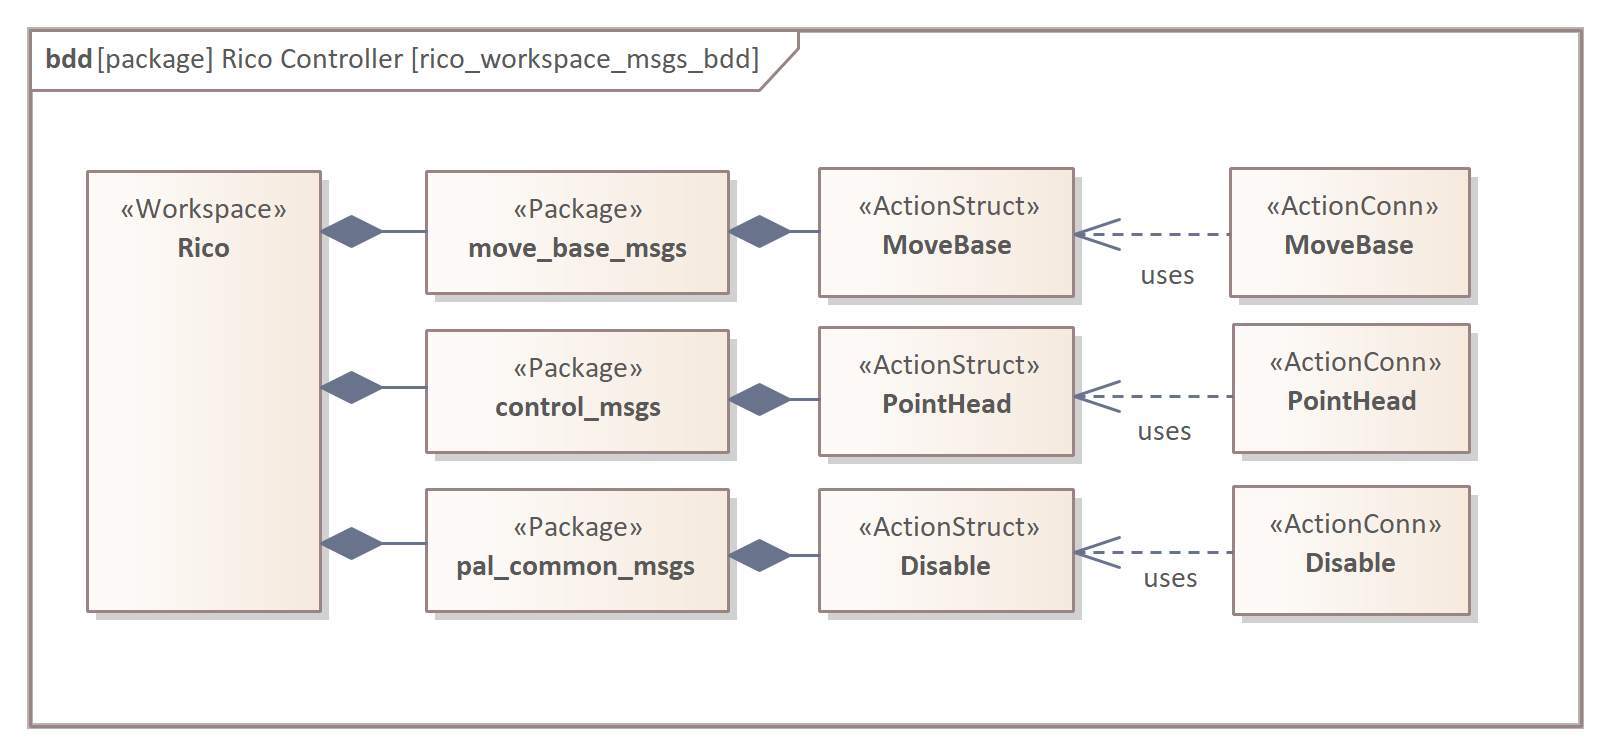
\includegraphics[scale=1.0]{img/rico_pkg/rico_workspace_msgs_bdd.png}}
		\end{center}
		\caption{Rico <<Workspace>> composition -- Packages with Msgs -- bdd.}
		\label{fig:rico_workspace_msgs_bdd}
	\end{figure}
	
			
\AtNextBibliography{\small}
\printbibliography
	
\end{document}
